\chapter{Evaluation and Analysis Results}
The evaluation and analysis result chapter will provide all gathered and analyzed data from the four different test carried out in this thesis. The chapter is divided into different subsections for each test case. 

\section{General Procedure}
Each event have been evaluated and analyzed with the same general procedure. Figure \ref{fig:GeneralProcedure} shows an overview of the steps each event has been through. The results from each event are presented and explained in each sub-section and in some cases, the general procedure has given insights to further analysis which is also covered in the sub-section. The steps of the general procedure are explained throughout this sub-section.

\begin{figure}[H]
    \centering
    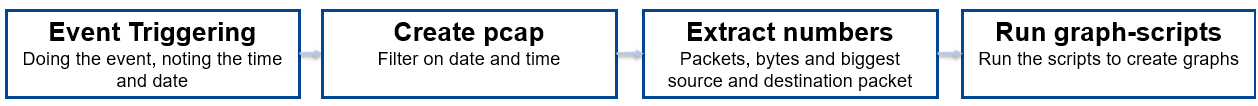
\includegraphics[width=\textwidth]{figures/GeneralProcedure.png}
    \caption{General procedure for evaluation and analysis of test cases}
    \label{fig:GeneralProcedure}
\end{figure}

To be able to run analysis on the data gathered from the different packet capturings (pcaps) and present it in an understandable way, two different programs were used; Wireshark and Visual Studio Code (VS Code) with pyshark, a tshark library. Wireshark were used to extract numbers and calculations from the pcaps and VS Code was used to generate graphs from the pcaps for the events. Even tough it is possible to use Wireshark to generate the same graphs as with VS Code, VS Code was selected because it was easier to generate graphs that have the same measures to compare and they were more ascetically pleasing to look at.
\\\\
When opening a pcap in Wireshark several statistics are possible to extract. By choosing the option of "Capture File Properties", total number of packets and bytes in the capture file are shown and were extracted. The numbers from each pcap were noted down and used as a value to compare both the events to each other and to the baseline. 
\\\\
In VS Code, python was used as the programming language as it includes the library pyshark which can be used towards the tshark capture files. Two scripts with a number of different if statements were used to generate the graphs depending on the users arguments passed to the script. The scripts only differs with if the user wants to display the graphs with number of packets or number of graphs as the measure on the y-axis. The code is displayed in its whole in \ref{app:GraphsByBytes}, \ref{app:GraphsByPackets}, \ref{app:GraphsByBytes_BaselineEvents} and \ref{app:GraphsByPackets_BaselineEvents}, and in pseudo code beneath in algorithm \ref{alg:GraphScript}. For each of the if statements, the same code block is included and are only shown once in algorithm \ref{alg:GraphScript}. The graphs are all generated with bytes and packets per 2 seconds, where the y-axis is defined in the amount of packets or bytes and the x-axis defined as time. The scripts used have have used parts from the scripts explained in \cite{GraphsInspiration}.

Table \ref{tab:SystemArgumentsScripts} displays the different system arguments to be passed to the scripts to create the graphs and which values the arguments expect. 

\begin{table}[H]
    \centering
    \caption{Overview of system arguments for scripts}
    \begin{adjustbox}{width=1\textwidth}
    \begin{tabular}{l|l|l|}
        \cline{2-3} & \textbf{Description} & \textbf{Values}\\ \hline
        \multicolumn{1}{|l|}{\textbf{Argument 1}} & Name of device & \begin{tabular}[c]{@{}l@{}}Netatmo\\ Mill\\ Nedis\end{tabular} \\ \hline
        \multicolumn{1}{|l|}{\textbf{Argument 2}} & Which packets to include & \begin{tabular}[c]{@{}l@{}}Inbound packets and bytes\\ Outbound packets and bytes\\ Inbound and outbound packets and bytes\end{tabular} \\ \hline
        \multicolumn{1}{|l|}{\textbf{Argument 3}} & Type of event & \begin{tabular}[c]{@{}l@{}}Cooking\\ Shower\\ Window\\ Weekend\\ Baseline\end{tabular} \\ \hline
        \multicolumn{1}{|l|}{\textbf{Argument 4}} & Maximum value for y-axis, in bytes or packets & <Numeric value> \\ \hline
    \end{tabular}
    \end{adjustbox}
    \label{tab:SystemArgumentsScripts}
\end{table}

\begin{algorithm}[H]
\caption{Script for generating graphs}\label{alg:GraphScript}
    \begin{algorithmic}[1]
        \For{Each date of event} \Comment{Graph\_function start}
            \State Extract the packets from the right pcap
            \For{Each packet in pcap}
                \State Extract packet length in byte and time or add packet count to time
                \State Display graph
            \EndFor
        \EndFor \Comment{Graph\_function end}\\
        \If{Argument 2 is Outbound} \Comment{Set display filter to outbound traffic}
            \If{Argument 1 is Netatmo}
                \State Set display filter to "wlan.sa == Netatmo MAC address"
            \ElsIf{Argument 1 is Mill}
                \State Set display filter to "wlan.sa == Mill MAC address"
            \ElsIf{Argument 1 is Nedis}
                \State Set display filter to "wlan.sa == Nedis MAC address"    
            \EndIf \\
        \ElsIf{Argument 2 is Inbound} \Comment{Set display filter to inbound traffic}
            \If{Argument 1 is Netatmo}
                \State Set display filter to "wlan.da == Netatmo MAC address"
            \ElsIf{Argument 1 is Mill}
                \State Set display filter to "wlan.da == Mill MAC address"
            \ElsIf{Argument 1 is Nedis}
                \State Set display filter to "wlan.da == Nedis MAC address"  
            \EndIf
        \EndIf \\
        \If{Argument 3 is Shower} \Comment{Event if-cases start}
            \State Set the dates from when the events occurred 
            \State Graph\_function
        \ElsIf{Argument 3 is Cooking}
            \State Set the dates from when the events occurred 
            \State Graph\_function
        \ElsIf{Argument 3 is Window}
            \State Set the dates from when the events occurred 
            \State Graph\_function
        \ElsIf{Argument 3 is Weekend}
            \State Set the dates from when the events occurred 
            \State Graph\_function
        \ElsIf{Argument 3 is Baseline}
            \State Set the dates from when the events occurred 
            \State Graph\_function
        \EndIf \Comment{Event if-cases end}
    \end{algorithmic}
\end{algorithm}

To create a file for each of the events, a time filter was applied to the pcaps and then the remaining packets exported to a separate pcap which can be opened in Wireshark or make a graph out of to analyze each specific event. The time filter used followed the following format:

\begin{itemize}
\item \textbf{Format:} frame.time >= "Month Date, Year "Time"" \&\& frame.time <= "Month Date, Year "Time""//
\item \textbf{Example:} frame.time >= "Jan 08, 2023 "19:30:00"" \&\& frame.time <= "Jan 08, 2023 "20:40:00""
\end{itemize}

\section{Baseline}
The capturing of baseline traffic were conducted over the course of 10 days in the same environment as the devices were when conducting the events. During the baseline, the devices have not been affected by the specific events, such as cooking, showering or window open in the same room as the devices resides. The baseline traffic will be used to look at standard traffic from the devices and to compare this to the events in both graphs and calculations in Sub-section 5.3-5.5. The traffic from the capture files were encrypted on layer 2 (Wi-Fi) and therefore it is not possible to extract any values from the payload of the packets. This applies to all the devices. Since looking into decryption of the traffic is out of scope for this thesis, the results will only analyze patterns and no payload information. 
\\\\
The filter used for all the baseline files are:

\begin{itemize}
\item frame.time >= "Mar 06, 2023 "00:00:00"" \&\& frame.time <= "Mar 15, 2023 "24:00:00""
\end{itemize}

\subsection{Netatmo Baseline}
Figure \ref{fig:NetatmoBaselineTotalPackets} and \ref{fig:NetatmoBaselineTotalBytes} shows the graphs for Netatmo from the baseline capturing from 6th of March 2023 to 15th of March 2023. 
\begin{figure} [H]
    \centering
    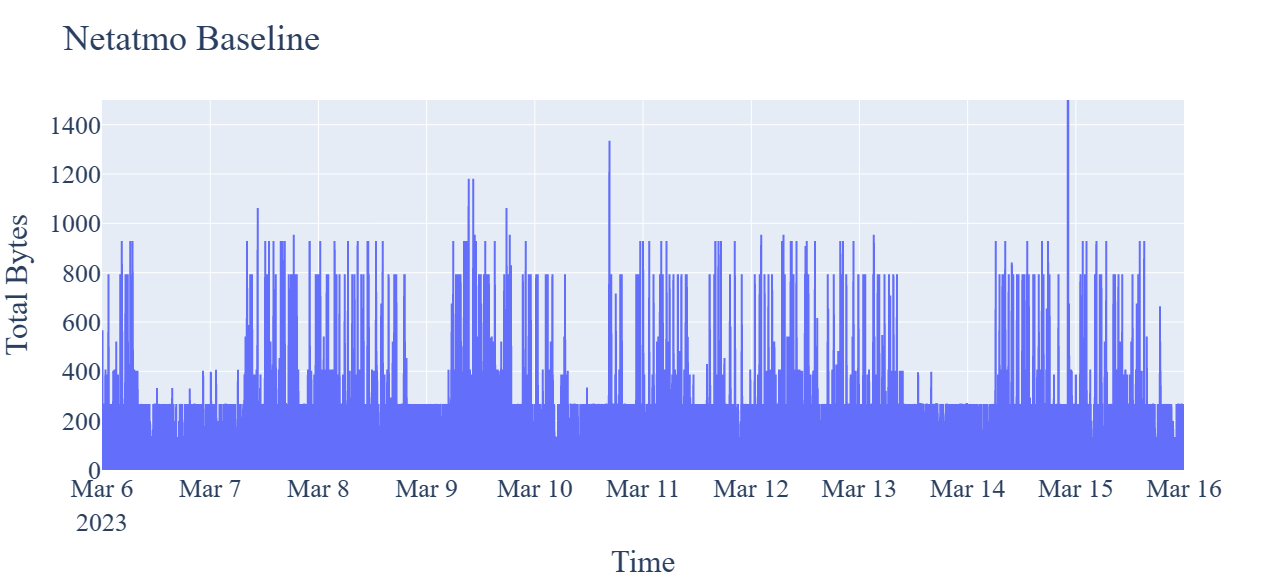
\includegraphics[scale=0.3]{figures/Netatmo_Baseline_TotalBytes.png}
    \caption{Netatmo baseline capture with total number of bytes as the y-axis}
    \label{fig:NetatmoBaselineTotalBytes}
\end{figure}

\begin{figure} [H]         
    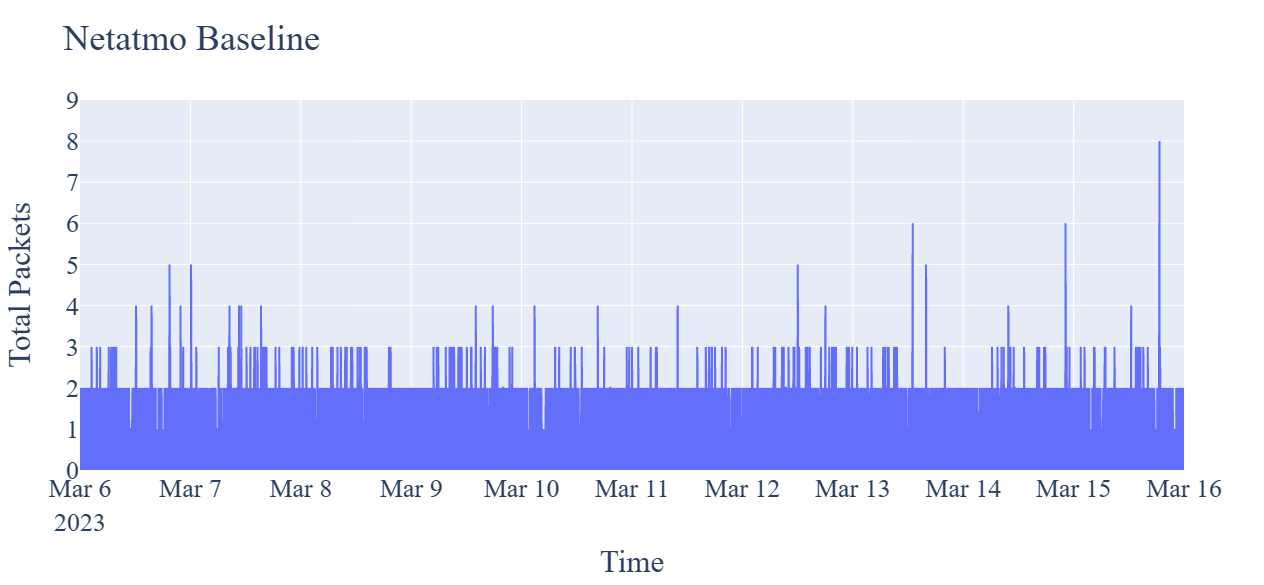
\includegraphics[scale=0.3]{figures/Netatmo_Baseline_TotalPackets.png}
    \caption{Netatmo baseline capture with total number of packets as the y-axis}
    \label{fig:NetatmoBaselineTotalPackets}
 \end{figure}

For the baseline graphs, it is possible to see that packets are sent continually at a rate of around 250 bytes per 2 seconds and 2 packets per 2 seconds. In addition to the continuously stream of packets, the traffic flow also has spikes that looks random in both time and size. As these graphs shows the total packets and bytes sent and received, it can also be beneficial to look at what the graphs would look like if filtered on packets and bytes sent and packets and bytes received separately. 

 \begin{figure}[H]
    \centering
    \begin{subfigure}[b]{0.4\textwidth}
        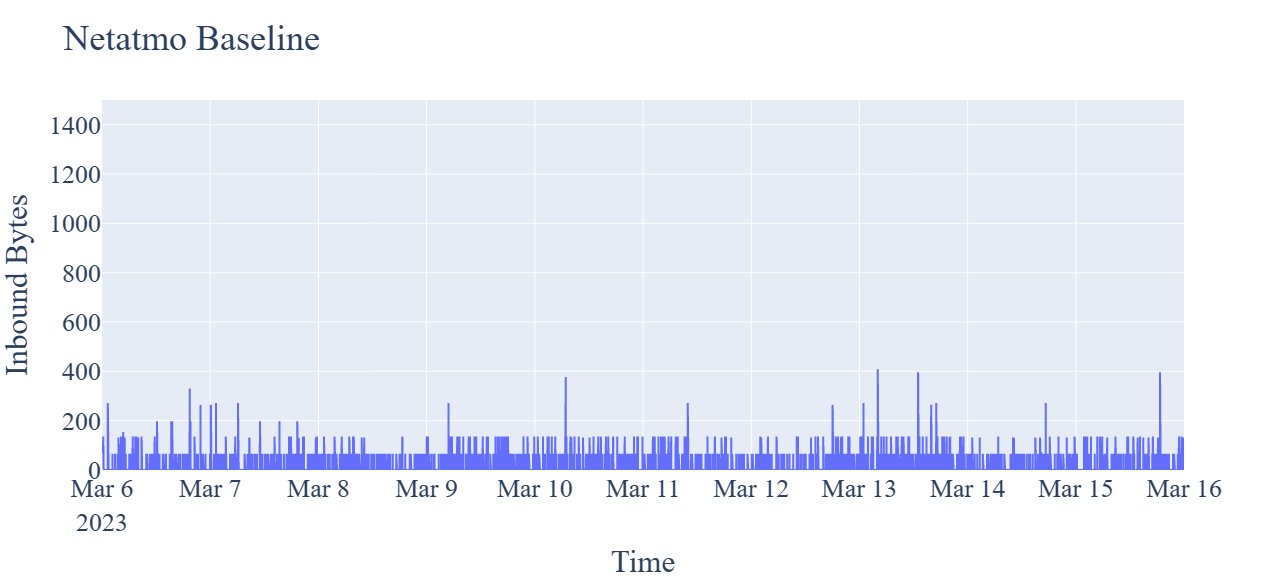
\includegraphics[width=\textwidth]{figures/Netatmo_Baseline_InboundBytes.png}
        \caption{Netatmo inbound bytes}
    \end{subfigure}
    \begin{subfigure}[b]{0.4\textwidth}
        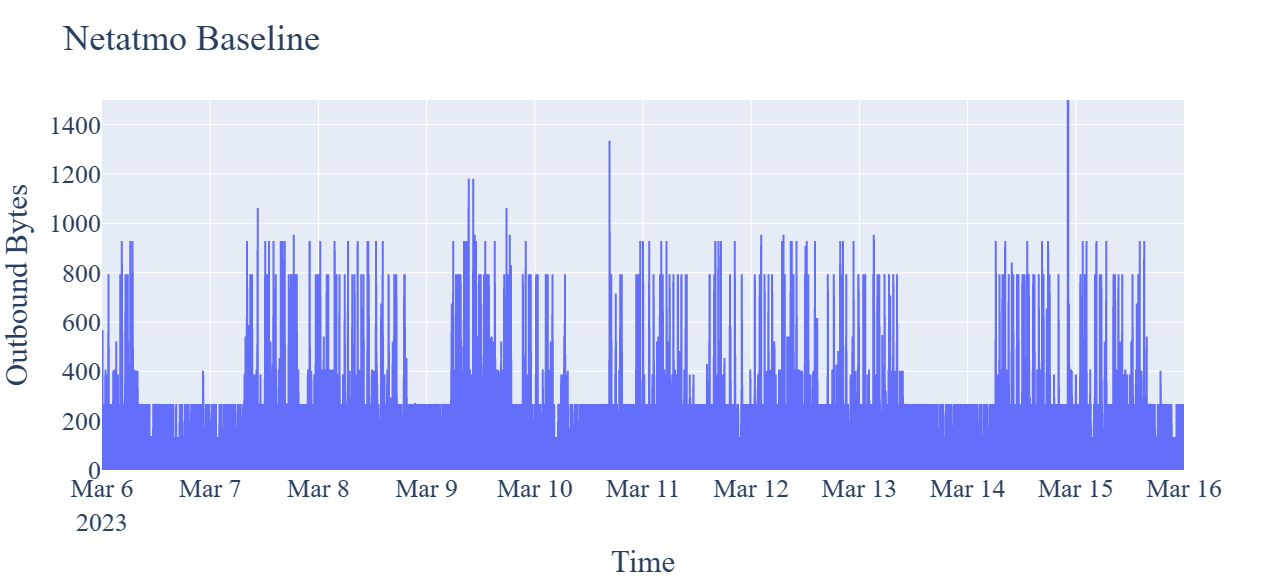
\includegraphics[width=\textwidth]{figures/Netatmo_Baseline_OutboundBytes.png}
        \caption{Netatmo outbound bytes}
    \end{subfigure}
    \begin{subfigure}[b]{0.4\textwidth}
        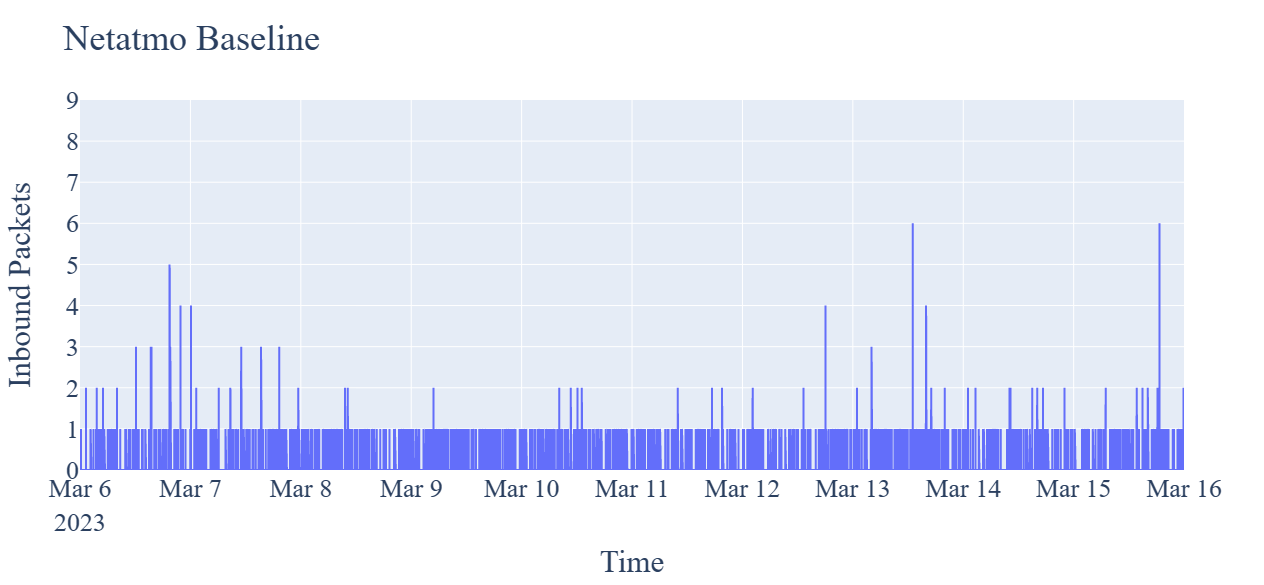
\includegraphics[width=\textwidth]{figures/Netatmo_Baseline_InboundPackets.png}
        \caption{Netatmo inbound packets}
    \end{subfigure}
    \begin{subfigure}[b]{0.4\textwidth}
        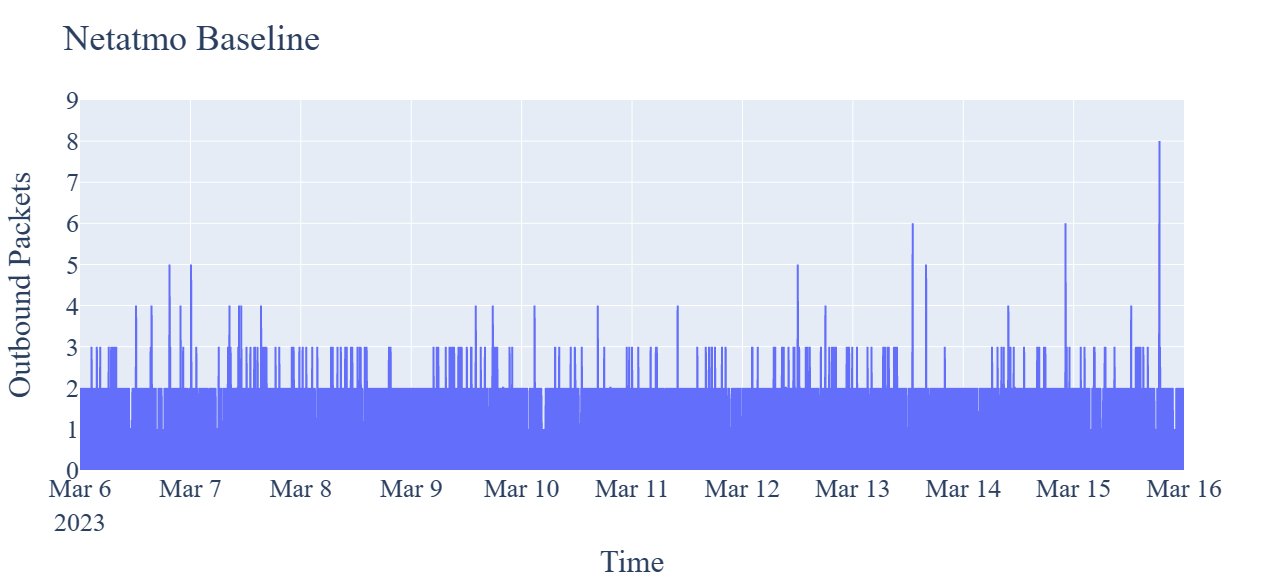
\includegraphics[width=\textwidth]{figures/Netatmo_Baseline_OutboundPackets.png}
        \caption{Mill outbound packets}
    \end{subfigure}
    \caption{Netatmo baseline inbound and outbound bytes}
    \label{Fig:NetatmoBaselineOutandInboundTraffic}
 \end{figure}

For the inbound and outbound bytes and packets for Netatmo, Figure \ref{Fig:NetatmoBaselineOutandInboundTraffic}, it is clear to see that the device sends a lot more than it receives. Calculations made on the baseline traffic are presented in Table \ref{tab:NetatmoBaselineCalculations}. 

\begin{table}[H]
    \caption{Calculations for Netatmo baseline capture}
    \centering
    \begin{tabular}{ll|l|}
        \cline{3-3}                                               &                               &             \textbf{Numbers} \\ \hline
        \multicolumn{1}{|c|}{\multirow{4}{*}{\textbf{Total}}}    & Packets              & 110,735         \\ \cline{2-3} 
        \multicolumn{1}{|c|}{}                                   & Bytes                & 14,959,396       \\ \cline{2-3} 
        \multicolumn{1}{|c|}{}                                   & Average bytes/second & 17               \\ \cline{2-3} 
        \multicolumn{1}{|c|}{}                                   & Average packet size  & 135 bytes        \\ \hline
        \multicolumn{1}{|l|}{\multirow{5}{*}{\textbf{Inbound}}}  & Packets              & 1,042            \\ \cline{2-3} 
        \multicolumn{1}{|l|}{}                                   & Bytes                & 83,446           \\ \cline{2-3} 
        \multicolumn{1}{|l|}{}                                   & Average bytes/second & 0                \\ \cline{2-3} 
        \multicolumn{1}{|l|}{}                                   & Average packet size  & 80 bytes          \\ \cline{2-3} 
        \multicolumn{1}{|l|}{}                                   & Biggest packet       & 377 bytes        \\ \hline
        \multicolumn{1}{|l|}{\multirow{5}{*}{\textbf{Outbound}}} & Packets              & 109,693          \\ \cline{2-3} 
        \multicolumn{1}{|l|}{}                                   & Bytes                & 14,875,950       \\ \cline{2-3} 
        \multicolumn{1}{|l|}{}                                   & Average bytes/second & 17               \\ \cline{2-3} 
        \multicolumn{1}{|l|}{}                                   & Average packet size  & 136 bytes         \\ \cline{2-3} 
        \multicolumn{1}{|l|}{}                                   & Biggest packet       & 1,150 bytes       \\ \hline
    \end{tabular}
    \label{tab:NetatmoBaselineCalculations}
\end{table}
Comparing the inbound and outbound graphs in Figure \ref{Fig:NetatmoBaselineOutandInboundTraffic} with the total graphs, in Figure \ref{fig:NetatmoBaselineTotalBytes} and Figure \ref{fig:NetatmoBaselineTotalPackets}, shows that the outbound graphs stands for a majority of the packets and they are very similar to the total graphs. The same is numerically shown in Table \ref{tab:NetatmoBaselineCalculations}, where over 99\% of the total packets are outbound traffic. Therefore, it will be better to only display the events with graphs for total traffic to evaluate and analyze for the rest of the thesis. 

\subsection{Mill Baseline}
Figure \ref{fig:MillBaselineTotalPackets} and \ref{fig:MillBaselineTotalBytes} shows the graphs for Mill from the baseline capturing from 6th of March 2023 to 15th of March 2023. 
\begin{figure} [H]
    \centering
    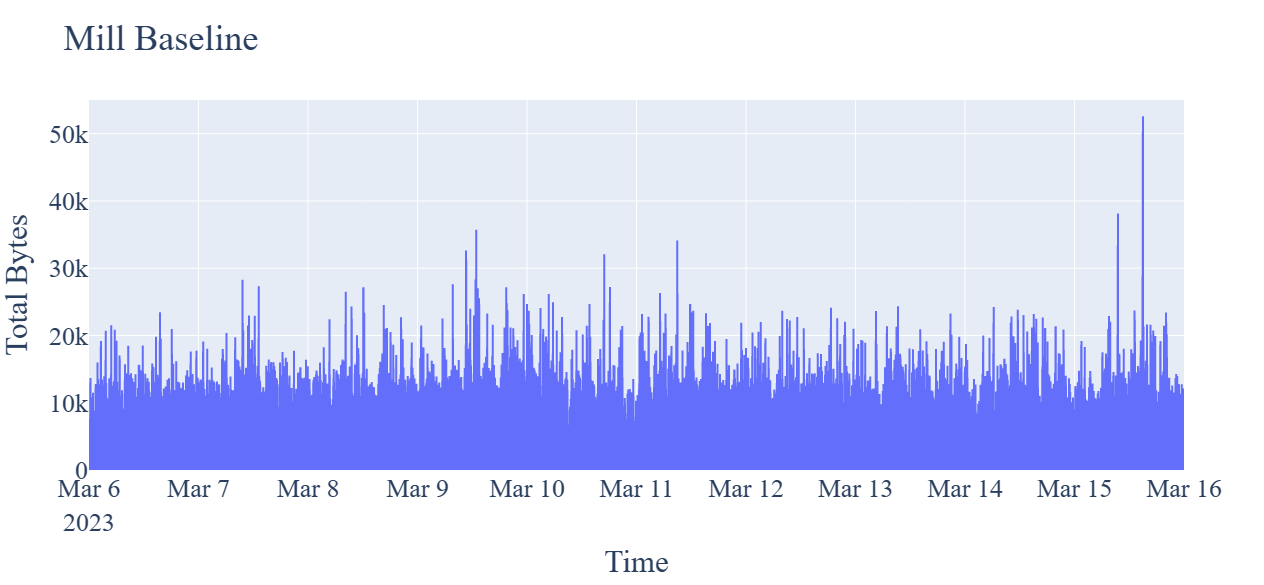
\includegraphics[scale=0.3]{figures/Mill_Baseline_TotalBytes.png}
    \caption{Mill baseline capture with total number of bytes as the y-axis}
    \label{fig:MillBaselineTotalBytes}
\end{figure}

\begin{figure} [H]
    \centering
    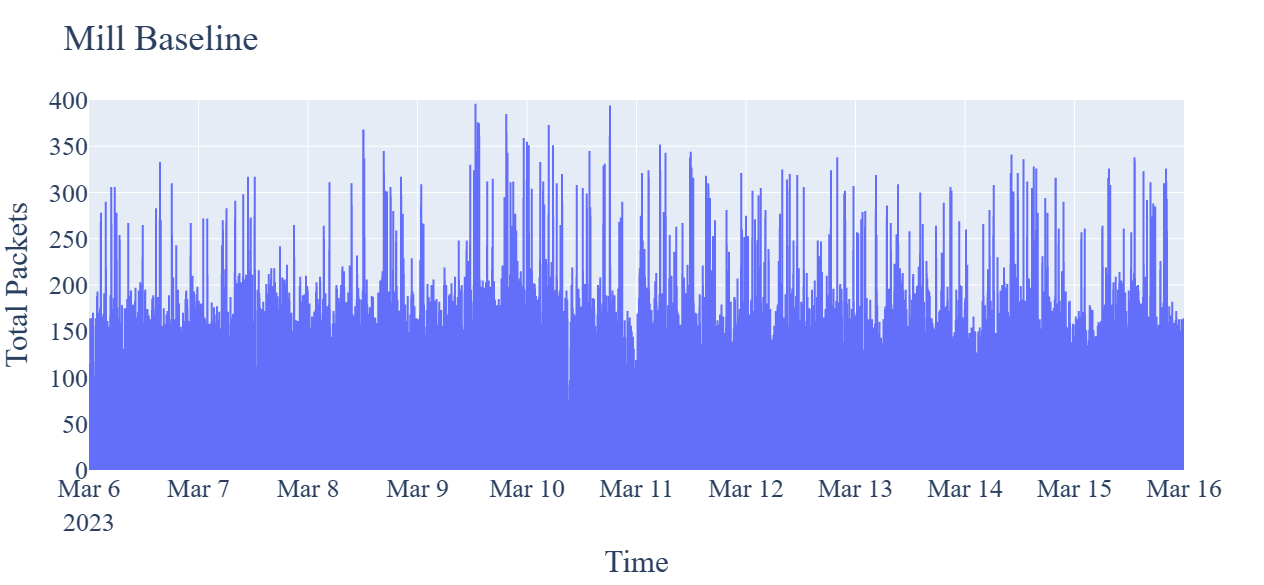
\includegraphics[scale=0.3]{figures/Mill_Baseline_TotalPackets.png}
    \caption{Mill baseline capture with total number of packets as the y-axis}
    \label{fig:MillBaselineTotalPackets}
 \end{figure}

The baseline traffic for Mill shows that the traffic varies a lot. As this device does not send live updates, but every minute, more spikes are included as it does not always send packets. It is also possible to see the spikes more clearly if the time range is smaller, this will be visible further when looking at the event and baseline comparison graphs for each event. 
\\\\
Graphs for inbound and outbound traffic have also been made for Mill to see the differences for the packets sent. Figure \ref{Fig:MillBaselineOutandInboundTraffic} displays the different graphs for each of the traffic directions. Numerical calculations for the baseline traffic are presented in Table \ref{tab:MillBaselineCalculations}. 

\begin{figure}[H]
    \centering
    \begin{subfigure}[b]{0.4\textwidth}
        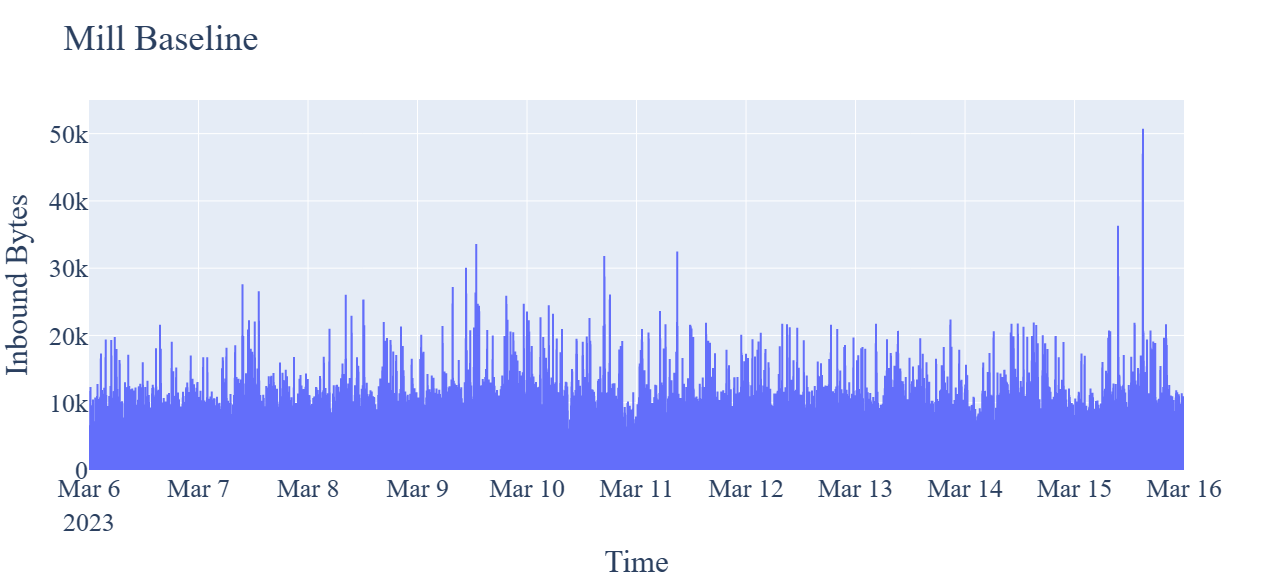
\includegraphics[width=\textwidth]{figures/Mill_Baseline_InboundBytes.png}
        \caption{Mill inbound bytes}
    \end{subfigure}
    \begin{subfigure}[b]{0.4\textwidth}
        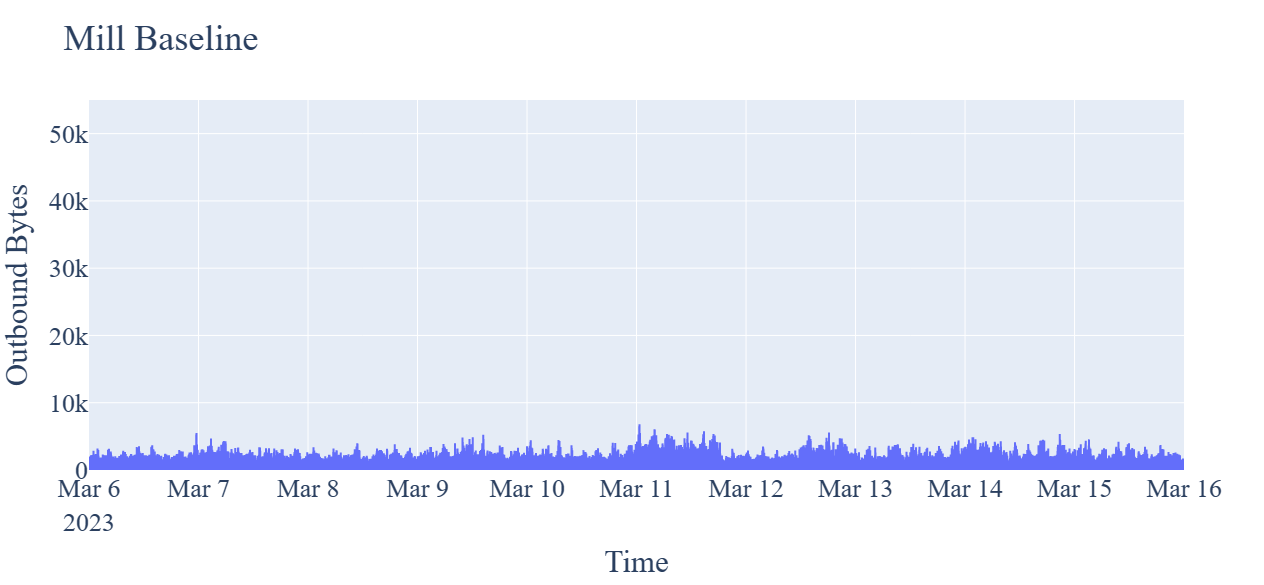
\includegraphics[width=\textwidth]{figures/Mill_Baseline_OutboundBytes.png}
        \caption{Mill outbound bytes}
    \end{subfigure}
    \begin{subfigure}[b]{0.4\textwidth}
        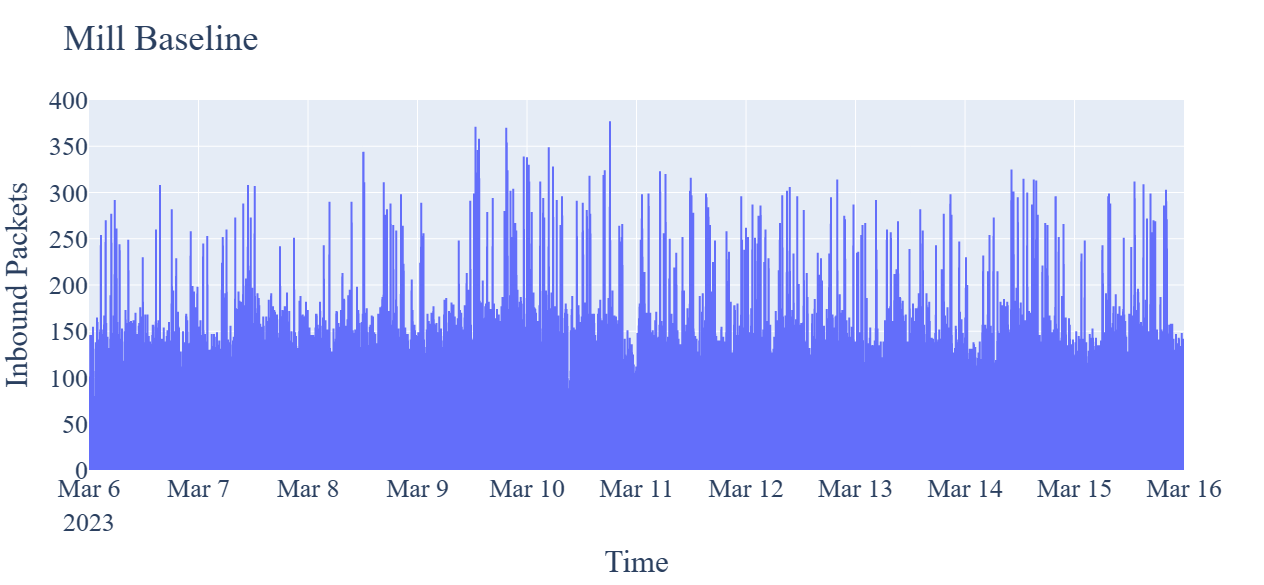
\includegraphics[width=\textwidth]{figures/Mill_Baseline_InboundPackets.png}
        \caption{Mill inbound packets}
    \end{subfigure}
    \begin{subfigure}[b]{0.4\textwidth}
        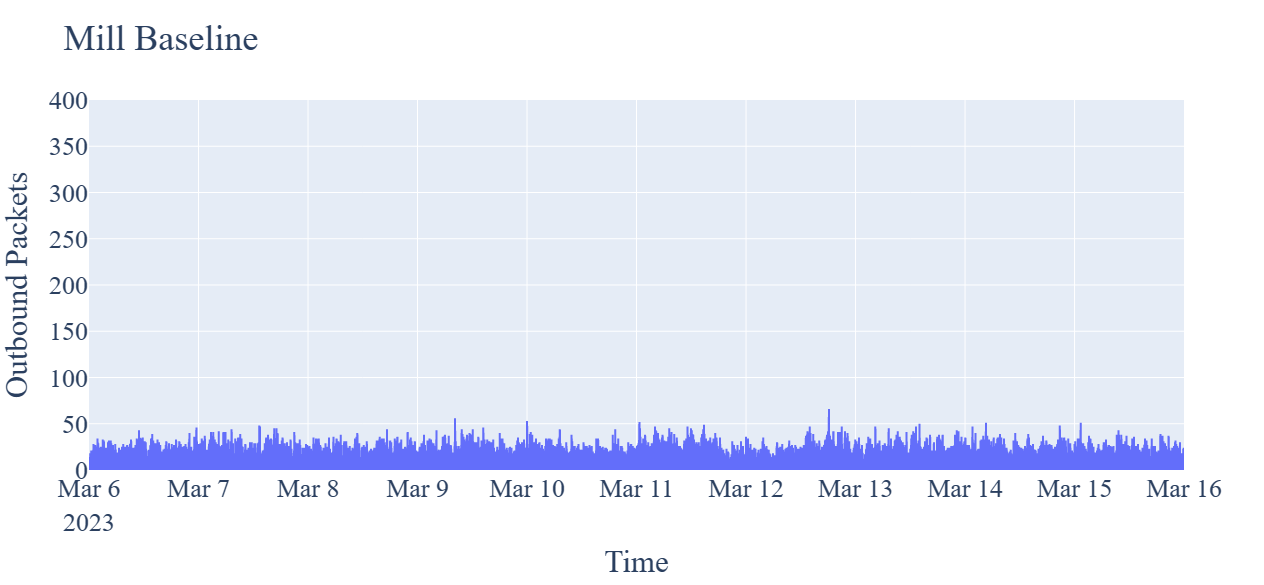
\includegraphics[width=\textwidth]{figures/Mill_Baseline_OutboundPackets.png}
        \caption{Mill outbound packets}
    \end{subfigure}
    \caption{Mill baseline inbound and outbound bytes}
    \label{Fig:MillBaselineOutandInboundTraffic}
 \end{figure}

\begin{table}[H]
    \caption{Calculations for Mill baseline capture}
    \centering
    \begin{tabular}{ll|l|}
        \cline{3-3}                                              &                      & \textbf{Numbers} \\ \hline
        \multicolumn{1}{|c|}{\multirow{4}{*}{\textbf{Total}}}    & Packets              & 1,236,753       \\ \cline{2-3} 
        \multicolumn{1}{|c|}{}                                   & Bytes                & 129,253,290     \\ \cline{2-3} 
        \multicolumn{1}{|c|}{}                                   & Average bytes/second & 149             \\ \cline{2-3} 
        \multicolumn{1}{|c|}{}                                   & Average packet size  & 105 bytes       \\ \hline
        \multicolumn{1}{|l|}{\multirow{5}{*}{\textbf{Inbound}}}  & Packets              & 942,112         \\ \cline{2-3} 
        \multicolumn{1}{|l|}{}                                   & Bytes                & 95,458,773      \\ \cline{2-3} 
        \multicolumn{1}{|l|}{}                                   & Average bytes/second & 110             \\ \cline{2-3} 
        \multicolumn{1}{|l|}{}                                   & Average packet size  & 101 bytes       \\ \cline{2-3} 
        \multicolumn{1}{|l|}{}                                   & Biggest packet       & 1593 bytes      \\ \hline
        \multicolumn{1}{|l|}{\multirow{5}{*}{\textbf{Outbound}}} & Packets              & 294,640         \\ \cline{2-3} 
        \multicolumn{1}{|l|}{}                                   & Bytes                & 33,794,517      \\ \cline{2-3} 
        \multicolumn{1}{|l|}{}                                   & Average bytes/second & 39              \\ \cline{2-3} 
        \multicolumn{1}{|l|}{}                                   & Average packet size  & 115 bytes       \\ \cline{2-3} 
        \multicolumn{1}{|l|}{}                                   & Biggest packet       & 456 bytes       \\ \hline
    \end{tabular}
    \label{tab:MillBaselineCalculations}
\end{table}

As Figure \ref{Fig:MillBaselineOutandInboundTraffic} shows, the device receives a lot more packets and bytes than it sends off. As the inbound graphs do not differ much from the total graphs, it will be best to proceed with the analysis in a total traffic aspect where both inbound and outbound traffic are included. This is also reflected in Table \ref{tab:MillBaselineCalculations}, which shows that 76\% of packets and 74\% of bytes are inbound traffic.

\subsection{Nedis Baseline}
Figure \ref{fig:NedisBaselineTotalPackets} and \ref{fig:NedisBaselineTotalBytes} shows the graphs for Nedis from the baseline capturing from 6th of March 2023 to 15th of March 2023. 
\begin{figure} [H]
    \centering
    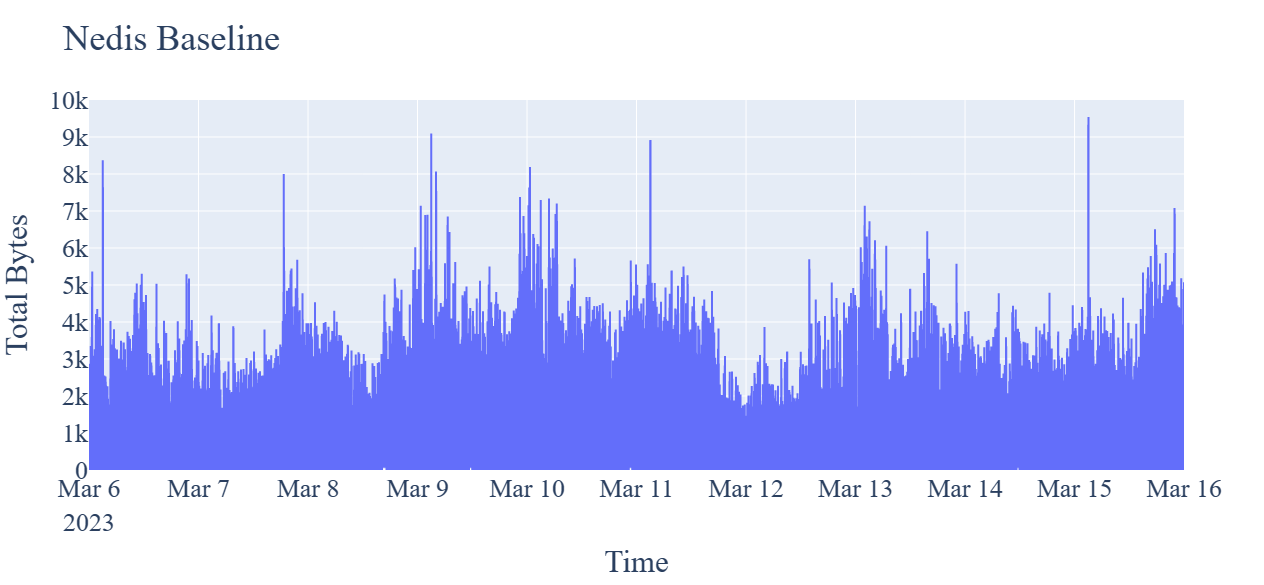
\includegraphics[scale=0.3]{figures/Nedis_Baseline_TotalBytes.png}
    \caption{Nedis baseline capture with total number of bytes as the y-axis}
    \label{fig:NedisBaselineTotalBytes}
\end{figure}

\begin{figure} [H]         
    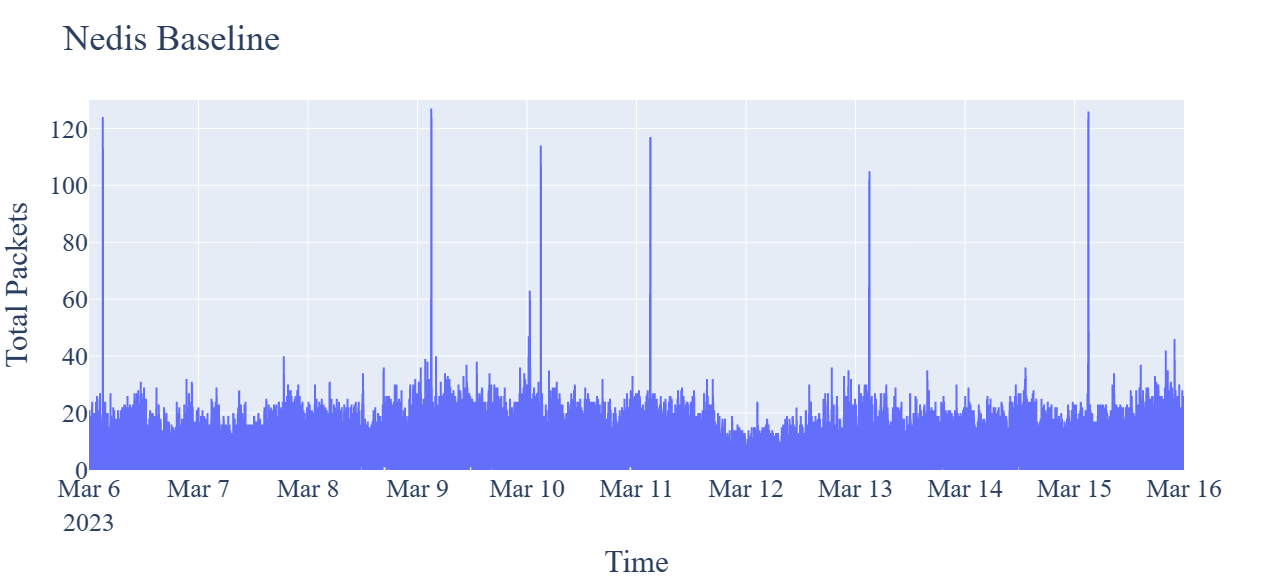
\includegraphics[scale=0.3]{figures/Nedis_Baseline_TotalPackets.png}
    \caption{Nedis baseline capture with total number of packets as the y-axis}
    \label{fig:NedisBaselineTotalPackets}
 \end{figure}

The traffic sent and received by Nedis is characterized by varying a lot with high spikes especially for packets. The larger spikes, which are more visible in Figure \ref{fig:NedisBaselineTotalPackets}, showing the packets, occurs almost everyday. Since traffic is encrypted, it is not possible to see what these spikes are, but for further analysis it is important to understand that normal traffic for the device, can be large spikes occurring around the same time each night around 3am. 

\begin{figure}[H]
    \centering
    \begin{subfigure}[b]{0.4\textwidth}
        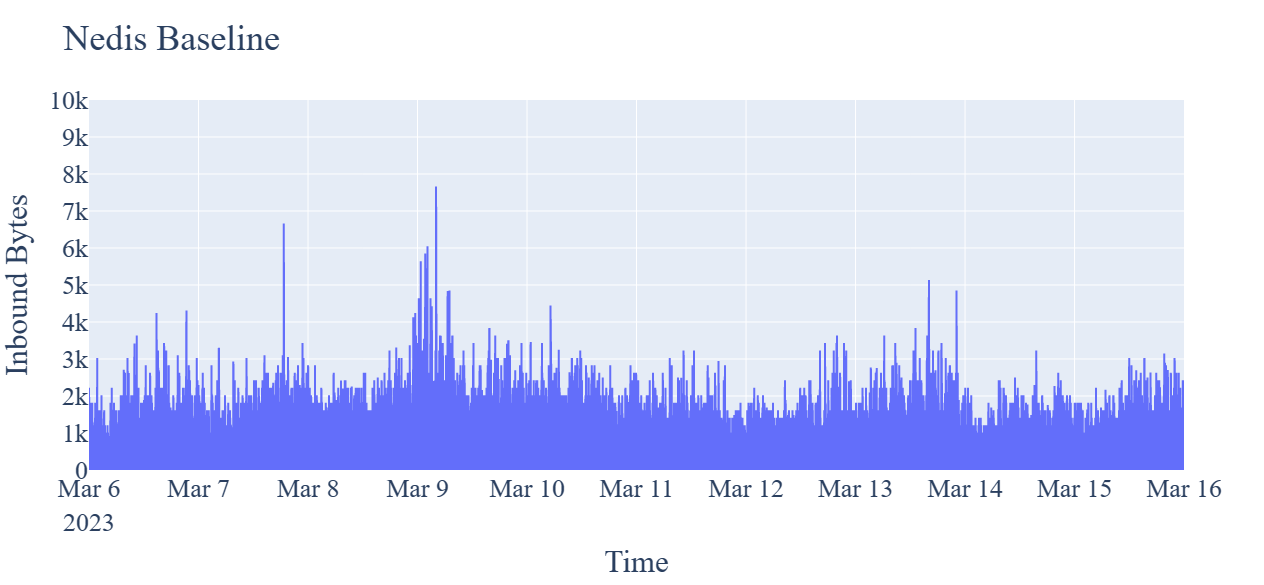
\includegraphics[width=\textwidth]{figures/Nedis_Baseline_InboundBytes.png}
        \caption{Nedis inbound bytes}
    \end{subfigure}
    \begin{subfigure}[b]{0.4\textwidth}
        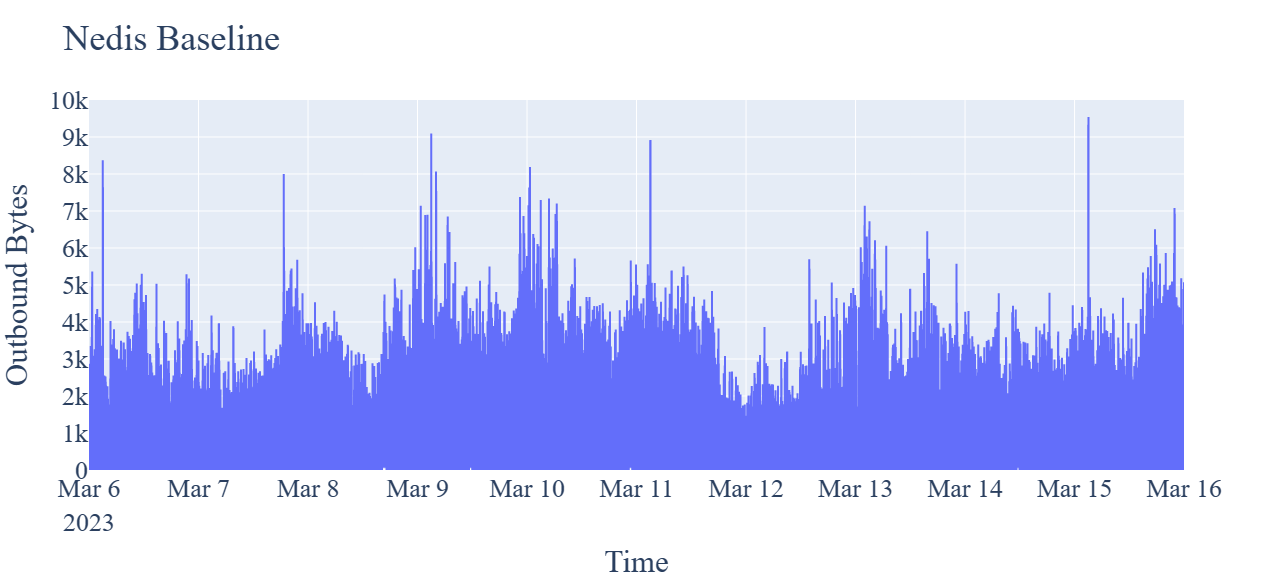
\includegraphics[width=\textwidth]{figures/Nedis_Baseline_OutboundBytes.png}
        \caption{Nedis outbound bytes}
    \end{subfigure}
    \begin{subfigure}[b]{0.4\textwidth}
        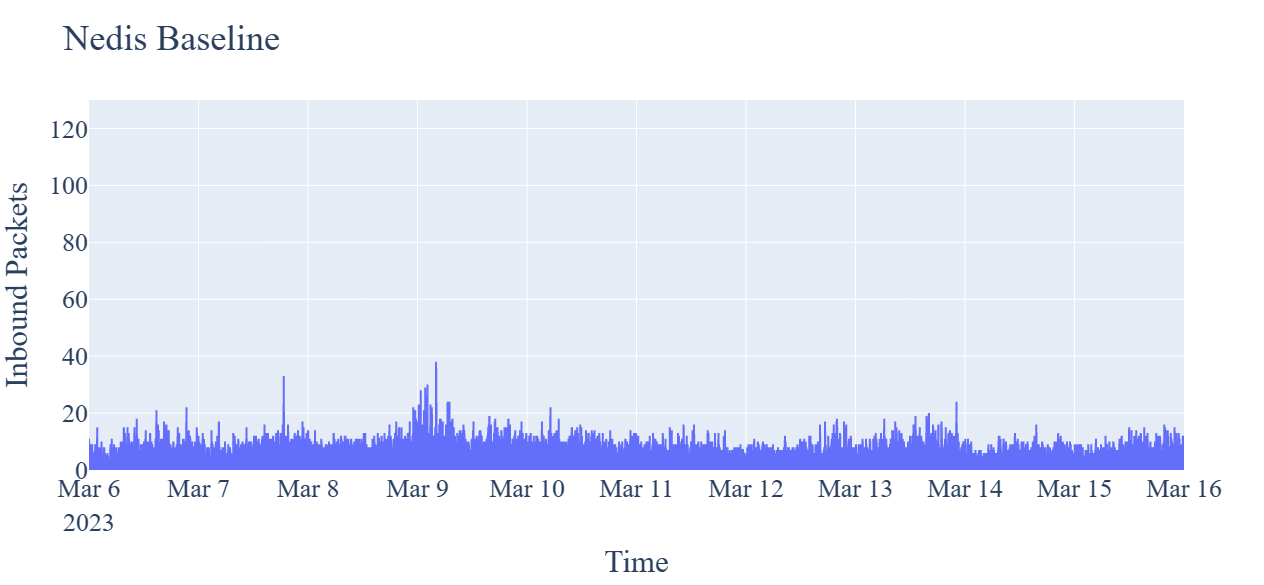
\includegraphics[width=\textwidth]{figures/Nedis_Baseline_InboundPackets.png}
        \caption{Nedis inbound packets}
    \end{subfigure}
    \begin{subfigure}[b]{0.4\textwidth}
        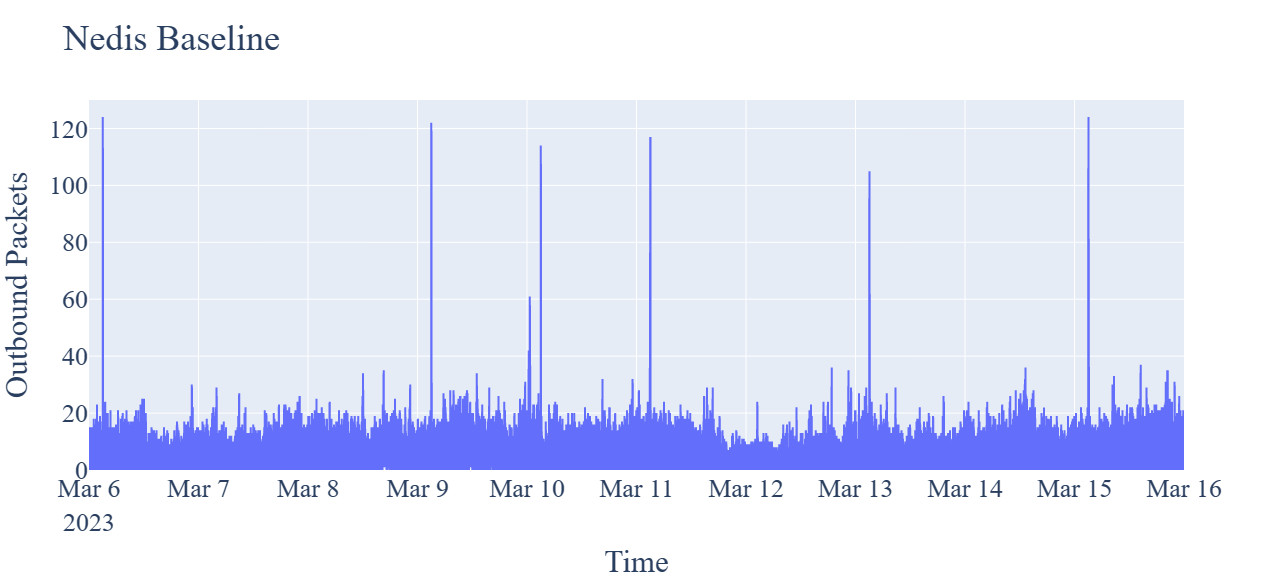
\includegraphics[width=\textwidth]{figures/Nedis_Baseline_OutboundPackets.png}
        \caption{Nedis outbound packets}
    \end{subfigure}
    \caption{Nedis baseline inbound and outbound bytes}
    \label{Fig:NedisBaselineOutandInboundTraffic}
 \end{figure}
 
\begin{table}[H]
    \caption{Calculations for Nedis baseline capture}
    \centering
    \begin{tabular}{ll|l|}
        \cline{3-3}                                               &                               &             \textbf{Numbers} \\ \hline
        \multicolumn{1}{|c|}{\multirow{4}{*}{\textbf{Total}}}    & Packets              & 2,428,701         \\ \cline{2-3} 
        \multicolumn{1}{|c|}{}                                   & Bytes                & 295,022,494       \\ \cline{2-3} 
        \multicolumn{1}{|c|}{}                                   & Average bytes/second & 341               \\ \cline{2-3} 
        \multicolumn{1}{|c|}{}                                   & Average packet size  & 121 bytes        \\ \hline
        \multicolumn{1}{|l|}{\multirow{5}{*}{\textbf{Inbound}}}  & Packets              & 451,495           \\ \cline{2-3} 
        \multicolumn{1}{|l|}{}                                   & Bytes                & 88,595,049        \\ \cline{2-3} 
        \multicolumn{1}{|l|}{}                                   & Average bytes/second & 102                \\ \cline{2-3} 
        \multicolumn{1}{|l|}{}                                   & Average packet size  & 196 bytes         \\ \cline{2-3} 
        \multicolumn{1}{|l|}{}                                   & Biggest packet       & 522 bytes        \\ \hline
        \multicolumn{1}{|l|}{\multirow{5}{*}{\textbf{Outbound}}} & Packets              & 1,977,206         \\ \cline{2-3} 
        \multicolumn{1}{|l|}{}                                   & Bytes                & 206,427,445      \\ \cline{2-3} 
        \multicolumn{1}{|l|}{}                                   & Average bytes/second & 238               \\ \cline{2-3} 
        \multicolumn{1}{|l|}{}                                   & Average packet size  & 104 bytes         \\ \cline{2-3} 
        \multicolumn{1}{|l|}{}                                   & Biggest packet       & 485 bytes       \\ \hline
    \end{tabular}
    \label{tab:NedisBaselineCalculations}
\end{table} 

To look at the differences in inbound and outbound traffic for Nedis, Figure \ref{Fig:NedisBaselineOutandInboundTraffic} are displayed. Figure \ref{Fig:NedisBaselineOutandInboundTraffic} shows that the spikes are packets which the device receives. Even though the graphs for inbound and outbound traffic from Nedis can look similar, the calculations presented in Table \ref{tab:NedisBaselineCalculations}, shows that 81\% of the packets and 70\% of the bytes in the baseline are traffic sent from the device. Looking at the graphs in total will therefore give the most to analyze. Another aspect of looking at the graphs in total, compared to inbound and outbound separately is that since the traffic is encrypted on the layer 2, it is not possible to know what makes the possible changes. 

\subsection{Summarizing and comparison}
This subsection summarizes and compares the baseline traffic for all the three devices. Table \ref{tab:ComparingBaselineCalculations} shows the differences in packets and bytes sent and received to each devices during the baseline capture. As the table shows, they send different amounts of packets and bytes. Nedis sends the most while Netatmo sends the least amount in standby. For inbound and outbound traffic, Netatmo and Nedis sends more packets than it receives, while Mill receives more packets than it sends. The same is shown in Figure \ref{fig:ComparingBaselines} for the total number of bytes and packets, in Figure \ref{Fig:CompareBaselineOutandInboundBytes} for inbound traffic and in Figure \ref{Fig:CompareBaselineOutandInboundPackets} for outbound traffic.

\begin{table}[H]
    \centering
    \caption{Comparing baseline calculations for all devices}
    \begin{tabular}{ll|l|l|l|}
    \cline{3-5}
                                                         &         & \textbf{Netatmo} & \textbf{Mill} & \textbf{Nedis} \\ \hline
        \multicolumn{1}{|l|}{\multirow{2}{*}{\textbf{Total}}}    & Packets & 110,735          & 1,236,753     & 2,428,701      \\ \cline{2-5} 
        \multicolumn{1}{|l|}{}                                   & Bytes   & 14,959,396       & 129,253,290   & 295,022,494    \\ \hline
        \multicolumn{1}{|l|}{\multirow{2}{*}{\textbf{Inbound}}}  & Packets & 1,042            & 942,112       & 451,495        \\ \cline{2-5} 
        \multicolumn{1}{|l|}{}                                   & Bytes   & 83,446           & 95,458,773    & 88,595,049     \\ \hline
        \multicolumn{1}{|l|}{\multirow{2}{*}{\textbf{Outbound}}} & Packets & 109,693          & 294,640       & 1,977,206      \\ \cline{2-5} 
        \multicolumn{1}{|l|}{}                                   & Bytes   & 14,875,950       & 33,794,517    & 206,427,445    \\ \hline
    \end{tabular}
    \label{tab:ComparingBaselineCalculations}
\end{table}
 
\begin{figure}[H]
    \centering
    \begin{subfigure}[b]{0.4\textwidth}
        \centering
        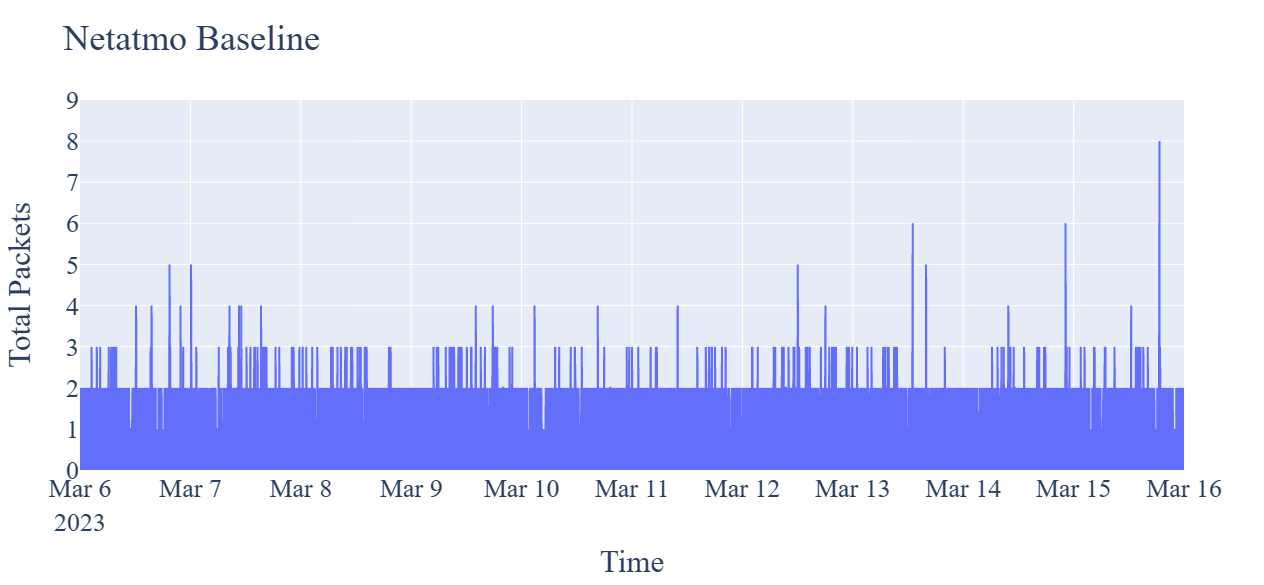
\includegraphics[width=1\hsize]{figures/Netatmo_Baseline_TotalPackets.png}
        \caption{Netatmo packets}
    \end{subfigure}
    \begin{subfigure}[b]{0.4\textwidth}
        \centering
        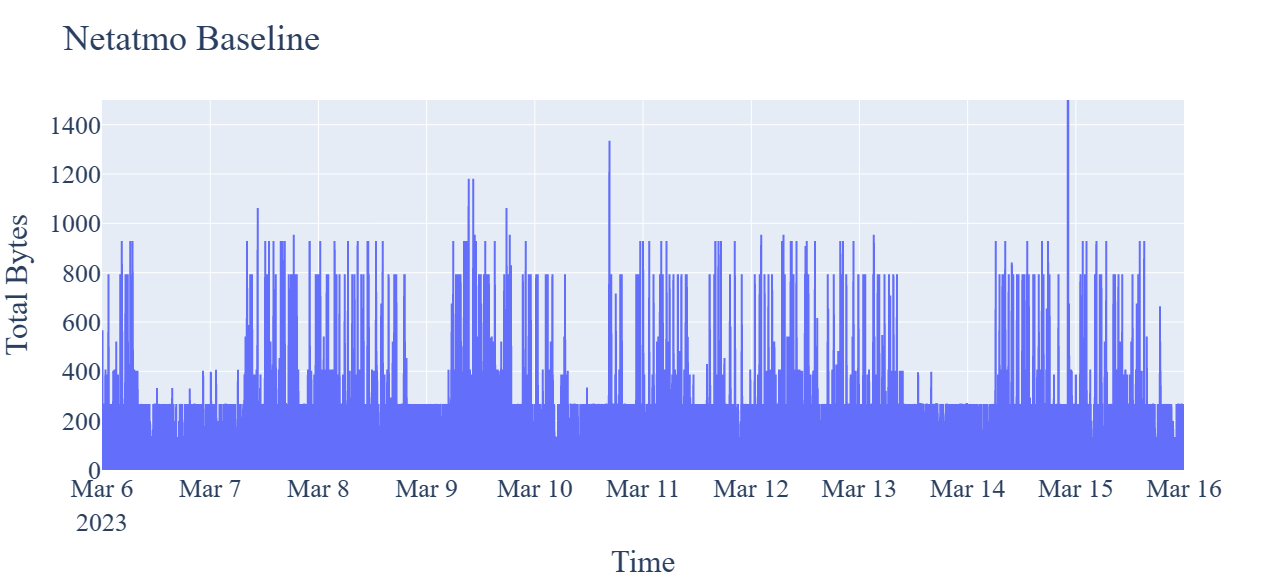
\includegraphics[width=1\hsize]{figures/Netatmo_Baseline_TotalBytes.png}
        \caption{Netatmo bytes}
    \end{subfigure}
    \begin{subfigure}[b]{0.4\textwidth}
        \centering
        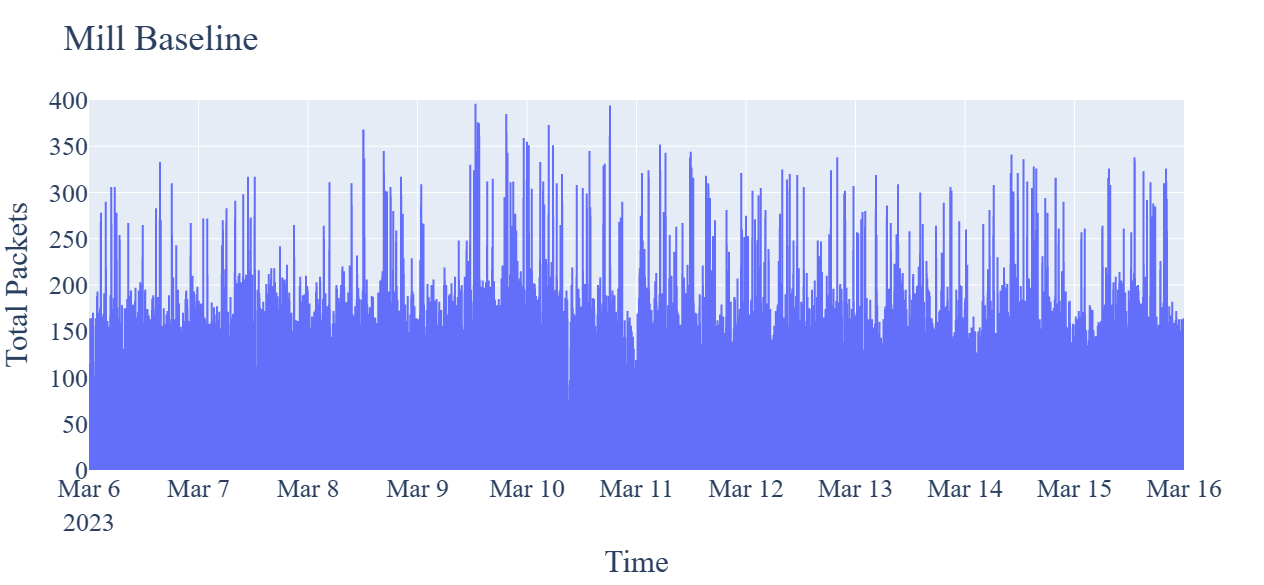
\includegraphics[width=1\hsize]{figures/Mill_Baseline_TotalPackets.png}
        \caption{Mill packets}
    \end{subfigure}
    \begin{subfigure}[b]{0.4\textwidth}
        \centering
        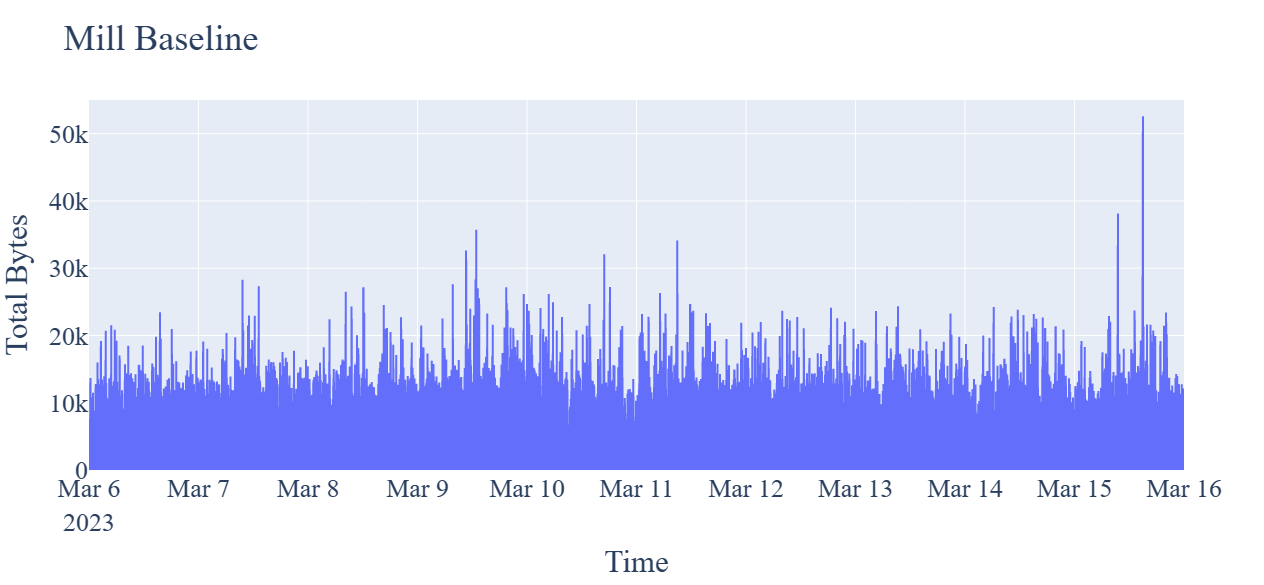
\includegraphics[width=1\hsize]{figures/Mill_Baseline_TotalBytes.png}
        \caption{Mill bytes}
    \end{subfigure}
    \begin{subfigure}[b]{0.4\textwidth}
        \centering
        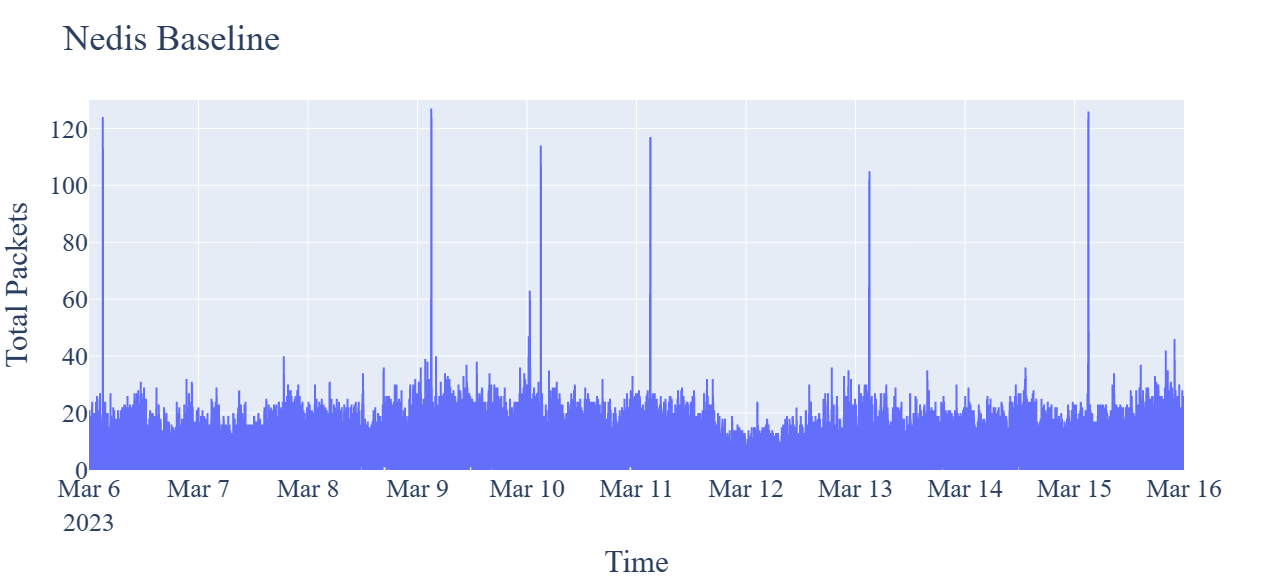
\includegraphics[width=1\hsize]{figures/Nedis_Baseline_TotalPackets.png}
        \caption{Nedis packets}
    \end{subfigure}
    \begin{subfigure}[b]{0.4\textwidth}
        \centering
        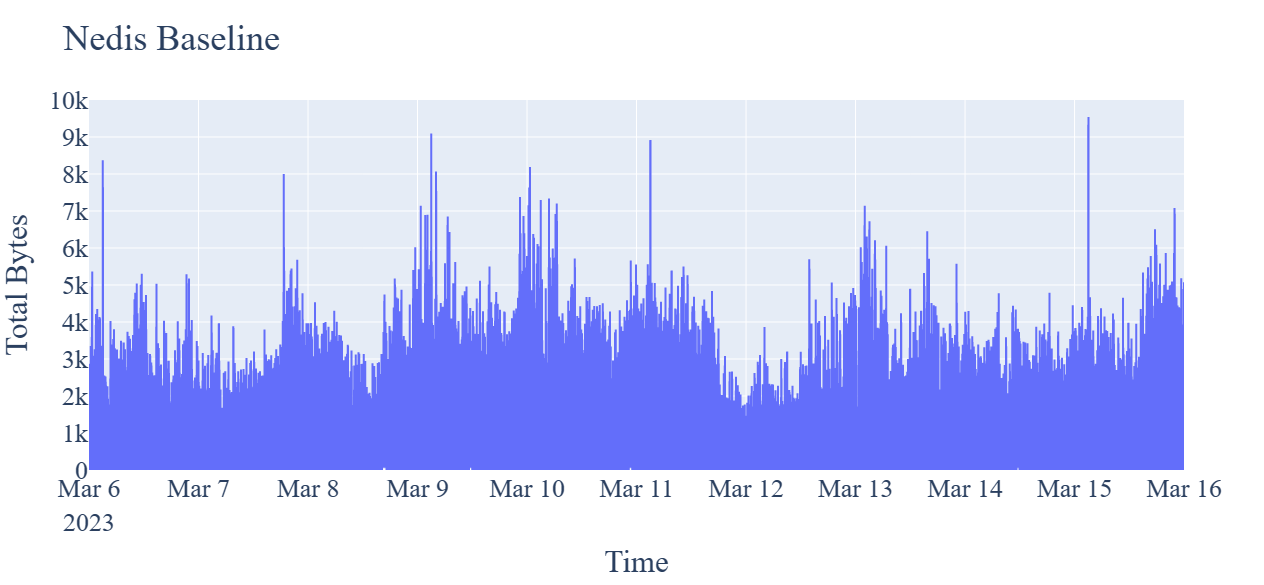
\includegraphics[width=1\hsize]{figures/Nedis_Baseline_TotalBytes.png}
        \caption{Nedis bytes}
    \end{subfigure}
    \caption{Comparing baseline graphs with total number of packets and bytes}
    \label{fig:ComparingBaselines}
\end{figure}

\begin{figure}[H]
    \centering
    \begin{subfigure}[b]{0.4\textwidth}
        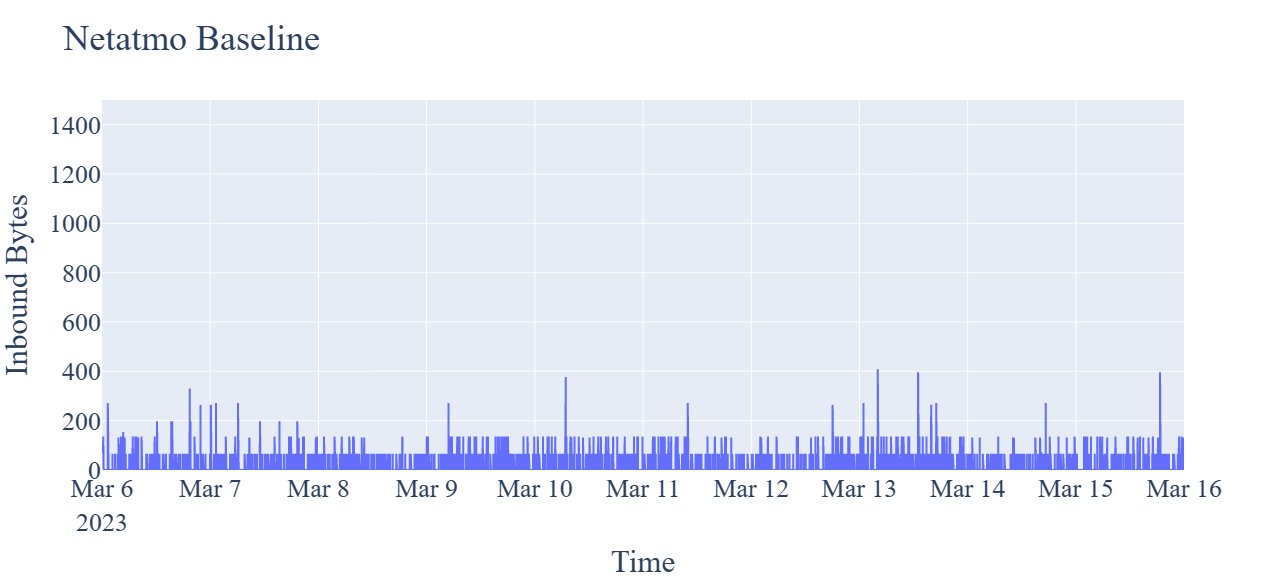
\includegraphics[width=\textwidth]{figures/Netatmo_Baseline_InboundBytes.png}
        \caption{Netatmo inbound bytes}
    \end{subfigure}
    \begin{subfigure}[b]{0.4\textwidth}
        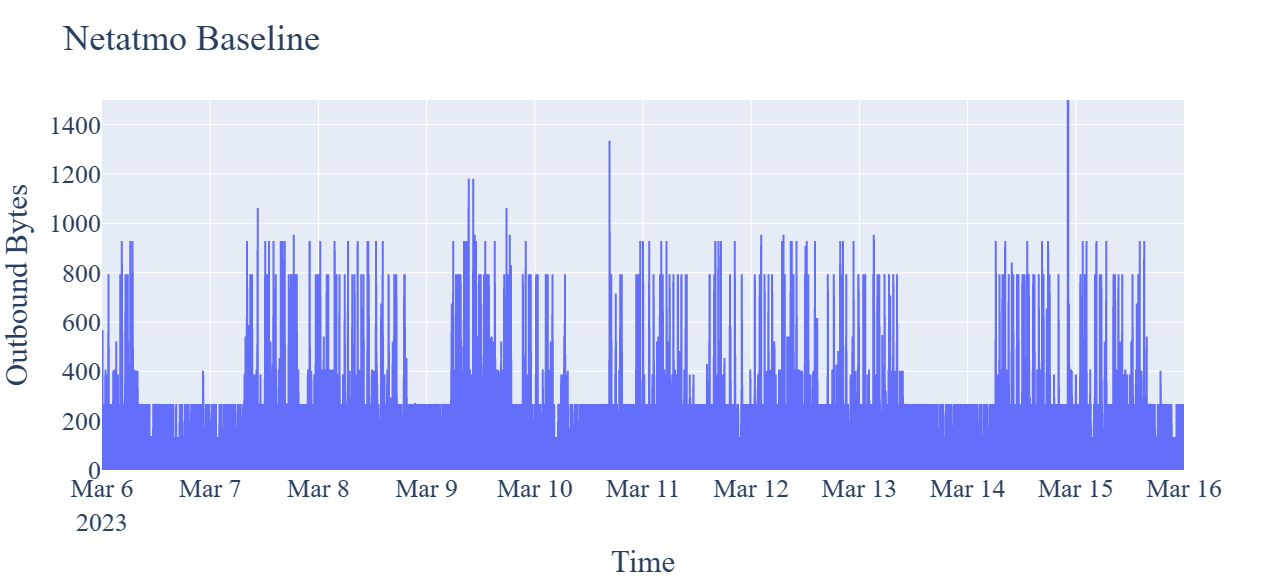
\includegraphics[width=\textwidth]{figures/Netatmo_Baseline_OutboundBytes.png}
        \caption{Netatmo outbound bytes}
    \end{subfigure}
    \begin{subfigure}[b]{0.4\textwidth}
        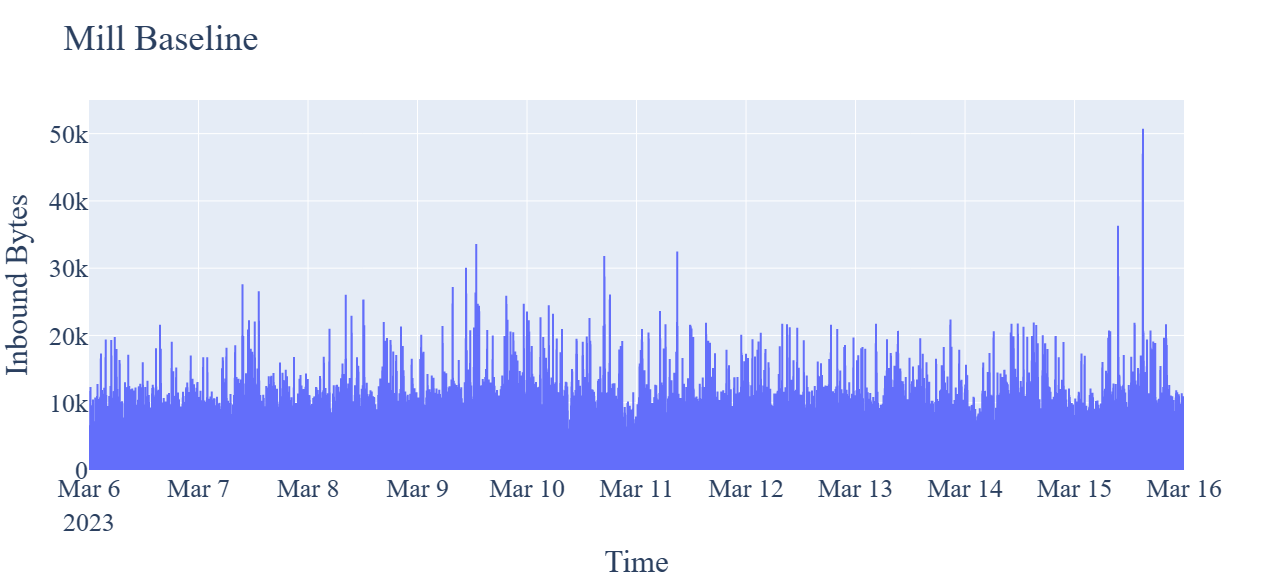
\includegraphics[width=\textwidth]{figures/Mill_Baseline_InboundBytes.png}
        \caption{Mill inbound bytes}
    \end{subfigure}
    \begin{subfigure}[b]{0.4\textwidth}
        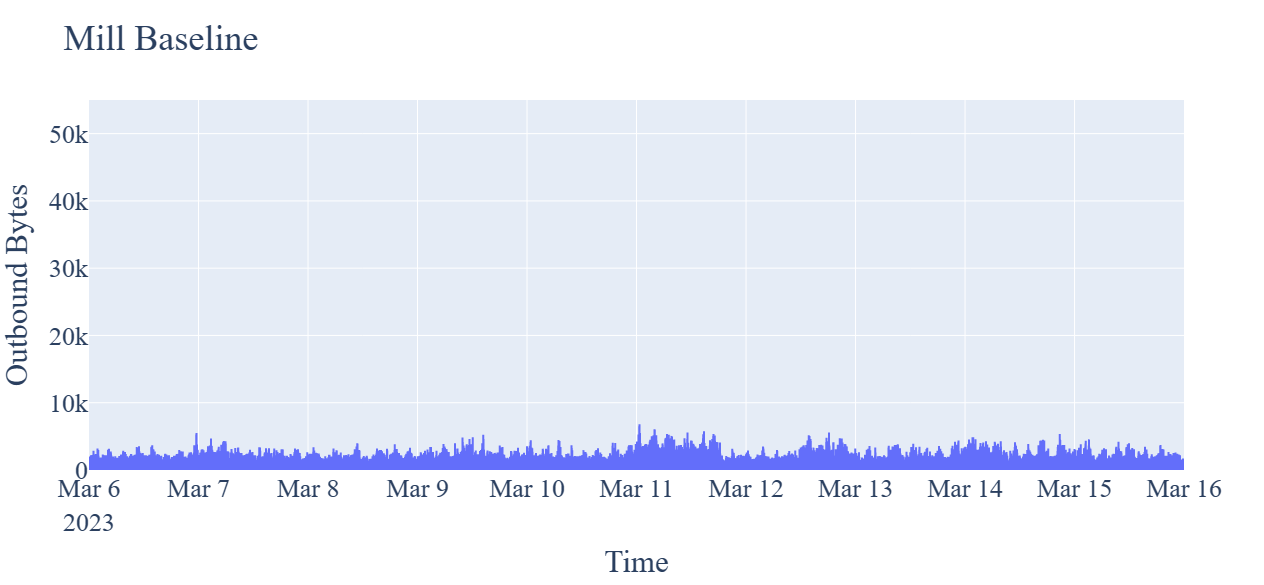
\includegraphics[width=\textwidth]{figures/Mill_Baseline_OutboundBytes.png}
        \caption{Mill outbound bytes}
    \end{subfigure}
    \begin{subfigure}[b]{0.4\textwidth}
        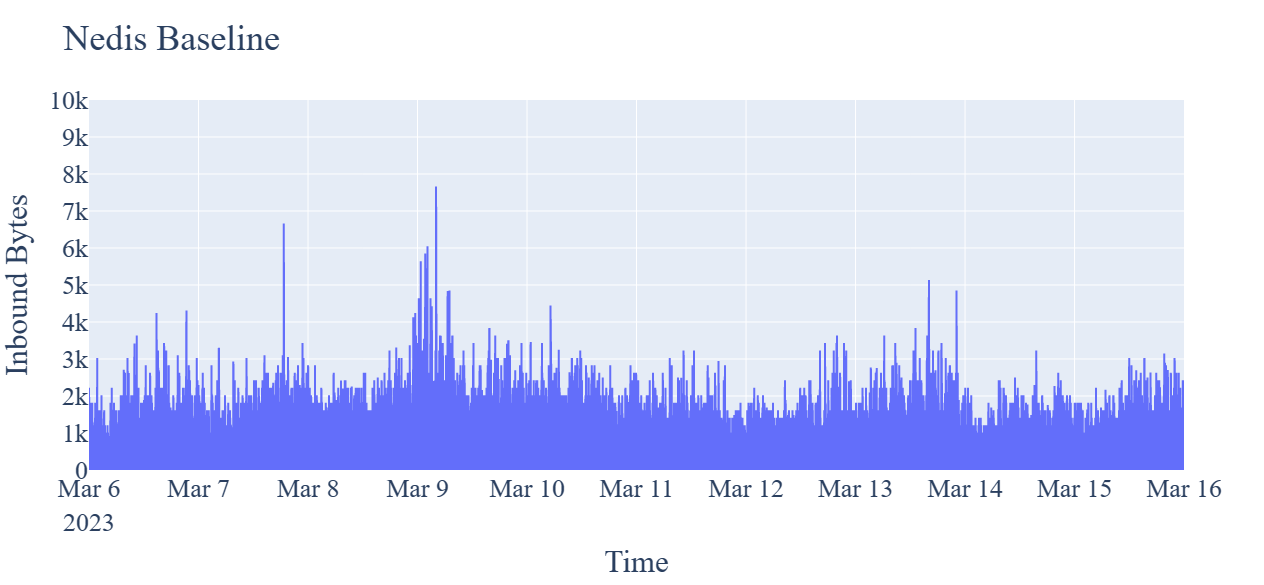
\includegraphics[width=\textwidth]{figures/Nedis_Baseline_InboundBytes.png}
        \caption{Nedis inbound bytes}
    \end{subfigure}
    \begin{subfigure}[b]{0.4\textwidth}
        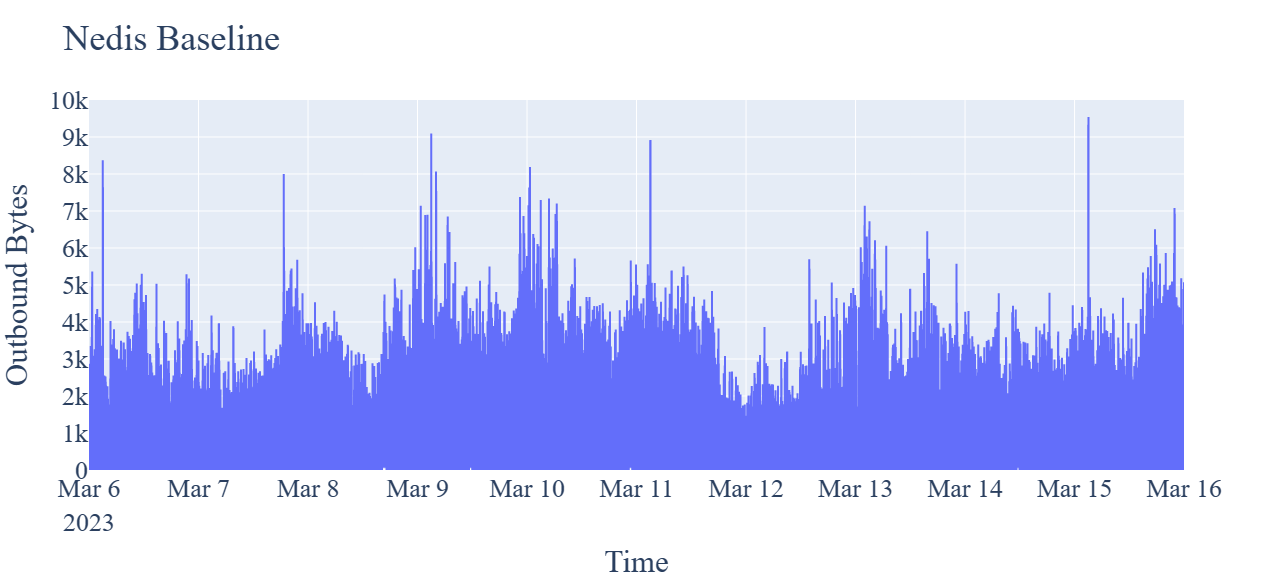
\includegraphics[width=\textwidth]{figures/Nedis_Baseline_OutboundBytes.png}
        \caption{Nedis outbound bytes}
    \end{subfigure}
    \caption{Comparing inbound and outbound bytes during baseline capture}
    \label{Fig:CompareBaselineOutandInboundBytes}
 \end{figure}

\begin{figure}[H]
    \centering
    \begin{subfigure}[b]{0.4\textwidth}
        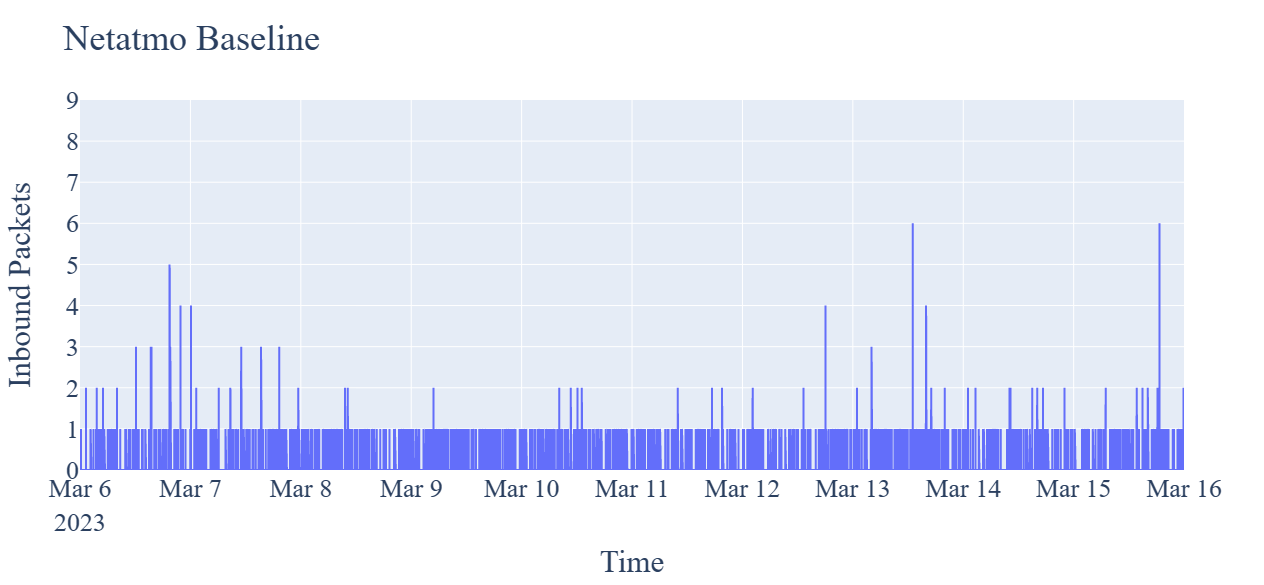
\includegraphics[width=\textwidth]{figures/Netatmo_Baseline_InboundPackets.png}
        \caption{Netatmo inbound packets}
    \end{subfigure}
    \begin{subfigure}[b]{0.4\textwidth}
        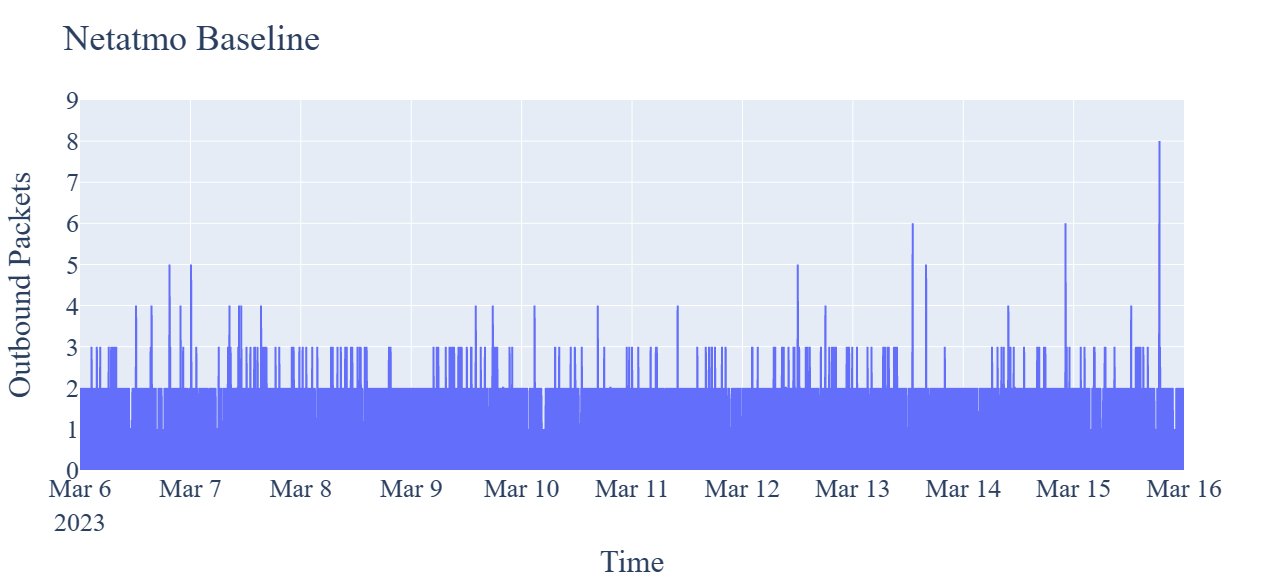
\includegraphics[width=\textwidth]{figures/Netatmo_Baseline_OutboundPackets.png}
        \caption{Netatmo outbound packets}
    \end{subfigure}
    \begin{subfigure}[b]{0.4\textwidth}
        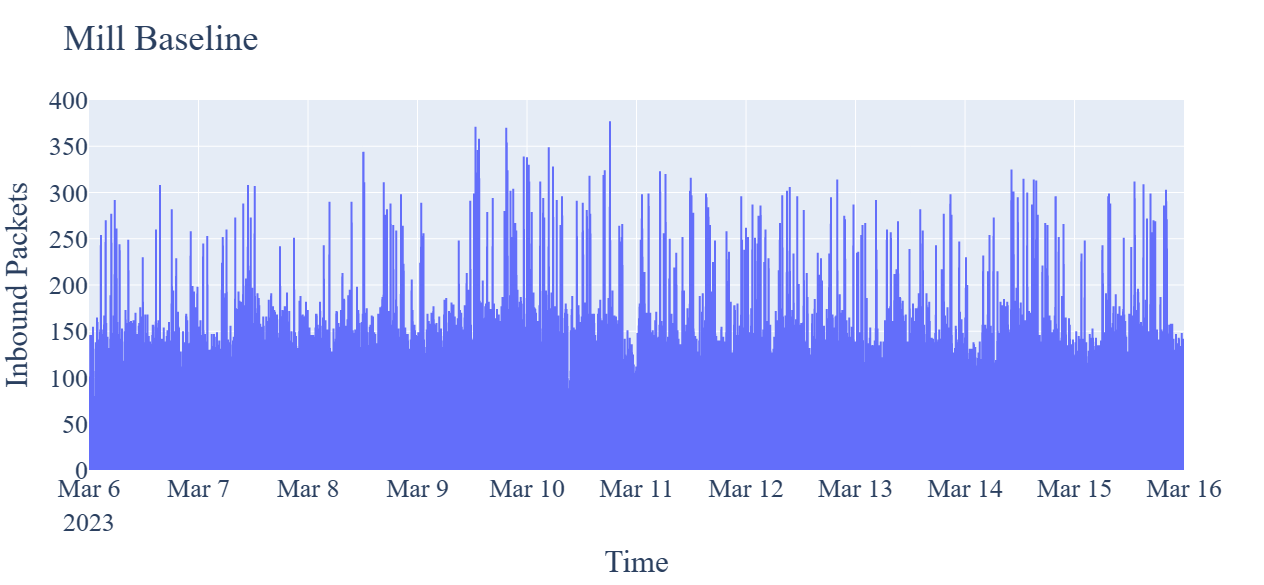
\includegraphics[width=\textwidth]{figures/Mill_Baseline_InboundPackets.png}
        \caption{Mill inbound packets}
    \end{subfigure}
    \begin{subfigure}[b]{0.4\textwidth}
        \includegraphics[width=\textwidth]{figures/Mill_Baseline_outboundPackets.png}
        \caption{Mill outbound packets}
    \end{subfigure}
    \begin{subfigure}[b]{0.4\textwidth}
        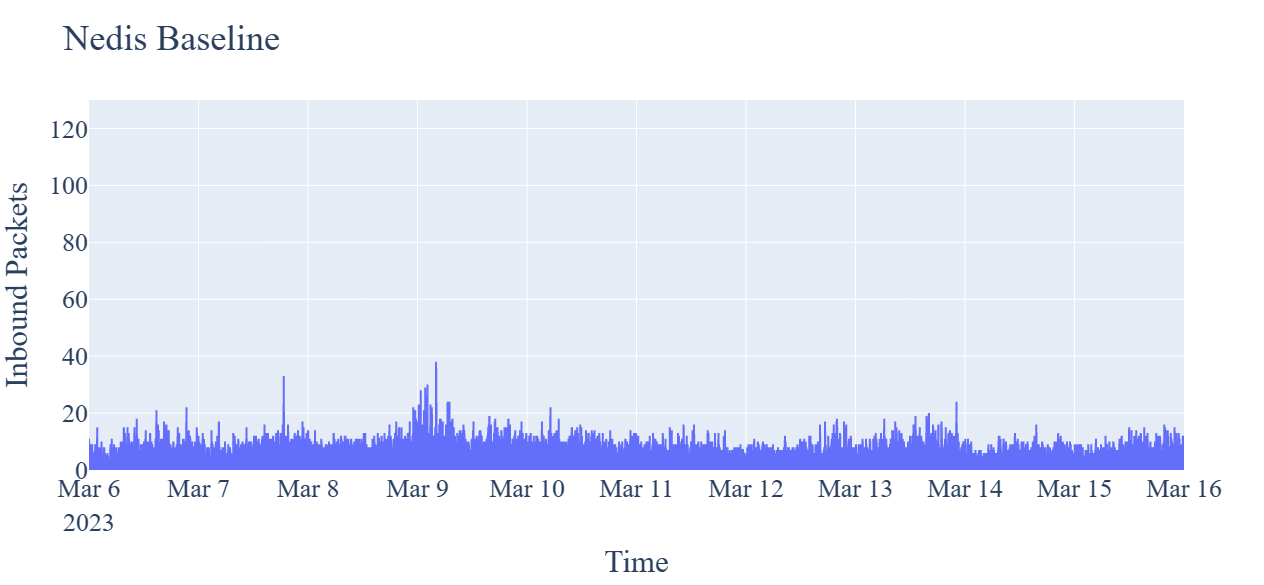
\includegraphics[width=\textwidth]{figures/Nedis_Baseline_InboundPackets.png}
        \caption{Nedis inbound Packets}
    \end{subfigure}
    \begin{subfigure}[b]{0.4\textwidth}
        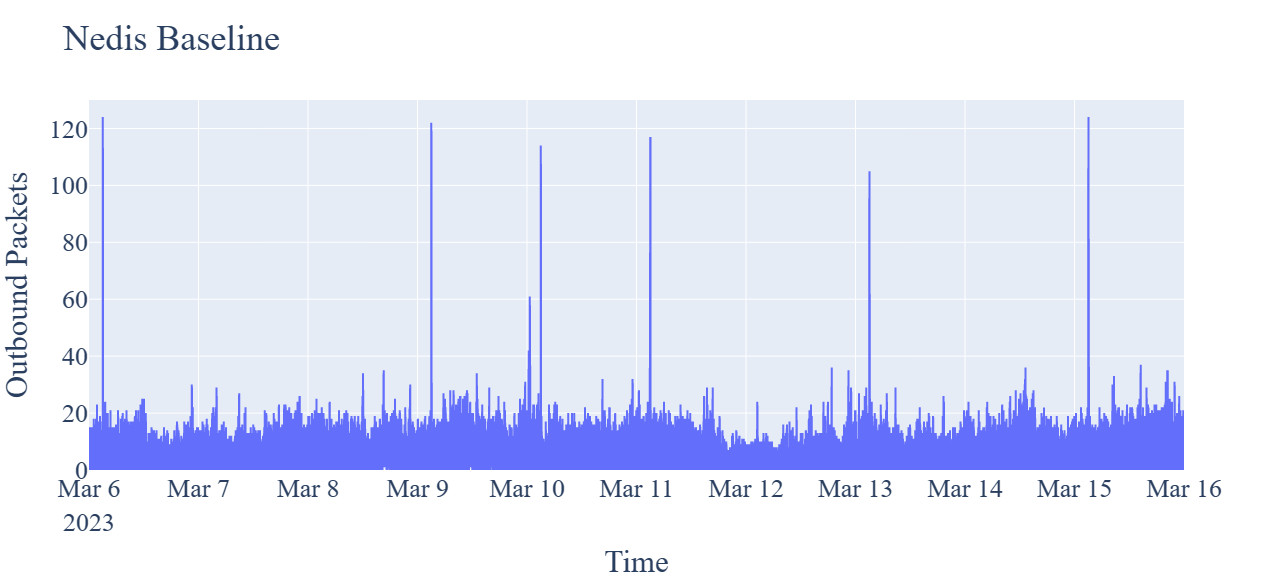
\includegraphics[width=\textwidth]{figures/Nedis_Baseline_OutboundPackets.png}
        \caption{Nedis outbound packets}
    \end{subfigure}
    \caption{Comparing inbound and outbound packets during baseline capture}
    \label{Fig:CompareBaselineOutandInboundPackets}
 \end{figure}

\newpage
\section{Test Case 1: Cooking}
This chapter presents the results and analysis conducted on Test Case 1: Cooking. The first subsection will present general information applicable to all the devices, and the following subsections will present the result and analysis for each of the devices separately. 
\subsection{General}
The cooking events are 10 in total and are presented in Table \ref{tab:CookingDates}. Every device has the same time and dates for this event. 
\begin{table}[H]
    \centering
    \caption{Date and time for Test Case 1: Cooking Events}
    \begin{adjustbox}{width=1\textwidth}
            \begin{tabular}{l|l|l|l|l|l|l|l|l|l|l|}
            \cline{2-11} & 08.01 & 09.01 & 11.01 & 16.01 & 18.01 & 19.01 & 25.01 & 30.01 & 31.01 & 01.02 \\
            \hline
            \multicolumn{1}{|l|}{Started event}  & 15:58 & 15:59 & 16:05 & 16:02 & 16:04 & 16:01 & 16:02 & 16:01 & 16:01 & 16:02 \\ 
            \hline
            \multicolumn{1}{|l|}{Finished event} & 16:22 & 16:21 & 16:37 & 16:25 & 16:25 & 16:18 & 16:13 & 16:19 & 16:21 & 16:22 \\ \hline
            \end{tabular}
    \end{adjustbox}
    \label{tab:CookingDates}
\end{table}
\FloatBarrier

To be able to look even further into if it is a similar traffic pattern to each event that can be used to identify it, the same start and finish time will be used for every graph. To have the same amount of time on each event the earliest start time and the latest finish time are used as filtering values for each of the pcaps to be used in analyzing the cooking event. These values were then added 30 minutes before and after and used as a the start and finish time for the events, while the actual event time given by Table \ref{tab:CookingDates} are marked red on the graphs. This gives the following values to use for further analysis:

\begin{itemize}
    \item Earliest Event Start: 15:58
    \item Latest Event Finished: 16:37
    \item Packet Capture Files Start: 15:28
    \item Packet Capture Files End: 17:07
\end{itemize}

These timings gives the following filters added to create the pcaps for each event:

\begin{itemize}
    \item frame.time >= "Month Date, Year 15:28:00" \&\& frame.time <= "Month Date, Year 17:07:00"
\end{itemize}

\newpage
\subsection{Netatmo}
Table \ref{tab:NetatmoCookingCalculations} presents calculations from all the cooking events together with a standard deviation and Table \ref{tab:NetatmoBaselineCookingCalculations} presents the calculations from all the corresponding baseline pcaps. Table \ref{tab:NetatmoComparingBaselineAndCookingCalculations} compares the average and standard deviation values from the events to the baseline. Figure \ref{fig:NetatmoCookingCalculations} presents a graphical overview of the packets and bytes from Table \ref{tab:NetatmoCookingCalculations} including average values.

\begin{table}[H]
    \centering
    \caption{Netatmo event calculations for the cooking events}
    \begin{tabular}{|l|l|l|l|l|l|}
    \hline
        \textbf{Event dates} & \textbf{Packets} & \textbf{Bytes} & \textbf{Biggest packet} \\ \hline
        08.jan & 901 & 123,630 & 407 bytes\\ \hline
        09.jan & 703 & 97,019 & 407 bytes \\ \hline
        11.jan & 847 & 114,473 & 407 bytes\\ \hline
        16.jan & 1,082 & 146,001 & 407 bytes\\ \hline
        18.jan & 948 & 129,907 & 407 bytes\\ \hline
        19.jan & 828 & 111,629 & 407 bytes \\ \hline
        25.jan & 430 & 58,926 & 407 bytes \\ \hline
        30.jan & 815 & 110,838 & 407 bytes \\ \hline
        31.jan & 864 & 115,302 & 136 bytes \\ \hline
        01.feb & 805 & 109,050 & 407 bytes \\ \hline
    \end{tabular}
    \label{tab:NetatmoCookingCalculations}
\end{table}

\begin{table}[!ht]
    \centering
    \caption{Netatmo baseline calculations for the corresponding cooking event times}
    \begin{tabular}{|l|l|l|l|}
    \hline
        \textbf{Baseline} & \textbf{Packets} & \textbf{Bytes} & \textbf{Biggest packet} \\ \hline
        06.mar & 584 & 77,780 & 134 bytes\\ \hline
        07.mar & 972 & 132,406 & 407 bytes\\ \hline
        08.mar & 697 & 94,730 & 407 bytes \\ \hline
        09.mar & 868 & 117,020 & 407 bytes \\ \hline
        10.mar & 825 & 111,863 & 407 bytes \\ \hline
        11.mar & 745 & 101,534 & 407 bytes \\ \hline
        12.mar & 626 & 84,987 & 407 bytes \\ \hline
        13.mar & 764 & 101,772 & 136 bytes \\ \hline
        14.mar & 750 & 102,396 & 407 bytes \\ \hline
        15.mar & 812 & 108,703 & 407 bytes \\ \hline
    \end{tabular}
    \label{tab:NetatmoBaselineCookingCalculations}
\end{table}

\begin{table}[H]
    \centering
    \caption{Netatmo: Comparing event and baseline calculations for the cooking test}
    \begin{tabular}{c|l|l|l|l|}
        \cline{2-5}
        \multicolumn{1}{l|}{}                                              & \textbf{Type} & \textbf{Packets} & \textbf{Bytes} & \textbf{Biggest packet} \\ \hline
        \multicolumn{1}{|c|}{\multirow{2}{*}{\textbf{Average}}}            & Event         & 822              & 111,678        & 380 bytes               \\ \cline{2-5} 
        \multicolumn{1}{|c|}{}                                             & Baseline      & 764              & 103,319        & 353 bytes                \\ \hline
        \multicolumn{1}{|c|}{\multirow{2}{*}{\textbf{Standard deviation}}} & Event         & 170              & 22,802         & 86 bytes                 \\ \cline{2-5} 
        \multicolumn{1}{|c|}{}                                             & Baseline      & 114              & 15,650         & 115 bytes               \\ \hline          
    \end{tabular}
    \label{tab:NetatmoComparingBaselineAndCookingCalculations}
\end{table}

\begin{figure}[H]
    \centering
    \begin{subfigure}{0.8\textwidth}
       \centering
       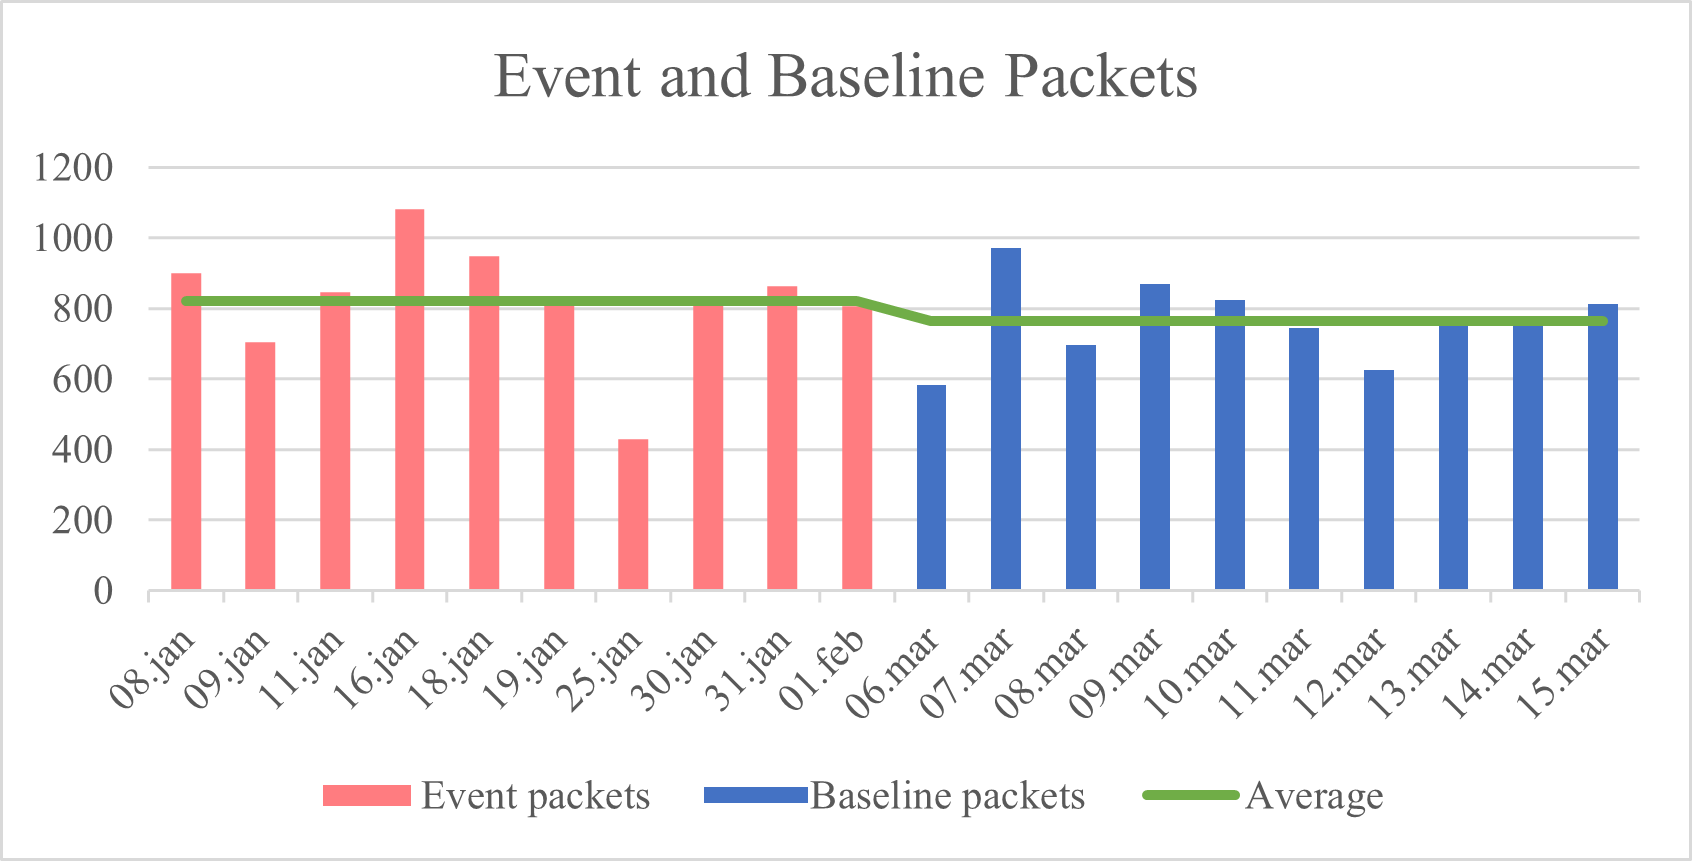
\includegraphics[width=1\hsize]{figures/Netatmo_Cooking_Calculations_Packets.png} 
    \end{subfigure}
    \begin{subfigure}{0.8\textwidth}
        \centering
        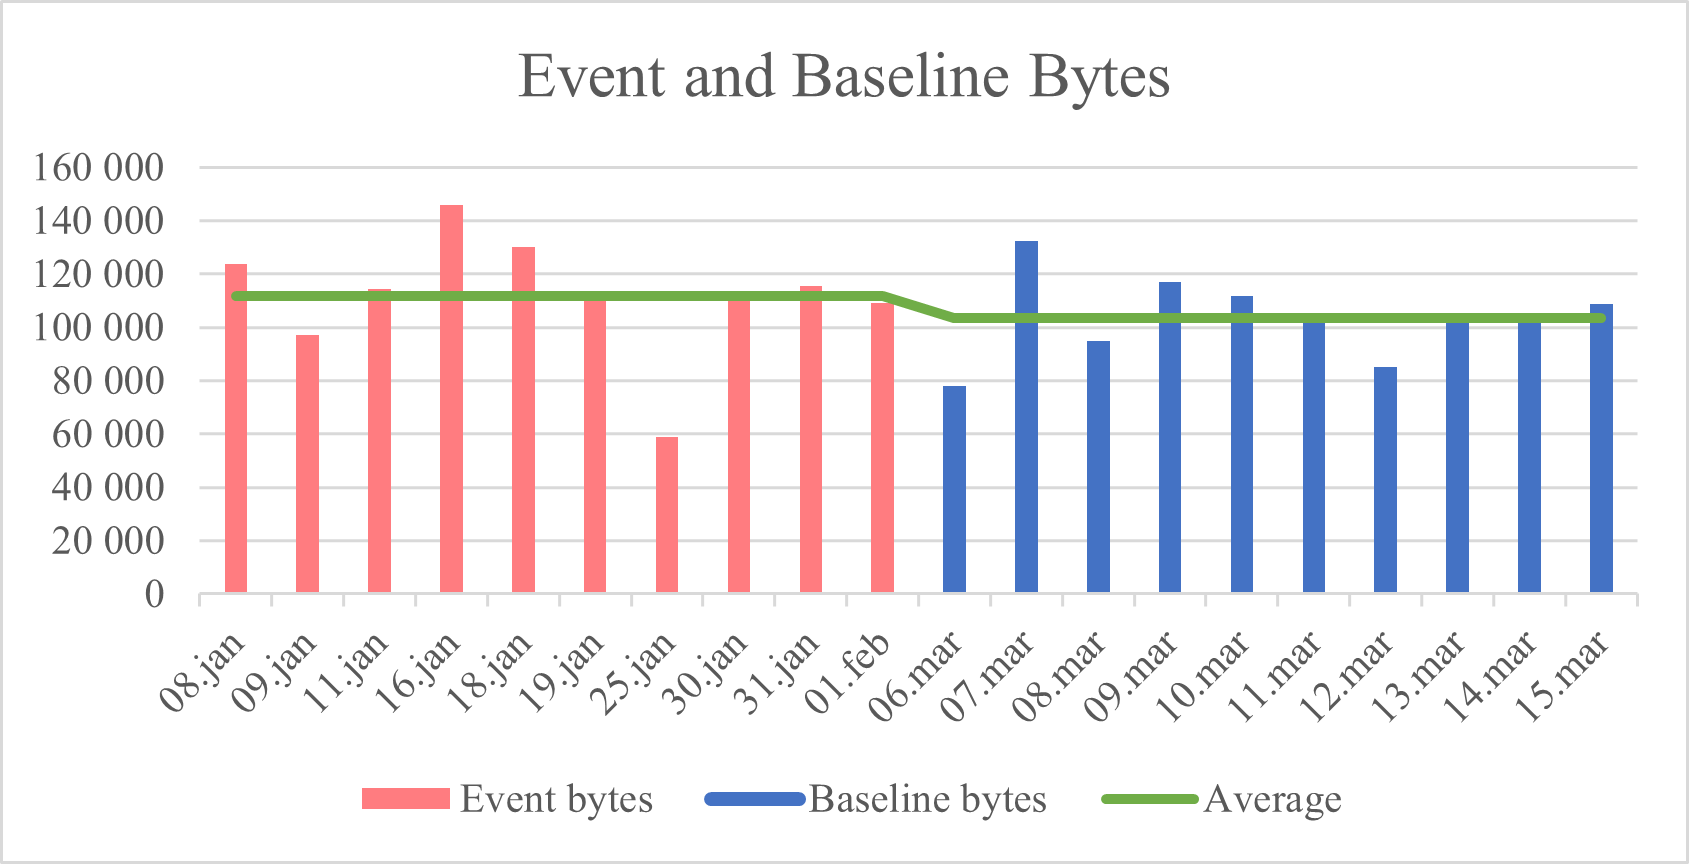
\includegraphics[width=1\hsize]{figures/Netatmo_Cooking_Calculations_Bytes.png} 
    \end{subfigure}
    \caption{Netatmo: Graphical presentation of event and baseline cooking calculations with packets and bytes, including average value extracted from Table \ref{tab:NetatmoCookingCalculations}}
    \label{fig:NetatmoCookingCalculations}
\end{figure}

The graphs in Figure \ref{fig:NetatmoCookingBytes1}, \ref{fig:NetatmoCookingBytes2}, \ref{fig:NetatmoCookingPackets1} and \ref{fig:NetatmoCookingPackets2} displays both bytes and packets for the cooking events in comparison with the baseline captures. The event graphs are placed on the left side of the figure and are framed in red, the baseline graphs are placed on the right side of the figure and are framed in blue. The area marked red on the event graphs are when the event was ongoing, and not included in the baseline graphs as no event was ongoing and is only used for comparison. The x- and y-axis for all the graphs in the same figure have the same minimum and maximum values. 

\begin{figure}[H]
    \begin{subfigure}[b]{0.47\textwidth}
        \centering
        \tcbincludegraphics[size=fbox,width=1.1\hsize,colframe=red]{figures/Netatmo_Cooking_Packets_08.01.png}
    \end{subfigure}
    \begin{subfigure}[b]{0.47\textwidth}
        \centering
        \tcbincludegraphics[size=fbox,width=1.1\hsize, colframe=blue]{figures/Netatmo_Cooking_Baseline_Packets_06.03.png}
    \end{subfigure}
    \begin{subfigure}[b]{0.47\textwidth}
        \centering
        \tcbincludegraphics[size=fbox,width=1.1\hsize,colframe=red]{figures/Netatmo_Cooking_Packets_09.01.png}
    \end{subfigure}
    \begin{subfigure}[b]{0.47\textwidth}
        \centering
        \tcbincludegraphics[size=fbox,width=1.1\hsize,colframe=blue]{figures/Netatmo_Cooking_Baseline_Packets_07.03.png}
    \end{subfigure}
    \begin{subfigure}[b]{0.47\textwidth}
        \centering
        \tcbincludegraphics[size=fbox,width=1.1\hsize,colframe=red]{figures/Netatmo_Cooking_Packets_11.01.png}
    \end{subfigure}
    \begin{subfigure}[b]{0.47\textwidth}
        \centering
        \tcbincludegraphics[size=fbox,width=1.1\hsize,colframe=blue]{figures/Netatmo_Cooking_Baseline_Packets_08.03.png}
    \end{subfigure}
    \begin{subfigure}[b]{0.47\textwidth}
        \centering
        \tcbincludegraphics[size=fbox,width=1.1\hsize,colframe=red]{figures/Netatmo_Cooking_Packets_16.01.png}
    \end{subfigure}
    \begin{subfigure}[b]{0.47\textwidth}
        \centering
        \tcbincludegraphics[size=fbox,width=1.1\hsize,colframe=blue]{figures/Netatmo_Cooking_Baseline_Packets_09.03.png}
    \end{subfigure}
    \begin{subfigure}[b]{0.47\textwidth}
        \centering
        \tcbincludegraphics[size=fbox,width=1.1\hsize,colframe=red]{figures/Netatmo_Cooking_Packets_18.01.png}
    \end{subfigure}
    \begin{subfigure}[b]{0.47\textwidth}
        \centering
        \tcbincludegraphics[size=fbox,width=1.1\hsize,colframe=blue]{figures/Netatmo_Cooking_Baseline_Packets_10.03.png}
    \end{subfigure}
        \begin{subfigure}[b]{0.47\textwidth}
        \centering
        \tcbincludegraphics[size=fbox,width=1.1\hsize,colframe=red]{figures/Netatmo_Cooking_Packets_19.01.png}
    \end{subfigure}
    \begin{subfigure}[b]{0.47\textwidth}
        \centering
        \tcbincludegraphics[size=fbox,width=1.1\hsize,colframe=blue]{figures/Netatmo_Cooking_Baseline_Packets_11.03.png}
    \end{subfigure}
    \begin{subfigure}[b]{0.47\textwidth}
        \centering
        \tcbincludegraphics[size=fbox,width=1.1\hsize,colframe=red]{figures/Netatmo_Cooking_Packets_25.01.png}
    \end{subfigure}
    \hspace{0.6cm}
    \begin{subfigure}[b]{0.47\textwidth}
    \centering
        \tcbincludegraphics[size=fbox,width=1.1\hsize,colframe=blue]{figures/Netatmo_Cooking_Baseline_Packets_12.03.png}
        \end{subfigure}
    \caption{Netatmo: Graphs of traffic flows from the cooking events measured in packets with event graphs framed in red and baseline graphs framed in blue, Event times are marked in red on the event graphs.}
    \label{fig:NetatmoCookingPackets1}
\end{figure}

\begin{figure}[H]
    \begin{subfigure}[b]{0.45\textwidth}
        \centering
        \tcbincludegraphics[size=fbox,width=1.1\hsize,colframe=red]{figures/Netatmo_Cooking_Packets_30.01.png}
    \end{subfigure}
    \begin{subfigure}[b]{0.45\textwidth}
        \centering
        \tcbincludegraphics[size=fbox,width=1.1\hsize, colframe=blue]{figures/Netatmo_Cooking_Baseline_Packets_13.03.png}
    \end{subfigure}
    \begin{subfigure}[b]{0.45\textwidth}
        \centering
        \tcbincludegraphics[size=fbox,width=1.1\hsize,colframe=red]{figures/Netatmo_Cooking_Packets_31.01.png}
    \end{subfigure}
    \begin{subfigure}[b]{0.45\textwidth}
        \centering
        \tcbincludegraphics[size=fbox,width=1.1\hsize,colframe=blue]{figures/Netatmo_Cooking_Baseline_Packets_14.03.png}
    \end{subfigure}
    \begin{subfigure}[b]{0.45\textwidth}
        \centering
        \tcbincludegraphics[size=fbox,width=1.1\hsize,colframe=red]{figures/Netatmo_Cooking_Packets_01.02.png}
    \end{subfigure}
    \hspace{1.1cm}
    \begin{subfigure}[b]{0.45\textwidth}
        \centering
        \tcbincludegraphics[size=fbox,width=1.1\hsize,colframe=blue]{figures/Netatmo_Cooking_Baseline_Packets_15.03.png}
    \end{subfigure}
    \caption{Netatmo: Continuing from Figure \ref{fig:NetatmoCookingPackets1}}
    \label{fig:NetatmoCookingPackets2}
\end{figure}

\begin{figure}[H]
    \begin{subfigure}[b]{0.45\textwidth}
        \centering
        \tcbincludegraphics[size=fbox,width=1.1\hsize,colframe=red]{figures/Netatmo_Cooking_Bytes_30.01.png}
    \end{subfigure}
    \begin{subfigure}[b]{0.45\textwidth}
        \centering
        \tcbincludegraphics[size=fbox,width=1.1\hsize, colframe=blue]{figures/Netatmo_Cooking_Baseline_Bytes_13.03.png}
    \end{subfigure}
    \begin{subfigure}[b]{0.45\textwidth}
        \centering
        \tcbincludegraphics[size=fbox,width=1.1\hsize,colframe=red]{figures/Netatmo_Cooking_Bytes_31.01.png}
    \end{subfigure}
    \begin{subfigure}[b]{0.45\textwidth}
        \centering
        \tcbincludegraphics[size=fbox,width=1.1\hsize,colframe=blue]{figures/Netatmo_Cooking_Baseline_Bytes_14.03.png}
    \end{subfigure}
    \begin{subfigure}[b]{0.45\textwidth}
        \centering
        \tcbincludegraphics[size=fbox,width=1.1\hsize,colframe=red]{figures/Netatmo_Cooking_Bytes_01.02.png}
    \end{subfigure}
    \hspace{1.1cm}
    \begin{subfigure}[b]{0.45\textwidth}
        \centering
        \tcbincludegraphics[size=fbox,width=1.1\hsize,colframe=blue]{figures/Netatmo_Cooking_Baseline_Bytes_15.03.png}
    \end{subfigure}
    \caption{Netatmo: Remaining graphs from Figure \ref{fig:NetatmoCookingBytes2}}
    \label{fig:NetatmoCookingBytes1}
\end{figure}

\begin{figure}[H]
    \begin{subfigure}[b]{0.47\textwidth}
        \centering
        \tcbincludegraphics[size=fbox,width=1.1\hsize,colframe=red]{figures/Netatmo_Cooking_Bytes_08.01.png}
    \end{subfigure}
    \begin{subfigure}[b]{0.47\textwidth}
        \centering
        \tcbincludegraphics[size=fbox,width=1.1\hsize,colframe=blue]{figures/Netatmo_Cooking_Baseline_Bytes_06.03.png}
    \end{subfigure}
    \begin{subfigure}[b]{0.47\textwidth}
        \centering
        \tcbincludegraphics[size=fbox,width=1.1\hsize,colframe=red]{figures/Netatmo_Cooking_Bytes_09.01.png}
    \end{subfigure}
    \begin{subfigure}[b]{0.47\textwidth}
        \centering
        \tcbincludegraphics[size=fbox,width=1.1\hsize,colframe=blue]{figures/Netatmo_Cooking_Baseline_Bytes_07.03.png}
    \end{subfigure}
    \begin{subfigure}[b]{0.47\textwidth}
        \centering
        \tcbincludegraphics[size=fbox,width=1.1\hsize,colframe=red]{figures/Netatmo_Cooking_Bytes_11.01.png}
    \end{subfigure}
    \begin{subfigure}[b]{0.47\textwidth}
        \centering
        \tcbincludegraphics[size=fbox,width=1.1\hsize,colframe=blue]{figures/Netatmo_Cooking_Baseline_Bytes_08.03.png}
    \end{subfigure}
    \begin{subfigure}[b]{0.47\textwidth}
        \centering
        \tcbincludegraphics[size=fbox,width=1.1\hsize,colframe=red]{figures/Netatmo_Cooking_Bytes_16.01.png}
    \end{subfigure}
    \begin{subfigure}[b]{0.47\textwidth}
        \centering
        \tcbincludegraphics[size=fbox,width=1.1\hsize,colframe=blue]{figures/Netatmo_Cooking_Baseline_Bytes_09.03.png}
    \end{subfigure}
    \begin{subfigure}[b]{0.47\textwidth}
        \centering
        \tcbincludegraphics[size=fbox,width=1.1\hsize,colframe=red]{figures/Netatmo_Cooking_Bytes_18.01.png}
    \end{subfigure}
    \begin{subfigure}[b]{0.47\textwidth}
        \centering
        \tcbincludegraphics[size=fbox,width=1.1\hsize,colframe=blue]{figures/Netatmo_Cooking_Baseline_Bytes_10.03.png}
    \end{subfigure}
        \begin{subfigure}[b]{0.47\textwidth}
        \centering
        \tcbincludegraphics[size=fbox,width=1.1\hsize,colframe=red]{figures/Netatmo_Cooking_Bytes_19.01.png}
    \end{subfigure}
    \begin{subfigure}[b]{0.47\textwidth}
        \centering
        \tcbincludegraphics[size=fbox,width=1.1\hsize,colframe=blue]{figures/Netatmo_Cooking_Baseline_Bytes_11.03.png}
    \end{subfigure}
    \begin{subfigure}[b]{0.47\textwidth}
        \centering
        \tcbincludegraphics[size=fbox,width=1.1\hsize,colframe=red]{figures/Netatmo_Cooking_Bytes_25.01.png}
    \end{subfigure}
    \hspace{0.6cm}
    \begin{subfigure}[b]{0.47\textwidth}
    \centering
        \tcbincludegraphics[size=fbox,width=1.1\hsize,colframe=blue]{figures/Netatmo_Cooking_Baseline_Bytes_12.03.png}
        \end{subfigure}
    \caption{Netatmo: Graphs of traffic flows from the cooking events measured in bytes with event graphs framed in red and baseline graphs framed in blue, Event times are marked in red on the event graphs.}    \label{fig:NetatmoCookingBytes2}
\end{figure}

Table \ref{tab:NetatmoCookingCalculations} shows that the calculations varies a lot for each event. Packets varies from 403 to 1,082 and bytes from 58,926 to 146,001. The same is found for the baseline calculations, which also varies with 584 packets as the smallest number to 972 to the highest amount of packets and for bytes from 77,780 to 132,406 bytes. The biggest packet from both the events and the baseline is mainly 407 bytes, with a few exceptions for both. The average values for both packets, bytes and biggest packet are similar to each other for the events and baseline. The standard deviation for all categories are a bit higher for the events than the baseline. Overall, the graphs in Figure \ref{fig:NetatmoCookingCalculations} shows that the calculation of the traffic from the events, do not differ significantly from the baseline standard traffic.
\\\\
The same result is further confirmed in the graphs in Figure \ref{fig:NetatmoCookingPackets1} and \ref{fig:NetatmoCookingPackets2} for packets and \ref{fig:NetatmoCookingBytes1} and \ref{fig:NetatmoCookingBytes2} for bytes. For some of the event graphs, changes in traffic pattern are visible during the event time, but that is not applicable for all. The same changes are visible for some of the baseline graphs, so it is not a change that happens everytime and only when an event is triggered.The graphs for events in red do not follow a specific pattern compared to the baseline traffic in blue. 

\newpage
\subsection{Mill}
The results from the cooking events for Mill are presented with both numerical values in tables and graphs and in figures where traffic pattern can be analyzed. Table \ref{tab:MillCookingCalculations} presents the calculations from the event traffic with packets, bytes and biggest packet sent and received during the packet capturing. The same calculations have been made on the baseline traffic. in Table \ref{tab:MillBaselineCookingCalculations}. Table \ref{tab:MillComparingBaselineAndCookingCalculations} compares the average and standard deviation values for the event and baseline traffic. The calculations from these three tables are graphically presented in Figure \ref{fig:MillCookingCalculations} where packets and bytes from the event and baseline traffic are included with the average value for each of them. 

\begin{table}[H]
    \centering
    \caption{Mill event calculations for the cooking events}
    \begin{tabular}{|l|l|l|l|l|l|}
    \hline
        \textbf{Events} & \textbf{Packets} & \textbf{Bytes} & \textbf{Biggest packet} \\ \hline
        08.jan & 8,875  & 1,097,786 & 456 bytes   \\ \hline
        09.jan & 7,948  & 1,057,936 & 456 bytes   \\ \hline
        11.jan & 10,222 & 1,310,644 & 456 bytes   \\ \hline
        16.jan & 10,014 & 1,358,615 & 1,353 bytes \\ \hline
        18.jan & 9,185  & 1,137,586 & 456 bytes   \\ \hline
        19.jan & 8,306  & 1,062,743 & 1,593 bytes \\ \hline
        25.jan & 8,246  & 1,033,976 & 1,583 bytes \\ \hline
        30.jan & 11,826 & 1,357,595 & 1,343 bytes  \\ \hline
        31.jan & 10,464 & 1,205,006 & 456 bytes \\ \hline
        01.feb & 10,124 & 1,219,206 & 456 bytes \\ \hline
    \end{tabular}
    \label{tab:MillCookingCalculations}
\end{table}

\begin{table}[H]
    \centering
    \caption{Mill baseline calculations for the corresponding cooking event times}
    \begin{tabular}{|l|l|l|l|l|l|}
    \hline
        \textbf{Baseline} & \textbf{Packets} & \textbf{Bytes} & \textbf{Biggest packet} \\ \hline
        06.mar & 8,808  & 835,070   & 426 bytes \\ \hline
        07.mar & 9,310  & 940,428   & 1,353 bytes \\ \hline
        08.mar & 8,930  & 904,598   & 1,343 bytes \\ \hline
        09.mar & 10,675 & 1,046,076 & 456 bytes \\ \hline
        10.mar & 6,989  & 774,986   & 1,573 bytes \\ \hline
        11.mar & 9,983  & 1,107,006 & 1,273 bytes \\ \hline
        12.mar & 10,740 & 1,033,467 & 456 bytes \\ \hline
        13.mar & 8,134  & 826,038   & 426 bytes \\ \hline
        14.mar & 9,090  & 969,576   & 1,573 bytes \\ \hline
        15.mar & 6,539  & 740,761   & 429 bytes \\ \hline
    \end{tabular}
    \label{tab:MillBaselineCookingCalculations}
\end{table}

\begin{table}[H]
    \centering
    \caption{Mill: Comparing event and baseline calculations for the cooking test}
    \begin{tabular}{c|l|l|l|l|}
        \cline{2-5}
        \multicolumn{1}{l|}{}                                              & \textbf{Type} & \textbf{Packets} & \textbf{Bytes} & \textbf{Biggest packet} \\ \hline
        \multicolumn{1}{|c|}{\multirow{2}{*}{\textbf{Average}}}            & Event         & 9,521              & 1,184,109       & 861 bytes               \\ \cline{2-5} 
        \multicolumn{1}{|c|}{}                                             & Baseline      & 8,920              & 917,801         & 931 bytes                \\ \hline
        \multicolumn{1}{|c|}{\multirow{2}{*}{\textbf{Standard deviation}}} & Event         & 1,221              & 125,182         & 529 bytes                 \\ \cline{2-5} 
        \multicolumn{1}{|c|}{}                                             & Baseline      & 1,404               & 122,928       &  527 bytes               \\ \hline          
    \end{tabular}
    \label{tab:MillComparingBaselineAndCookingCalculations}
\end{table}

\begin{figure}[H]
    \centering
    \begin{subfigure}{0.8\textwidth}
        \centering
        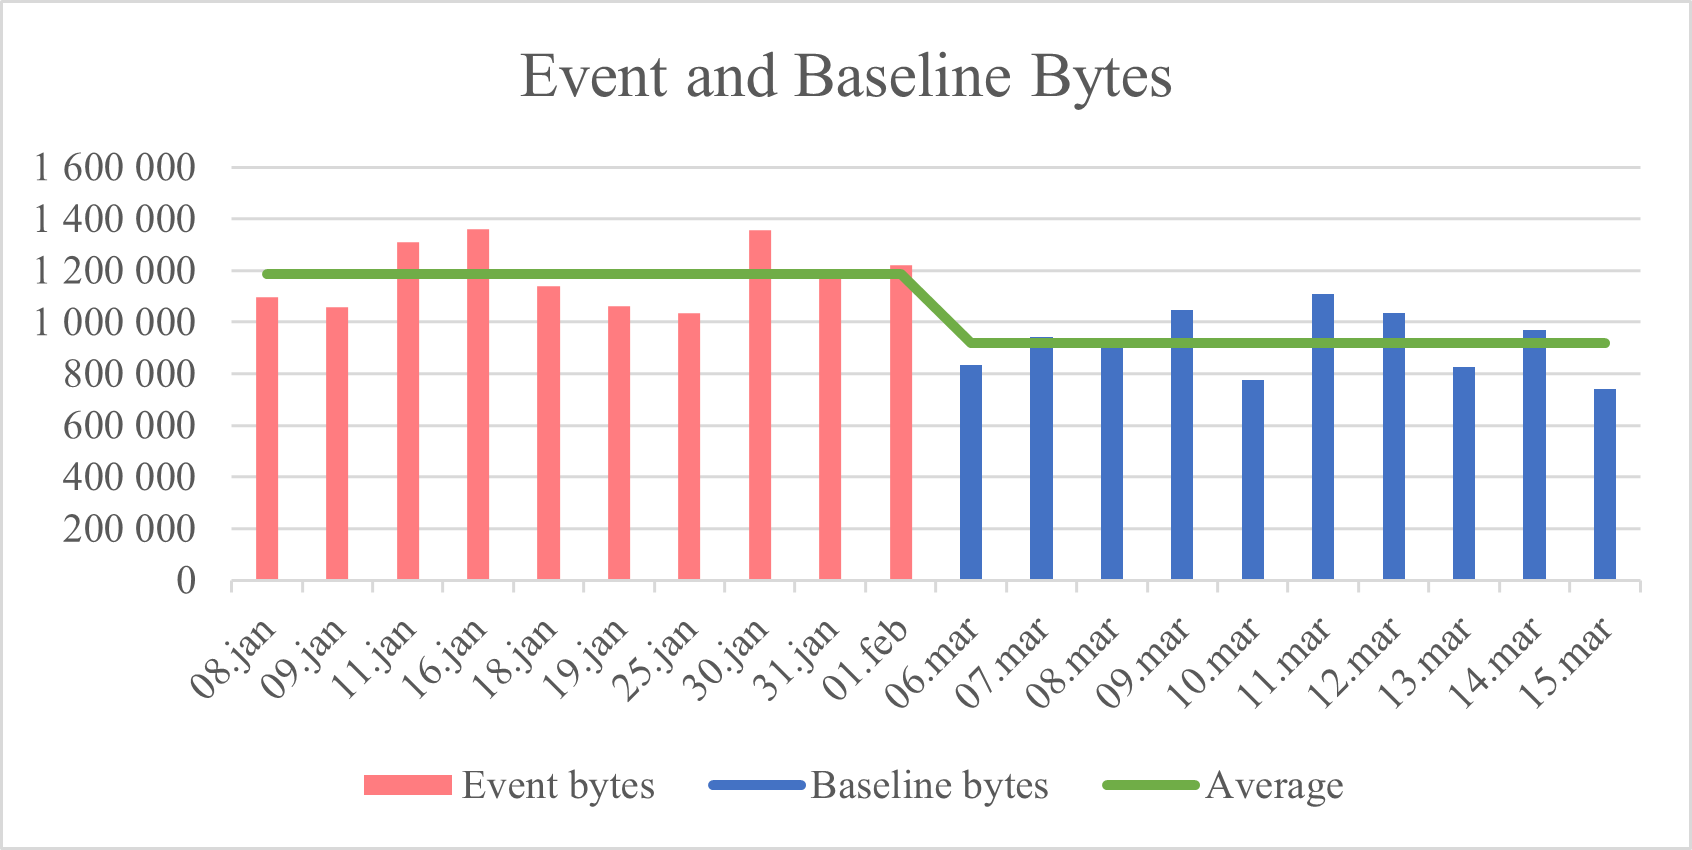
\includegraphics[width=1\hsize]{figures/Mill_Cooking_Calculations_Bytes.png} 
    \end{subfigure}
    \begin{subfigure}{0.8\textwidth}
        \centering
        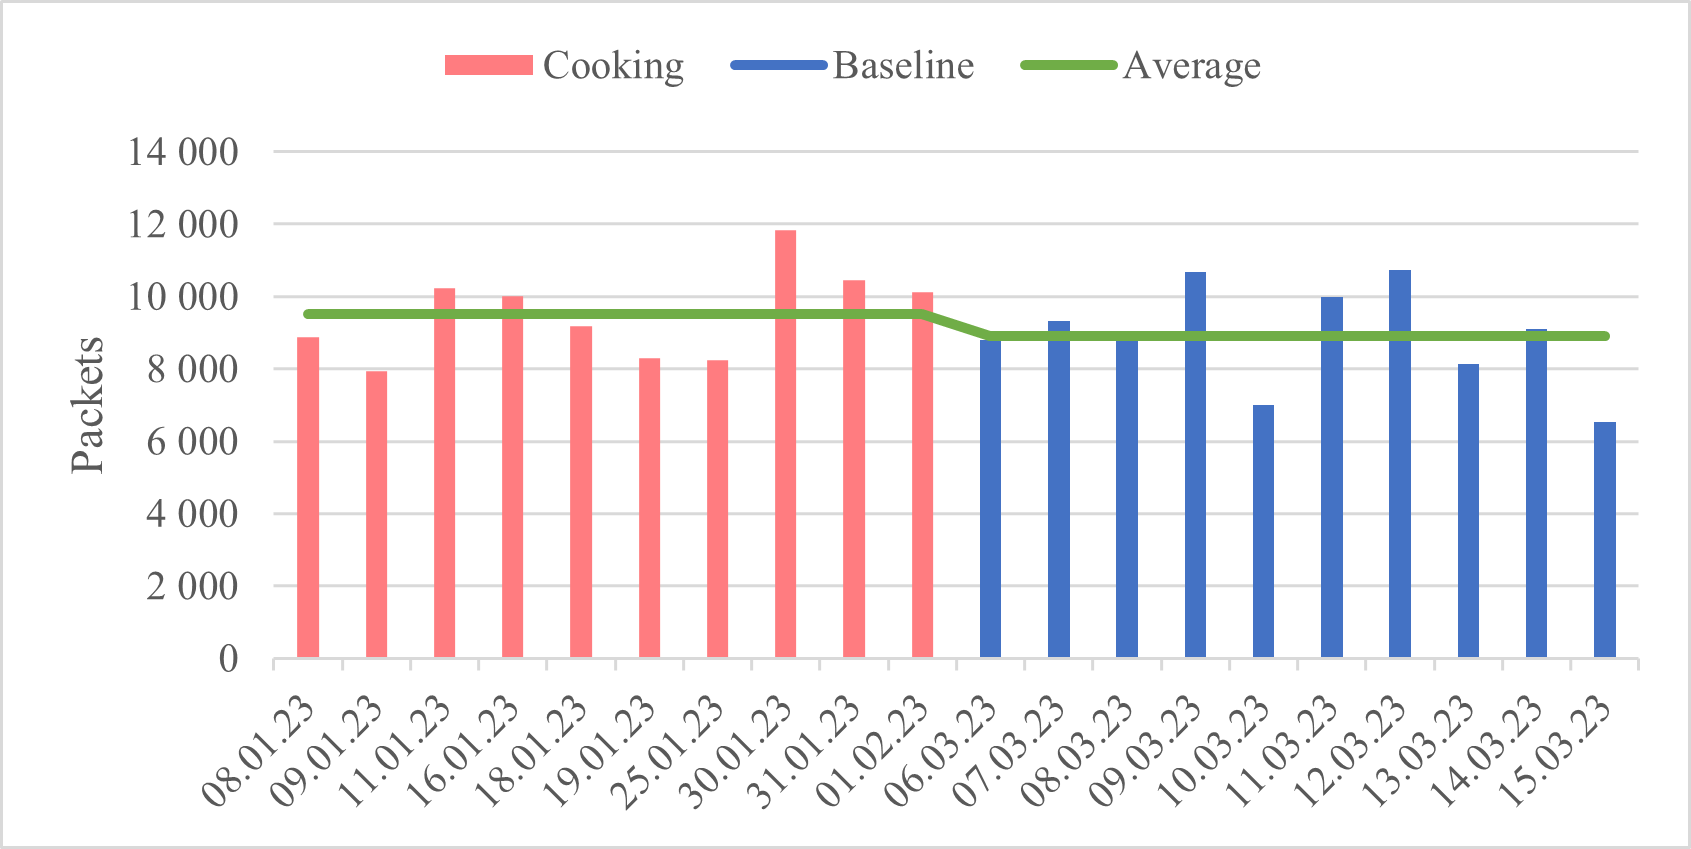
\includegraphics[width=1\hsize]{figures/Mill_Cooking_Calculations_Packets.png} 
    \end{subfigure}
    \caption{Mill: Graphical presentation of event and baseline cooking calculations with packets and bytes, including average value extracted from Table \ref{tab:NetatmoCookingCalculations}}
    \label{fig:MillCookingCalculations}
\end{figure}

The traffic pattern of the events and baseline are presented in Figure \ref{fig:MillCookingPackets1} and \ref{fig:MillCookingPackets2} for packets and in Figure \ref{fig:MillCookingBytes1} and \ref{fig:MillCookingBytes2} for bytes. In these figures, all graphs have the same minimum and maximum values on the y- and x-axis to be comparable. The graphs created from the different events are placed on the left side of the figure and framed in red, while the baseline is placed on the right side of the figure and framed in blue. The event times for when the event was ongoing are marked in red on the event graphs. Every graph within the same figure have the same minimum and maximum value on the x- and y-axis. 

\begin{figure}[H]
    \begin{subfigure}[b]{0.47\textwidth}
        \centering
        \tcbincludegraphics[size=fbox,width=1.1\hsize,colframe=red]{figures/Mill_Cooking_Packets_08.01.png}
    \end{subfigure}
    \begin{subfigure}[b]{0.47\textwidth}
        \centering
        \tcbincludegraphics[size=fbox,width=1.1\hsize, colframe=blue]{figures/Mill_Cooking_Baseline_Packets_06.03.png}
    \end{subfigure}
    \begin{subfigure}[b]{0.47\textwidth}
        \centering
        \tcbincludegraphics[size=fbox,width=1.1\hsize,colframe=red]{figures/Mill_Cooking_Packets_09.01.png}
    \end{subfigure}
    \begin{subfigure}[b]{0.47\textwidth}
        \centering
        \tcbincludegraphics[size=fbox,width=1.1\hsize,colframe=blue]{figures/Mill_Cooking_Baseline_Packets_07.03.png}
    \end{subfigure}
    \begin{subfigure}[b]{0.47\textwidth}
        \centering
        \tcbincludegraphics[size=fbox,width=1.1\hsize,colframe=red]{figures/Mill_Cooking_Packets_11.01.png}
    \end{subfigure}
    \begin{subfigure}[b]{0.47\textwidth}
        \centering
        \tcbincludegraphics[size=fbox,width=1.1\hsize,colframe=blue]{figures/Mill_Cooking_Baseline_Packets_08.03.png}
    \end{subfigure}
    \begin{subfigure}[b]{0.47\textwidth}
        \centering
        \tcbincludegraphics[size=fbox,width=1.1\hsize,colframe=red]{figures/Mill_Cooking_Packets_16.01.png}
    \end{subfigure}
    \begin{subfigure}[b]{0.47\textwidth}
        \centering
        \tcbincludegraphics[size=fbox,width=1.1\hsize,colframe=blue]{figures/Mill_Cooking_Baseline_Packets_09.03.png}
    \end{subfigure}
    \begin{subfigure}[b]{0.47\textwidth}
        \centering
        \tcbincludegraphics[size=fbox,width=1.1\hsize,colframe=red]{figures/Mill_Cooking_Packets_18.01.png}
    \end{subfigure}
    \begin{subfigure}[b]{0.47\textwidth}
        \centering
        \tcbincludegraphics[size=fbox,width=1.1\hsize,colframe=blue]{figures/Mill_Cooking_Baseline_Packets_10.03.png}
    \end{subfigure}
        \begin{subfigure}[b]{0.47\textwidth}
        \centering
        \tcbincludegraphics[size=fbox,width=1.1\hsize,colframe=red]{figures/Mill_Cooking_Packets_19.01.png}
    \end{subfigure}
    \begin{subfigure}[b]{0.47\textwidth}
        \centering
        \tcbincludegraphics[size=fbox,width=1.1\hsize,colframe=blue]{figures/Mill_Cooking_Baseline_Packets_11.03.png}
    \end{subfigure}
    \begin{subfigure}[b]{0.47\textwidth}
        \centering
        \tcbincludegraphics[size=fbox,width=1.1\hsize,colframe=red]{figures/Mill_Cooking_Packets_25.01.png}
    \end{subfigure}
    \hspace{0.6cm}
    \begin{subfigure}[b]{0.47\textwidth}
    \centering
        \tcbincludegraphics[size=fbox,width=1.1\hsize,colframe=blue]{figures/Mill_Cooking_Baseline_Packets_12.03.png}
        \end{subfigure}
    \caption{Mill: Graphs of traffic flows from the cooking events measured in packets with event graphs framed in red and baseline graphs framed in blue, Event times are marked in red on the event graphs.}
    \label{fig:MillCookingPackets1}
\end{figure}

\begin{figure}[H]
    \begin{subfigure}[b]{0.45\textwidth}
        \centering
        \tcbincludegraphics[size=fbox,width=1.1\hsize,colframe=red]{figures/Mill_Cooking_Packets_30.01.png}
    \end{subfigure}
    \begin{subfigure}[b]{0.45\textwidth}
        \centering
        \tcbincludegraphics[size=fbox,width=1.1\hsize, colframe=blue]{figures/Mill_Cooking_Baseline_Packets_13.03.png}
    \end{subfigure}
    \begin{subfigure}[b]{0.45\textwidth}
        \centering
        \tcbincludegraphics[size=fbox,width=1.1\hsize,colframe=red]{figures/Mill_Cooking_Packets_31.01.png}
    \end{subfigure}
    \begin{subfigure}[b]{0.45\textwidth}
        \centering
        \tcbincludegraphics[size=fbox,width=1.1\hsize,colframe=blue]{figures/Mill_Cooking_Baseline_Packets_14.03.png}
    \end{subfigure}
    \begin{subfigure}[b]{0.45\textwidth}
        \centering
        \tcbincludegraphics[size=fbox,width=1.1\hsize,colframe=red]{figures/Mill_Cooking_Packets_01.02.png}
    \end{subfigure}
    \hspace{1.1cm}
    \begin{subfigure}[b]{0.45\textwidth}
        \centering
        \tcbincludegraphics[size=fbox,width=1.1\hsize,colframe=blue]{figures/Mill_Cooking_Baseline_Packets_15.03.png}
    \end{subfigure}
    \caption{Mill: Continuing from Figure \ref{fig:MillCookingPackets1}}
    \label{fig:MillCookingPackets2}
\end{figure}

\begin{figure}[H]
    \begin{subfigure}[b]{0.45\textwidth}
        \centering
        \tcbincludegraphics[size=fbox,width=1.1\hsize,colframe=red]{figures/Mill_Cooking_Bytes_30.01.png}
    \end{subfigure}
    \begin{subfigure}[b]{0.45\textwidth}
        \centering
        \tcbincludegraphics[size=fbox,width=1.1\hsize, colframe=blue]{figures/Mill_Cooking_Baseline_Bytes_13.03.png}
    \end{subfigure}
    \begin{subfigure}[b]{0.45\textwidth}
        \centering
        \tcbincludegraphics[size=fbox,width=1.1\hsize,colframe=red]{figures/Mill_Cooking_Bytes_31.01.png}
    \end{subfigure}
    \begin{subfigure}[b]{0.45\textwidth}
        \centering
        \tcbincludegraphics[size=fbox,width=1.1\hsize,colframe=blue]{figures/Mill_Cooking_Baseline_Bytes_14.03.png}
    \end{subfigure}
    \begin{subfigure}[b]{0.45\textwidth}
        \centering
        \tcbincludegraphics[size=fbox,width=1.1\hsize,colframe=red]{figures/Mill_Cooking_Bytes_01.02.png}
    \end{subfigure}
    \hspace{1.1cm}
    \begin{subfigure}[b]{0.45\textwidth}
        \centering
        \tcbincludegraphics[size=fbox,width=1.1\hsize,colframe=blue]{figures/Mill_Cooking_Baseline_Bytes_15.03.png}
    \end{subfigure}
    \caption{Mill: Remaining graphs from Figure \ref{fig:NetatmoCookingBytes2}}
    \label{fig:MillCookingBytes1}
\end{figure}

\begin{figure}[H]
    \begin{subfigure}[b]{0.47\textwidth}
        \centering
        \tcbincludegraphics[size=fbox,width=1.1\hsize,colframe=red]{figures/Mill_Cooking_Bytes_08.01.png}
    \end{subfigure}
    \begin{subfigure}[b]{0.47\textwidth}
        \centering
        \tcbincludegraphics[size=fbox,width=1.1\hsize,colframe=blue]{figures/Mill_Cooking_Baseline_Bytes_06.03.png}
    \end{subfigure}
    \begin{subfigure}[b]{0.47\textwidth}
        \centering
        \tcbincludegraphics[size=fbox,width=1.1\hsize,colframe=red]{figures/Mill_Cooking_Bytes_09.01.png}
    \end{subfigure}
    \begin{subfigure}[b]{0.47\textwidth}
        \centering
        \tcbincludegraphics[size=fbox,width=1.1\hsize,colframe=blue]{figures/Mill_Cooking_Baseline_Bytes_07.03.png}
    \end{subfigure}
    \begin{subfigure}[b]{0.47\textwidth}
        \centering
        \tcbincludegraphics[size=fbox,width=1.1\hsize,colframe=red]{figures/Mill_Cooking_Bytes_11.01.png}
    \end{subfigure}
    \begin{subfigure}[b]{0.47\textwidth}
        \centering
        \tcbincludegraphics[size=fbox,width=1.1\hsize,colframe=blue]{figures/Mill_Cooking_Baseline_Bytes_08.03.png}
    \end{subfigure}
    \begin{subfigure}[b]{0.47\textwidth}
        \centering
        \tcbincludegraphics[size=fbox,width=1.1\hsize,colframe=red]{figures/Mill_Cooking_Bytes_16.01.png}
    \end{subfigure}
    \begin{subfigure}[b]{0.47\textwidth}
        \centering
        \tcbincludegraphics[size=fbox,width=1.1\hsize,colframe=blue]{figures/Mill_Cooking_Baseline_Bytes_09.03.png}
    \end{subfigure}
    \begin{subfigure}[b]{0.47\textwidth}
        \centering
        \tcbincludegraphics[size=fbox,width=1.1\hsize,colframe=red]{figures/Mill_Cooking_Bytes_18.01.png}
    \end{subfigure}
    \begin{subfigure}[b]{0.47\textwidth}
        \centering
        \tcbincludegraphics[size=fbox,width=1.1\hsize,colframe=blue]{figures/Mill_Cooking_Baseline_Bytes_10.03.png}
    \end{subfigure}
        \begin{subfigure}[b]{0.47\textwidth}
        \centering
        \tcbincludegraphics[size=fbox,width=1.1\hsize,colframe=red]{figures/Mill_Cooking_Bytes_19.01.png}
    \end{subfigure}
    \begin{subfigure}[b]{0.47\textwidth}
        \centering
        \tcbincludegraphics[size=fbox,width=1.1\hsize,colframe=blue]{figures/Mill_Cooking_Baseline_Bytes_11.03.png}
    \end{subfigure}
    \begin{subfigure}[b]{0.47\textwidth}
        \centering
        \tcbincludegraphics[size=fbox,width=1.1\hsize,colframe=red]{figures/Mill_Cooking_Bytes_25.01.png}
    \end{subfigure}
    \hspace{0.6cm}
    \begin{subfigure}[b]{0.47\textwidth}
    \centering
        \tcbincludegraphics[size=fbox,width=1.1\hsize,colframe=blue]{figures/Mill_Cooking_Baseline_Bytes_12.03.png}
        \end{subfigure}
    \caption{Mill: Graphs of traffic flows from the cooking events measured in bytes with event graphs framed in red and baseline graphs framed in blue, Event times are marked in red on the event graphs.} 
    \label{fig:MillCookingBytes2}
\end{figure}

Comparing Table \ref{tab:MillCookingCalculations} and \ref{tab:MillBaselineCookingCalculations} shows that the amount of packets sent to and from the device is around the same amount and not a significant difference between the two. The average values for packets in Table \ref{tab:MillComparingBaselineAndCookingCalculations} also shows that the values are similar to each other. For bytes, the calculations shows that when an event is ongoing, the overall values are higher than for standard baseline traffic. The comparison in Table \ref{tab:MillComparingBaselineAndCookingCalculations} shows that the average value for events are 266,308 bytes higher. The same is presented in Figure \ref{fig:MillCookingCalculations} where there are a bigger difference in bytes than packets for events and baseline traffic. For the biggest packet sent, the packet sizes varies from around 450 bytes to 1,550 bytes for events and baseline traffic over the same time, shown in Table \ref{tab:MillCookingCalculations} and \ref{tab:MillBaselineCookingCalculations}. 
\\\\
The graphs in Figure \ref{fig:MillCookingPackets1} and \ref{fig:MillCookingPackets2} for packets and Figure \ref{fig:MillCookingBytes1} and \ref{fig:MillCookingBytes2} for bytes does not show a significant change in traffic pattern from when an event is ongoing in the graphs framed in red and the standard traffic pattern from the baseline in the graphs framed in blue. The variations the calculations gave in bytes from the events and baseline is not very visible in the graphs as they both vary a lot. However, knowing that more bytes are sent during the events, it is possible to see that more of the event graphs have higher spikes than the baseline, but this is not applicable for all events. 

\newpage
\subsection{Nedis}
In Test Case 1: Cooking for Nedis, tables with numerical calculations are presented together with graphs of the traffic flow. In Table \ref{tab:NedisCookingCalculations} the total amount of packets and bytes including the biggest packet during the event are presented for each of the 10 cooking events. Table \ref{tab:NedisBaselineCookingCalculations} presents the same values, but in regards of the baseline pcaps. Table \ref{tab:NedisComparingBaselineAndCookingCalculations} compares the average values and standard deviation from the events and baseline for packets, bytes and biggest packet. Figure \ref{fig:NedisCookingCalculations} presents the calculations from Table \ref{tab:NedisCookingCalculations}, \ref{tab:NedisBaselineCookingCalculations} and \ref{tab:NedisComparingBaselineAndCookingCalculations} with packets and bytes together with the average value for both the event and baseline traffic to easier compare it.  

\begin{table}[H]
\centering
    \caption{Nedis event calculations for the cooking events}
\label{tab:NedisCookingCalculations}
    \begin{tabular}{|l|l|l|l|}
        \hline
        \textbf{Events}    & \textbf{Packets} & \textbf{Bytes}     & \textbf{Biggest packet} \\ \hline
        08.jan             & 24,494           & 3,318,519          & 485 bytes               \\ \hline
        09.jan             & 26,787           & 3,870,361          & 424 bytes               \\ \hline
        11.jan             & 24,381           & 3,550,947          & 424 bytes               \\ \hline
        16.jan             & 26,035           & 3,895,071          & 485 bytes               \\ \hline
        18.jan             & 25,398           & 3,233,845          & 424 bytes               \\ \hline
        19.jan             & 20,857           & 3,242,594          & 424 bytes               \\ \hline
        25.jan             & 24,233           & 3,095,693          & 424 bytes               \\ \hline
        30.jan             & 24,867           & 3,257,812          & 424 bytes               \\ \hline
        31.jan             & 23,882           & 3,179,117          & 424 bytes               \\ \hline
        01.feb             & 25,397           & 3,477,014          & 424 bytes               \\ \hline
    \end{tabular}
\end{table}

\begin{table}[H]
    \centering
    \caption{Nedis baseline calculations for the corresponding cooking event times}
    \begin{tabular}{|l|l|l|l|l|l|}
    \hline
        \textbf{Baseline} & \textbf{Packets} & \textbf{Bytes} & \textbf{Biggest packet} \\ \hline
        06.mar & 13,014 & 1,413,457 & 421 bytes \\ \hline
        07.mar & 18,634 & 2,001,978 & 421 bytes \\ \hline
        08.mar & 18,643 & 2,019,872 & 421 bytes \\ \hline
        09.mar & 21,885 & 2,606,363 & 424 bytes \\ \hline
        10.mar & 17,956 & 2,326,898 & 424 bytes \\ \hline
        11.mar & 18,380 & 2,126,816 & 485 bytes \\ \hline
        12.mar & 10,728 & 1,312,915 & 421 bytes \\ \hline
        13.mar & 15,815 & 1,968,872 & 424 bytes \\ \hline
        14.mar & 15,926 & 1,878,449 & 341 bytes \\ \hline
        15.mar & 19,260 & 2,524,793 & 458 bytes \\ \hline
    \end{tabular}
    \label{tab:NedisBaselineCookingCalculations}
\end{table}

\begin{table}[H]
    \centering
    \caption{Nedis: Comparing event and baseline calculations for the cooking test}
    \begin{tabular}{c|l|l|l|l|}
        \cline{2-5}
        \multicolumn{1}{l|}{}                                              & \textbf{Type} & \textbf{Packets} & \textbf{Bytes} & \textbf{Biggest packet} \\ \hline
        \multicolumn{1}{|c|}{\multirow{2}{*}{\textbf{Average}}}            & Event         & 24,633             & 3,412,097       & 436 bytes               \\ \cline{2-5} 
        \multicolumn{1}{|c|}{}                                             & Baseline      & 17,024             & 2,018,041       & 424 bytes                \\ \hline
        \multicolumn{1}{|c|}{\multirow{2}{*}{\textbf{Standard deviation}}} & Event         & 1,595              & 281,705         & 26 bytes                 \\ \cline{2-5} 
        \multicolumn{1}{|c|}{}                                             & Baseline      & 3,248              & 420,982         & 36 bytes               \\ \hline          
    \end{tabular}
    \label{tab:NedisComparingBaselineAndCookingCalculations}
\end{table}

\begin{figure}[H]
    \centering
    \begin{subfigure}{0.8\textwidth}
        \centering
        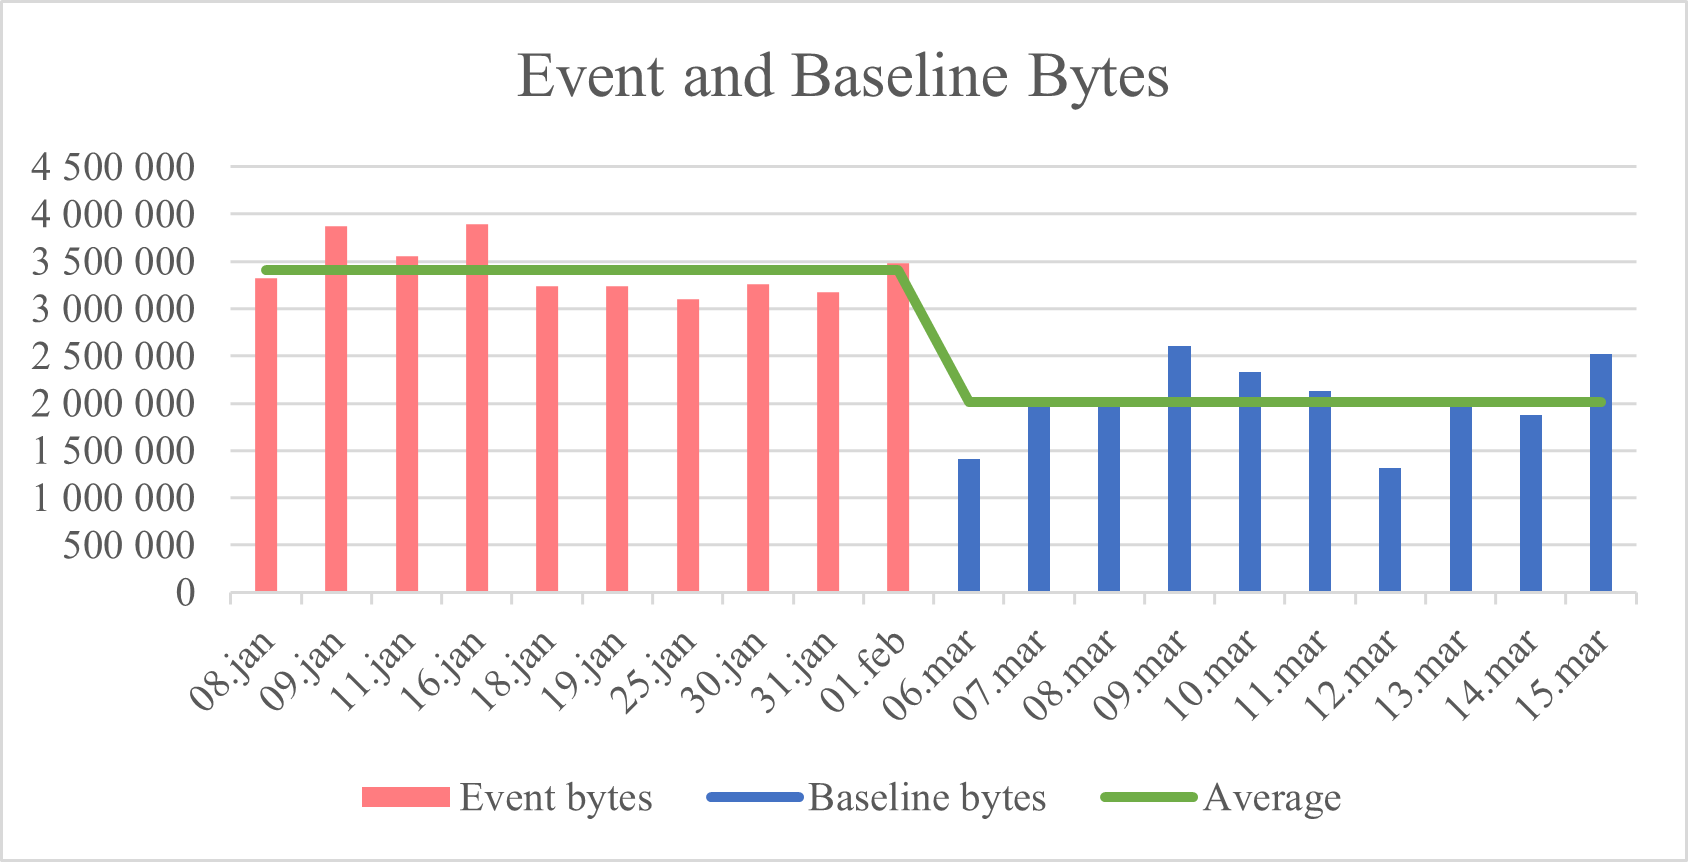
\includegraphics[width=1\hsize]{figures/Nedis_Cooking_Calculations_Bytes.png} 
    \end{subfigure}
    \begin{subfigure}{0.8\textwidth}
        \centering
        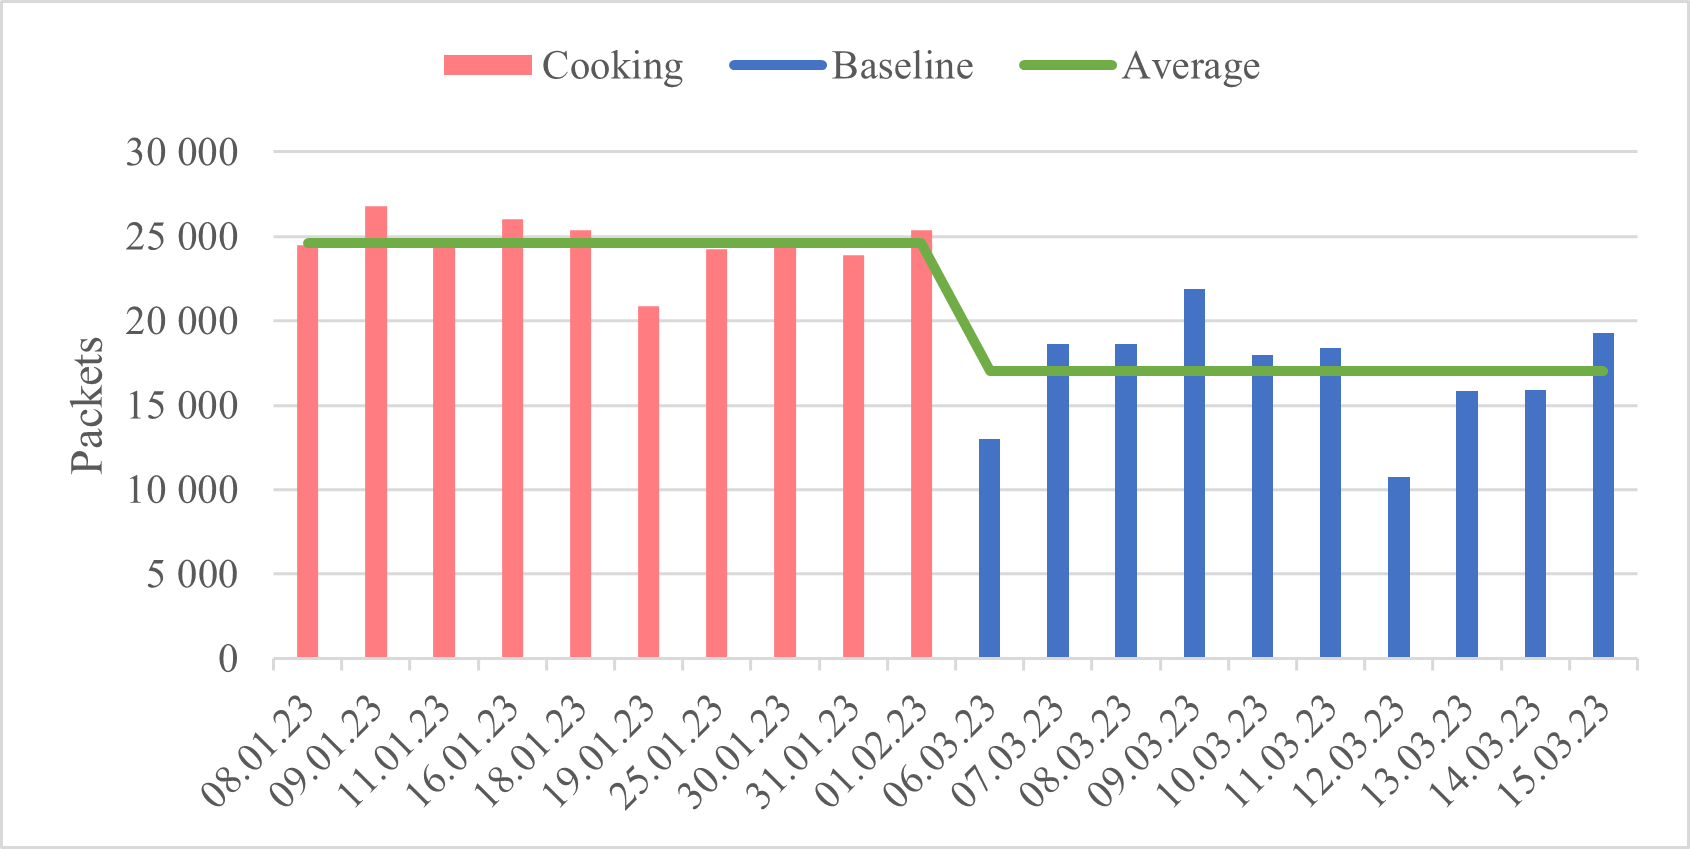
\includegraphics[width=1\hsize]{figures/Nedis_Cooking_Calculations_Packets.png} 
    \end{subfigure}
    \caption{Nedis: Graphical presentation of event and baseline cooking calculations with packets and bytes, including average value extracted from Table \ref{tab:NetatmoCookingCalculations}}
    \label{fig:NedisCookingCalculations}
\end{figure}

The graphical presentation of the traffic patterns during event are presented in Figure \ref{fig:NedisCookingPackets1} and \ref{fig:NedisCookingPackets2} for packets and in Figure \ref{fig:NedisCookingBytes1} and \ref{fig:NedisCookingBytes2} for bytes. In these figures, the corresponding graphs from the baseline traffic is also included to look for traffic changes during the events. In these figures, the graphs for events are placed on the left side of the figure and framed in red, while the baseline graphs are placed on the right side and framed in blue. The event graphs are marked with red when the event was ongoing. The minimum and maximum values on the x- and y-axis are equal for all graphs within the same figure. 

\begin{figure}[H]
    \begin{subfigure}[b]{0.47\textwidth}
        \centering
        \tcbincludegraphics[size=fbox,width=1.1\hsize,colframe=red]{figures/Nedis_Cooking_Packets_08.01.png}
    \end{subfigure}
    \begin{subfigure}[b]{0.47\textwidth}
        \centering
        \tcbincludegraphics[size=fbox,width=1.1\hsize, colframe=blue]{figures/Nedis_Cooking_Baseline_Packets_06.03.png}
    \end{subfigure}
    \begin{subfigure}[b]{0.47\textwidth}
        \centering
        \tcbincludegraphics[size=fbox,width=1.1\hsize,colframe=red]{figures/Nedis_Cooking_Packets_09.01.png}
    \end{subfigure}
    \begin{subfigure}[b]{0.47\textwidth}
        \centering
        \tcbincludegraphics[size=fbox,width=1.1\hsize,colframe=blue]{figures/Nedis_Cooking_Baseline_Packets_07.03.png}
    \end{subfigure}
    \begin{subfigure}[b]{0.47\textwidth}
        \centering
        \tcbincludegraphics[size=fbox,width=1.1\hsize,colframe=red]{figures/Nedis_Cooking_Packets_11.01.png}
    \end{subfigure}
    \begin{subfigure}[b]{0.47\textwidth}
        \centering
        \tcbincludegraphics[size=fbox,width=1.1\hsize,colframe=blue]{figures/Nedis_Cooking_Baseline_Packets_08.03.png}
    \end{subfigure}
    \begin{subfigure}[b]{0.47\textwidth}
        \centering
        \tcbincludegraphics[size=fbox,width=1.1\hsize,colframe=red]{figures/Nedis_Cooking_Packets_16.01.png}
    \end{subfigure}
    \begin{subfigure}[b]{0.47\textwidth}
        \centering
        \tcbincludegraphics[size=fbox,width=1.1\hsize,colframe=blue]{figures/Nedis_Cooking_Baseline_Packets_09.03.png}
    \end{subfigure}
    \begin{subfigure}[b]{0.47\textwidth}
        \centering
        \tcbincludegraphics[size=fbox,width=1.1\hsize,colframe=red]{figures/Nedis_Cooking_Packets_18.01.png}
    \end{subfigure}
    \begin{subfigure}[b]{0.47\textwidth}
        \centering
        \tcbincludegraphics[size=fbox,width=1.1\hsize,colframe=blue]{figures/Nedis_Cooking_Baseline_Packets_10.03.png}
    \end{subfigure}
        \begin{subfigure}[b]{0.47\textwidth}
        \centering
        \tcbincludegraphics[size=fbox,width=1.1\hsize,colframe=red]{figures/Nedis_Cooking_Packets_19.01.png}
    \end{subfigure}
    \begin{subfigure}[b]{0.47\textwidth}
        \centering
        \tcbincludegraphics[size=fbox,width=1.1\hsize,colframe=blue]{figures/Nedis_Cooking_Baseline_Packets_11.03.png}
    \end{subfigure}
    \begin{subfigure}[b]{0.47\textwidth}
        \centering
        \tcbincludegraphics[size=fbox,width=1.1\hsize,colframe=red]{figures/Nedis_Cooking_Packets_25.01.png}
    \end{subfigure}
    \hspace{0.6cm}
    \begin{subfigure}[b]{0.47\textwidth}
    \centering
        \tcbincludegraphics[size=fbox,width=1.1\hsize,colframe=blue]{figures/Nedis_Cooking_Baseline_Packets_12.03.png}
        \end{subfigure}
    \caption{Nedis: Graphs of traffic flows from the cooking events measured in packets with event graphs framed in red and baseline graphs framed in blue, Event times are marked in red on the event graphs.}
    \label{fig:NedisCookingPackets1}
\end{figure}

\begin{figure}[H]
    \begin{subfigure}[b]{0.45\textwidth}
        \centering
        \tcbincludegraphics[size=fbox,width=1.1\hsize,colframe=red]{figures/Nedis_Cooking_Packets_30.01.png}
    \end{subfigure}
    \begin{subfigure}[b]{0.45\textwidth}
        \centering
        \tcbincludegraphics[size=fbox,width=1.1\hsize, colframe=blue]{figures/Nedis_Cooking_Baseline_Packets_13.03.png}
    \end{subfigure}
    \begin{subfigure}[b]{0.45\textwidth}
        \centering
        \tcbincludegraphics[size=fbox,width=1.1\hsize,colframe=red]{figures/Nedis_Cooking_Packets_31.01.png}
    \end{subfigure}
    \begin{subfigure}[b]{0.45\textwidth}
        \centering
        \tcbincludegraphics[size=fbox,width=1.1\hsize,colframe=blue]{figures/Nedis_Cooking_Baseline_Packets_14.03.png}
    \end{subfigure}
    \begin{subfigure}[b]{0.45\textwidth}
        \centering
        \tcbincludegraphics[size=fbox,width=1.1\hsize,colframe=red]{figures/Nedis_Cooking_Packets_01.02.png}
    \end{subfigure}
    \hspace{1.1cm}
    \begin{subfigure}[b]{0.45\textwidth}
        \centering
        \tcbincludegraphics[size=fbox,width=1.1\hsize,colframe=blue]{figures/Nedis_Cooking_Baseline_Packets_15.03.png}
    \end{subfigure}
    \caption{Nedis: First from Figure \ref{fig:NedisCookingPackets1}}
    \label{fig:NedisCookingPackets2}
\end{figure}

\begin{figure}[H]
    \begin{subfigure}[b]{0.45\textwidth}
        \centering
        \tcbincludegraphics[size=fbox,width=1.1\hsize,colframe=red]{figures/Nedis_Cooking_Bytes_30.01.png}
    \end{subfigure}
    \begin{subfigure}[b]{0.45\textwidth}
        \centering
        \tcbincludegraphics[size=fbox,width=1.1\hsize, colframe=blue]{figures/Nedis_Cooking_Baseline_Bytes_13.03.png}
    \end{subfigure}
    \begin{subfigure}[b]{0.45\textwidth}
        \centering
        \tcbincludegraphics[size=fbox,width=1.1\hsize,colframe=red]{figures/Nedis_Cooking_Bytes_31.01.png}
    \end{subfigure}
    \begin{subfigure}[b]{0.45\textwidth}
        \centering
        \tcbincludegraphics[size=fbox,width=1.1\hsize,colframe=blue]{figures/Nedis_Cooking_Baseline_Bytes_14.03.png}
    \end{subfigure}
    \begin{subfigure}[b]{0.45\textwidth}
        \centering
        \tcbincludegraphics[size=fbox,width=1.1\hsize,colframe=red]{figures/Nedis_Cooking_Bytes_01.02.png}
    \end{subfigure}
    \hspace{1.1cm}
    \begin{subfigure}[b]{0.45\textwidth}
        \centering
        \tcbincludegraphics[size=fbox,width=1.1\hsize,colframe=blue]{figures/Nedis_Cooking_Baseline_Bytes_15.03.png}
    \end{subfigure}
    \caption{Nedis: Remaining graphs from Figure \ref{fig:NedisCookingBytes2}}
    \label{fig:NedisCookingBytes1}
\end{figure}

\begin{figure}[H]
    \begin{subfigure}[b]{0.47\textwidth}
        \centering
        \tcbincludegraphics[size=fbox,width=1.1\hsize,colframe=red]{figures/Nedis_Cooking_Bytes_08.01.png}
    \end{subfigure}
    \begin{subfigure}[b]{0.47\textwidth}
        \centering
        \tcbincludegraphics[size=fbox,width=1.1\hsize,colframe=blue]{figures/Nedis_Cooking_Baseline_Bytes_06.03.png}
    \end{subfigure}
    \begin{subfigure}[b]{0.47\textwidth}
        \centering
        \tcbincludegraphics[size=fbox,width=1.1\hsize,colframe=red]{figures/Nedis_Cooking_Bytes_09.01.png}
    \end{subfigure}
    \begin{subfigure}[b]{0.47\textwidth}
        \centering
        \tcbincludegraphics[size=fbox,width=1.1\hsize,colframe=blue]{figures/Nedis_Cooking_Baseline_Bytes_07.03.png}
    \end{subfigure}
    \begin{subfigure}[b]{0.47\textwidth}
        \centering
        \tcbincludegraphics[size=fbox,width=1.1\hsize,colframe=red]{figures/Nedis_Cooking_Bytes_11.01.png}
    \end{subfigure}
    \begin{subfigure}[b]{0.47\textwidth}
        \centering
        \tcbincludegraphics[size=fbox,width=1.1\hsize,colframe=blue]{figures/Nedis_Cooking_Baseline_Bytes_08.03.png}
    \end{subfigure}
    \begin{subfigure}[b]{0.47\textwidth}
        \centering
        \tcbincludegraphics[size=fbox,width=1.1\hsize,colframe=red]{figures/Nedis_Cooking_Bytes_16.01.png}
    \end{subfigure}
    \begin{subfigure}[b]{0.47\textwidth}
        \centering
        \tcbincludegraphics[size=fbox,width=1.1\hsize,colframe=blue]{figures/Nedis_Cooking_Baseline_Bytes_09.03.png}
    \end{subfigure}
    \begin{subfigure}[b]{0.47\textwidth}
        \centering
        \tcbincludegraphics[size=fbox,width=1.1\hsize,colframe=red]{figures/Nedis_Cooking_Bytes_18.01.png}
    \end{subfigure}
    \begin{subfigure}[b]{0.47\textwidth}
        \centering
        \tcbincludegraphics[size=fbox,width=1.1\hsize,colframe=blue]{figures/Nedis_Cooking_Baseline_Bytes_10.03.png}
    \end{subfigure}
        \begin{subfigure}[b]{0.47\textwidth}
        \centering
        \tcbincludegraphics[size=fbox,width=1.1\hsize,colframe=red]{figures/Nedis_Cooking_Bytes_19.01.png}
    \end{subfigure}
    \begin{subfigure}[b]{0.47\textwidth}
        \centering
        \tcbincludegraphics[size=fbox,width=1.1\hsize,colframe=blue]{figures/Nedis_Cooking_Baseline_Bytes_11.03.png}
    \end{subfigure}
    \begin{subfigure}[b]{0.47\textwidth}
        \centering
        \tcbincludegraphics[size=fbox,width=1.1\hsize,colframe=red]{figures/Nedis_Cooking_Bytes_25.01.png}
    \end{subfigure}
    \hspace{0.6cm}
    \begin{subfigure}[b]{0.47\textwidth}
    \centering
        \tcbincludegraphics[size=fbox,width=1.1\hsize,colframe=blue]{figures/Nedis_Cooking_Baseline_Bytes_12.03.png}
        \end{subfigure}
    \caption{Nedis: Graphs of traffic flows from the cooking events measured in bytes with event graphs framed in red and baseline graphs framed in blue, Event times are marked in red on the event graphs.} 
    \label{fig:NedisCookingBytes2}
\end{figure}

Comparing Table \ref{tab:NedisCookingCalculations} and \ref{tab:NedisBaselineCookingCalculations} shows overall that during the events, more packets and events are sent than during standard baseline traffic. While for the biggest packet during the cooking-time, there are not a significant difference to when an event is ongoing. The same is shown in Table \ref{tab:NedisComparingBaselineAndCookingCalculations} where the average for both packets and bytes are higher during events. This is also visible in Figure \ref{fig:NedisCookingCalculations} where all the blue marked bars are lower than the red marked graphs for events. 
\\\\
The graphs in Figure \ref{fig:NedisCookingPackets1} and \ref{fig:NedisCookingPackets2} gives the same results, that overall during an event the traffic pattern is different then for the baseline. For Figure \ref{fig:NedisCookingBytes1} and \ref{fig:NedisCookingBytes2} the difference is much clearer than for packets. The graphs for baseline are significantly lower in bytes sent and received to the device than when the event is ongoing. 

\newpage
\section{Test Case 2: Showering}
This chapter presents the results and analysis conducted on Test Case 2: Showering. The first sub-section describes the general evaluation which is applicable for all the devices and the next three sub-sections presents the results and analysis for each of the devices separately. 
\subsection{General}
The showering event has been conducted 10 times and Table \ref{tab:ShoweringDates} presents the 10 different dates and exact times for when the event was ongoing.
\begin{table}[H]
    \centering
    \caption{Date and time for Test Case 2: Showering events}
    \begin{adjustbox}{width=1\textwidth} 
        \begin{tabular}{l|l|l|l|l|l|l|l|l|l|l|}
            \cline{2-11}
                & 08.01 & 09.01 & 11.01 & 16.01 & 18.01 & 19.01 & 25.01 & 30.01 & 31.01 & 01.02 \\ \hline
            \multicolumn{1}{|l|}{Started event}  & 19:59 & 20:14 & 20:01 & 20:12 & 20:02 & 20:00 & 20:03 & 20:00 & 20:01 & 20:00 \\ \hline
            \multicolumn{1}{|l|}{Finished event} & 20:14 & 20:34 & 20:17 & 20:31 & 20:19 & 20:16 & 20:19 & 20:18 & 20:17 & 20:16 \\ \hline
        \end{tabular}
    \end{adjustbox}
    \label{tab:ShoweringDates}
\end{table}

To be able to compare the events to each other and the standard baseline traffic, all the pcaps created for this event will have the same start and finish time. Graphically, each event will have marked at what time the actual event was ongoing to separate from before and after the event. When deciding which start and end time for these events, the earliest start and latest finish are used. These times are then added 30 minutes before and after to cover at least 30 minutes before and after each event. This gives the following values to use for further analysis:

\begin{itemize}
    \item Earliest Event Start: 19:59
    \item Latest Event Finished: 20:34
    \item Packet Capture Files Start: 19:29
    \item Packet Capture Files End: 21:04
\end{itemize}

These times results in the following filters added to create the pcaps for each event:
\begin{itemize}
    \item frame.time >= "Month Date, Year 19:29:00" \&\& frame.time <= "Month Date, Year 21:04:00"
\end{itemize}

\newpage
\subsection{Netatmo}
For Netatmo, the 10 event packet captures for the showering event are presented both graphically in figures and numerically in tables. Table \ref{tab:NetatmoShowerCalculations} shows packets, bytes and the biggest packet in each of the packet captures. Table \ref{tab:NetatmoBaselineShowerCalculations} presents the same calculations, but for the corresponding baseline pcaps. In Table \ref{tab:NetatmoComparingBaselineAndShowerCalculations}, the average and standard deviation values from Table \ref{tab:NetatmoShowerCalculations} and \ref{tab:NetatmoBaselineShowerCalculations} are compared to each other. In context of these three tables, two graphical presentations of total bytes and packets including the average values for events and baseline are presented to compare events to the baseline traffic in Figure \ref{fig:NetatmoShowerCalculations}. 

\begin{table}[H]
    \centering
    \caption{Netatmo event calculations for the showering events}
    \begin{tabular}{|l|l|l|l|l|l|}
    \hline
        \textbf{Event dates} & \textbf{Packets} & \textbf{Bytes} & \textbf{Biggest packet} \\ \hline
        08.jan & 870   & 118,119 & 407 bytes\\ \hline
        09.jan & 816   & 112,821 & 407 bytes \\ \hline
        11.jan & 1,075 & 145,838 & 407 bytes\\ \hline
        16.jan & 667   & 90,370  & 407 bytes\\ \hline
        18.jan & 802   & 109,285 & 407 bytes\\ \hline
        19.jan & 636   & 85,860  & 407 bytes \\ \hline
        25.jan & 897   & 120,580 & 134 bytes \\ \hline
        30.jan & 862   & 116,726 & 134 bytes \\ \hline
        31.jan & 704   & 94,140  & 136 bytes \\ \hline
        01.feb & 694   & 94,053  & 407 bytes \\ \hline
    \end{tabular}
    \label{tab:NetatmoShowerCalculations}
\end{table}

\begin{table}[H]
    \centering
    \caption{Netatmo baseline calculations for the corresponding showering event times}
    \begin{tabular}{|l|l|l|l|}
    \hline
        \textbf{Baseline} & \textbf{Packets} & \textbf{Bytes} & \textbf{Biggest packet} \\ \hline
        06.mar & 614 & 81,600  & 136 bytes\\ \hline
        07.mar & 710 & 94,869  & 407 bytes\\ \hline
        08.mar & 780 & 94,892  & 160 bytes \\ \hline
        09.mar & 884 & 118,116 & 134 bytes \\ \hline
        10.mar & 594 & 79,258  & 136 bytes \\ \hline
        11.mar & 615 & 82,664  & 407 bytes \\ \hline
        12.mar & 857 & 116,703 & 407 bytes \\ \hline
        13.mar & 514 & 68,470  & 136 bytes \\ \hline
        14.mar & 808 & 108,120 & 407 bytes \\ \hline
        15.mar & 731 & 97,682  & 134 bytes \\ \hline
    \end{tabular}
    \label{tab:NetatmoBaselineShowerCalculations}
\end{table}

\begin{table}[H]
    \centering
    \caption{Netatmo: Comparing event and baseline calculations for the showering test}
    \begin{tabular}{c|l|l|l|l|}
        \cline{2-5}
        \multicolumn{1}{l|}{}                                              & \textbf{Type} & \textbf{Packets} & \textbf{Bytes} & \textbf{Biggest packet} \\ \hline
        \multicolumn{1}{|c|}{\multirow{2}{*}{\textbf{Average}}}            & Event         & 802              & 108,779        & 325 bytes               \\ \cline{2-5} 
        \multicolumn{1}{|c|}{}                                             & Baseline      & 711              & 94,237         & 246 bytes                \\ \hline
        \multicolumn{1}{|c|}{\multirow{2}{*}{\textbf{Standard deviation}}} & Event         & 133              & 18,181         & 132 bytes                 \\ \cline{2-5} 
        \multicolumn{1}{|c|}{}                                             & Baseline      & 123              & 16,541         & 138 bytes               \\ \hline          
    \end{tabular}
    \label{tab:NetatmoComparingBaselineAndShowerCalculations}
\end{table}

\begin{figure}[H]
    \centering
    \begin{subfigure}{0.8\textwidth}
       \centering
       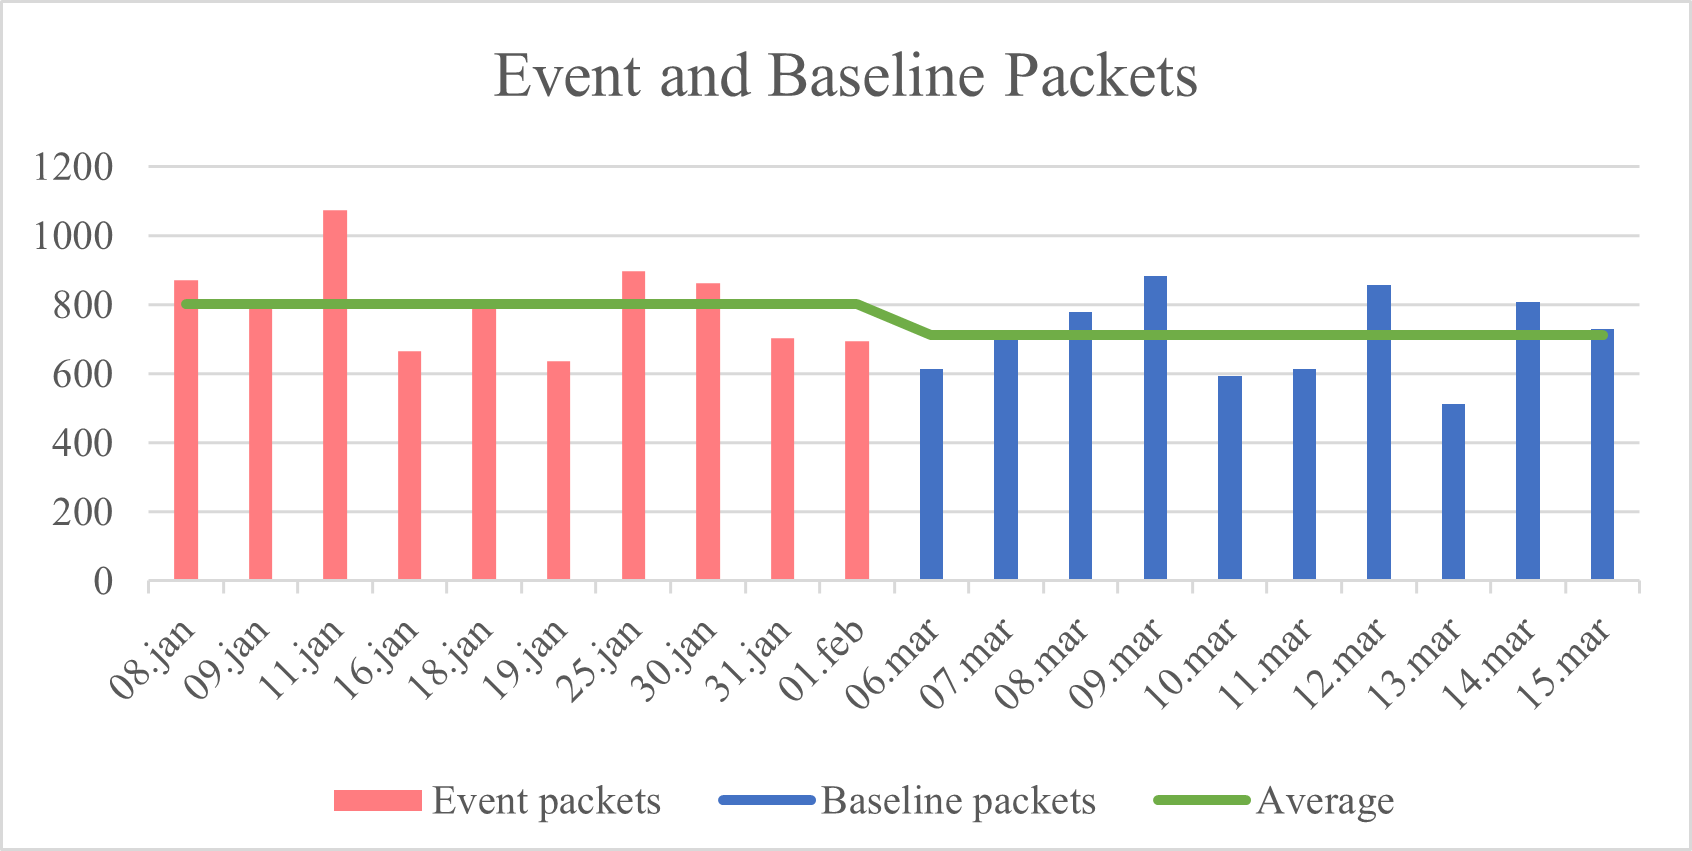
\includegraphics[width=1\hsize]{figures/Netatmo_Shower_Calculations_Packets.png} 
    \end{subfigure}
    \begin{subfigure}{0.8\textwidth}
        \centering
        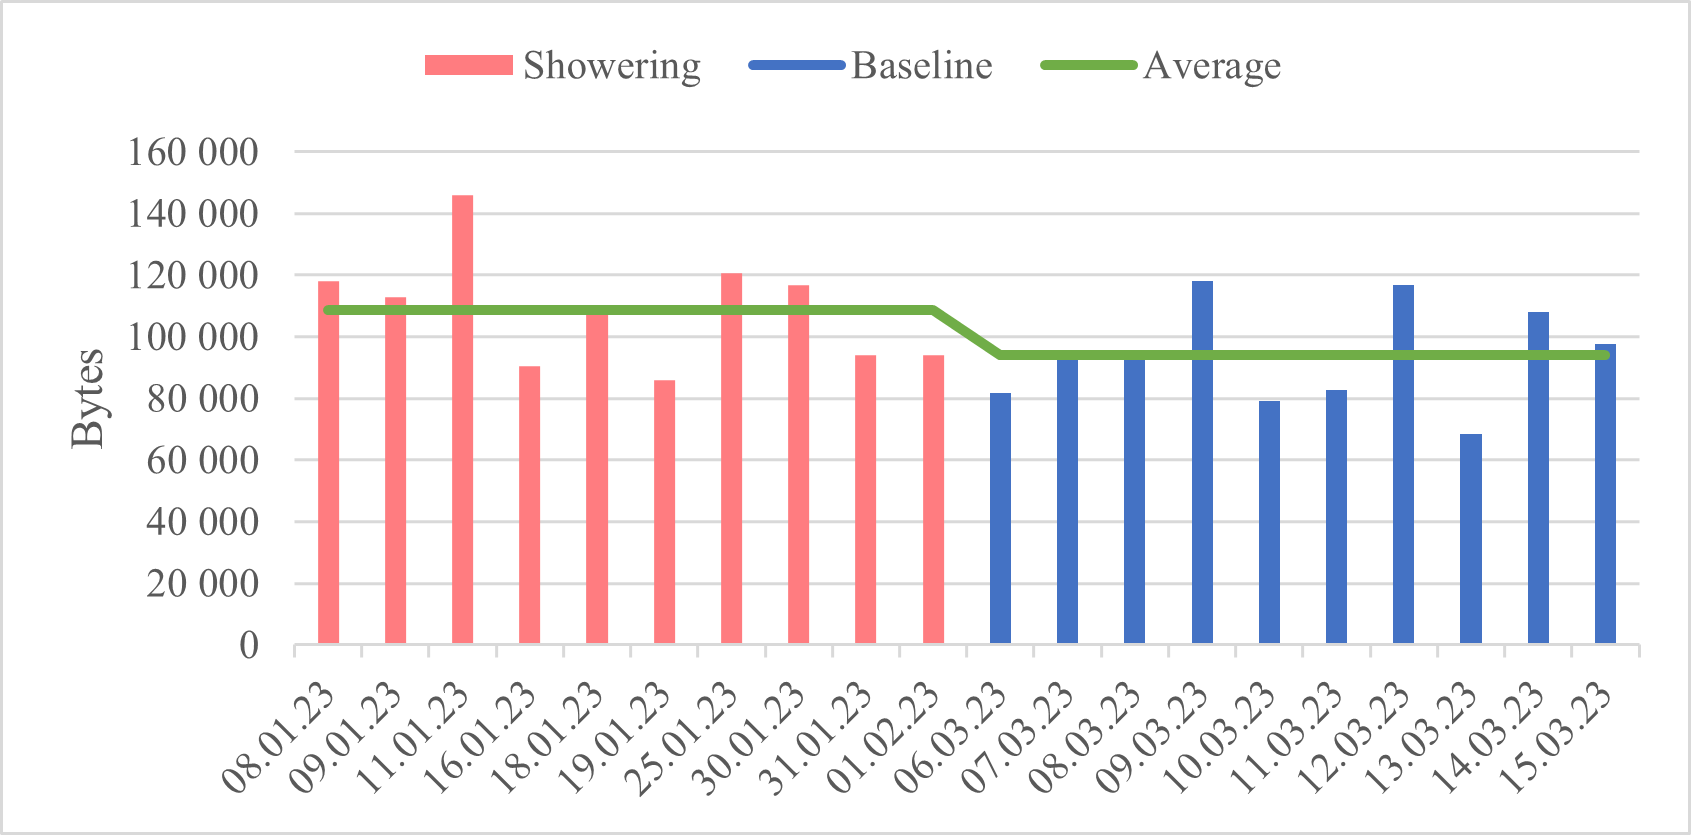
\includegraphics[width=1\hsize]{figures/Netatmo_Shower_Calculations_Bytes.png} 
    \end{subfigure}
    \caption{Netatmo: Graphical presentation of event and baseline showering calculations with packets and bytes, including average value extracted from Table \ref{tab:NetatmoCookingCalculations}}
    \label{fig:NetatmoShowerCalculations}
\end{figure}

Figure \ref{fig:NetatmoShowerPackets1} and \ref{fig:NetatmoShowerPackets2} gives the graphical presentation of the traffic flow during the showering times with the total number of packets sent and received on the y-axis. Figure \ref{fig:NetatmoShowerBytes1} and \ref{fig:NetatmoShowerBytes2} shows the same, but with bytes on the y-axis. The figures over the traffic flow all have the same minimum and maximum values on the y- and x-axis and event graphs are placed on the left side of the figure with a red frame, while baseline graphs are placed on the right side of the figure with a blue frame. The events are marked with a red area on the event graphs to look for changes in traffic pattern at that specific time. The minimum and maximum values on the x- and y-axis are equal for all the graphs within the same figure. 

\begin{figure}[H]
    \begin{subfigure}[b]{0.47\textwidth}
        \centering
        \tcbincludegraphics[size=fbox,width=1.1\hsize,colframe=red]{figures/Netatmo_Shower_Packets_08.01.png}
    \end{subfigure}
    \begin{subfigure}[b]{0.47\textwidth}
        \centering
        \tcbincludegraphics[size=fbox,width=1.1\hsize, colframe=blue]{figures/Netatmo_Shower_Baseline_Packets_06.03.png}
    \end{subfigure}
    \begin{subfigure}[b]{0.47\textwidth}
        \centering
        \tcbincludegraphics[size=fbox,width=1.1\hsize,colframe=red]{figures/Netatmo_Shower_Packets_09.01.png}
    \end{subfigure}
    \begin{subfigure}[b]{0.47\textwidth}
        \centering
        \tcbincludegraphics[size=fbox,width=1.1\hsize,colframe=blue]{figures/Netatmo_Shower_Baseline_Packets_07.03.png}
    \end{subfigure}
    \begin{subfigure}[b]{0.47\textwidth}
        \centering
        \tcbincludegraphics[size=fbox,width=1.1\hsize,colframe=red]{figures/Netatmo_Shower_Packets_11.01.png}
    \end{subfigure}
    \begin{subfigure}[b]{0.47\textwidth}
        \centering
        \tcbincludegraphics[size=fbox,width=1.1\hsize,colframe=blue]{figures/Netatmo_Shower_Baseline_Packets_08.03.png}
    \end{subfigure}
    \begin{subfigure}[b]{0.47\textwidth}
        \centering
        \tcbincludegraphics[size=fbox,width=1.1\hsize,colframe=red]{figures/Netatmo_Shower_Packets_16.01.png}
    \end{subfigure}
    \begin{subfigure}[b]{0.47\textwidth}
        \centering
        \tcbincludegraphics[size=fbox,width=1.1\hsize,colframe=blue]{figures/Netatmo_Shower_Baseline_Packets_09.03.png}
    \end{subfigure}
    \begin{subfigure}[b]{0.47\textwidth}
        \centering
        \tcbincludegraphics[size=fbox,width=1.1\hsize,colframe=red]{figures/Netatmo_Shower_Packets_18.01.png}
    \end{subfigure}
    \begin{subfigure}[b]{0.47\textwidth}
        \centering
        \tcbincludegraphics[size=fbox,width=1.1\hsize,colframe=blue]{figures/Netatmo_Shower_Baseline_Packets_10.03.png}
    \end{subfigure}
        \begin{subfigure}[b]{0.47\textwidth}
        \centering
        \tcbincludegraphics[size=fbox,width=1.1\hsize,colframe=red]{figures/Netatmo_Shower_Packets_19.01.png}
    \end{subfigure}
    \begin{subfigure}[b]{0.47\textwidth}
        \centering
        \tcbincludegraphics[size=fbox,width=1.1\hsize,colframe=blue]{figures/Netatmo_Shower_Baseline_Packets_11.03.png}
    \end{subfigure}
    \begin{subfigure}[b]{0.47\textwidth}
        \centering
        \tcbincludegraphics[size=fbox,width=1.1\hsize,colframe=red]{figures/Netatmo_Shower_Packets_25.01.png}
    \end{subfigure}
    \hspace{0.6cm}
    \begin{subfigure}[b]{0.47\textwidth}
    \centering
        \tcbincludegraphics[size=fbox,width=1.1\hsize,colframe=blue]{figures/Netatmo_Shower_Baseline_Packets_12.03.png}
        \end{subfigure}
    \caption{Netatmo: Graphs of traffic flows in the shower events measured in packets with event graphs framed in red and baseline graphs framed in blue, Event times are marked in red on the event graphs.}
    \label{fig:NetatmoShowerPackets1}
\end{figure}

\begin{figure}[H]
    \begin{subfigure}[b]{0.45\textwidth}
        \centering
        \tcbincludegraphics[size=fbox,width=1.1\hsize,colframe=red]{figures/Netatmo_Shower_Packets_30.01.png}
    \end{subfigure}
    \begin{subfigure}[b]{0.45\textwidth}
        \centering
        \tcbincludegraphics[size=fbox,width=1.1\hsize, colframe=blue]{figures/Netatmo_Shower_Baseline_Packets_13.03.png}
    \end{subfigure}
    \begin{subfigure}[b]{0.45\textwidth}
        \centering
        \tcbincludegraphics[size=fbox,width=1.1\hsize,colframe=red]{figures/Netatmo_Shower_Packets_31.01.png}
    \end{subfigure}
    \begin{subfigure}[b]{0.45\textwidth}
        \centering
        \tcbincludegraphics[size=fbox,width=1.1\hsize,colframe=blue]{figures/Netatmo_Shower_Baseline_Packets_14.03.png}
    \end{subfigure}
    \begin{subfigure}[b]{0.45\textwidth}
        \centering
        \tcbincludegraphics[size=fbox,width=1.1\hsize,colframe=red]{figures/Netatmo_Shower_Packets_01.02.png}
    \end{subfigure}
    \hspace{1.1cm}
    \begin{subfigure}[b]{0.45\textwidth}
        \centering
        \tcbincludegraphics[size=fbox,width=1.1\hsize,colframe=blue]{figures/Netatmo_Shower_Baseline_Packets_15.03.png}
    \end{subfigure}
    \caption{Netatmo: Continuing from Figure \ref{fig:NetatmoShowerPackets1}}
    \label{fig:NetatmoShowerPackets2}
\end{figure}

\begin{figure}[H]
    \begin{subfigure}[b]{0.45\textwidth}
        \centering
        \tcbincludegraphics[size=fbox,width=1.1\hsize,colframe=red]{figures/Netatmo_Shower_Bytes_30.01.png}
    \end{subfigure}
    \begin{subfigure}[b]{0.45\textwidth}
        \centering
        \tcbincludegraphics[size=fbox,width=1.1\hsize, colframe=blue]{figures/Netatmo_Shower_Baseline_Bytes_13.03.png}
    \end{subfigure}
    \begin{subfigure}[b]{0.45\textwidth}
        \centering
        \tcbincludegraphics[size=fbox,width=1.1\hsize,colframe=red]{figures/Netatmo_Shower_Bytes_31.01.png}
    \end{subfigure}
    \begin{subfigure}[b]{0.45\textwidth}
        \centering
        \tcbincludegraphics[size=fbox,width=1.1\hsize,colframe=blue]{figures/Netatmo_Shower_Baseline_Bytes_14.03.png}
    \end{subfigure}
    \begin{subfigure}[b]{0.45\textwidth}
        \centering
        \tcbincludegraphics[size=fbox,width=1.1\hsize,colframe=red]{figures/Netatmo_Shower_Bytes_01.02.png}
    \end{subfigure}
    \hspace{1.1cm}
    \begin{subfigure}[b]{0.45\textwidth}
        \centering
        \tcbincludegraphics[size=fbox,width=1.1\hsize,colframe=blue]{figures/Netatmo_Shower_Baseline_Bytes_15.03.png}
    \end{subfigure}
    \caption{Netatmo: Remaining graphs from Figure \ref{fig:NetatmoShowerBytes2}}
    \label{fig:NetatmoShowerBytes1}
\end{figure}

\begin{figure}[H]
    \begin{subfigure}[b]{0.47\textwidth}
        \centering
        \tcbincludegraphics[size=fbox,width=1.1\hsize,colframe=red]{figures/Netatmo_Shower_Bytes_08.01.png}
    \end{subfigure}
    \begin{subfigure}[b]{0.47\textwidth}
        \centering
        \tcbincludegraphics[size=fbox,width=1.1\hsize,colframe=blue]{figures/Netatmo_Shower_Baseline_Bytes_06.03.png}
    \end{subfigure}
    \begin{subfigure}[b]{0.47\textwidth}
        \centering
        \tcbincludegraphics[size=fbox,width=1.1\hsize,colframe=red]{figures/Netatmo_Shower_Bytes_09.01.png}
    \end{subfigure}
    \begin{subfigure}[b]{0.47\textwidth}
        \centering
        \tcbincludegraphics[size=fbox,width=1.1\hsize,colframe=blue]{figures/Netatmo_Shower_Baseline_Bytes_07.03.png}
    \end{subfigure}
    \begin{subfigure}[b]{0.47\textwidth}
        \centering
        \tcbincludegraphics[size=fbox,width=1.1\hsize,colframe=red]{figures/Netatmo_Shower_Bytes_11.01.png}
    \end{subfigure}
    \begin{subfigure}[b]{0.47\textwidth}
        \centering
        \tcbincludegraphics[size=fbox,width=1.1\hsize,colframe=blue]{figures/Netatmo_Shower_Baseline_Bytes_08.03.png}
    \end{subfigure}
    \begin{subfigure}[b]{0.47\textwidth}
        \centering
        \tcbincludegraphics[size=fbox,width=1.1\hsize,colframe=red]{figures/Netatmo_Shower_Bytes_16.01.png}
    \end{subfigure}
    \begin{subfigure}[b]{0.47\textwidth}
        \centering
        \tcbincludegraphics[size=fbox,width=1.1\hsize,colframe=blue]{figures/Netatmo_Shower_Baseline_Bytes_09.03.png}
    \end{subfigure}
    \begin{subfigure}[b]{0.47\textwidth}
        \centering
        \tcbincludegraphics[size=fbox,width=1.1\hsize,colframe=red]{figures/Netatmo_Shower_Bytes_18.01.png}
    \end{subfigure}
    \begin{subfigure}[b]{0.47\textwidth}
        \centering
        \tcbincludegraphics[size=fbox,width=1.1\hsize,colframe=blue]{figures/Netatmo_Shower_Baseline_Bytes_10.03.png}
    \end{subfigure}
        \begin{subfigure}[b]{0.47\textwidth}
        \centering
        \tcbincludegraphics[size=fbox,width=1.1\hsize,colframe=red]{figures/Netatmo_Shower_Bytes_19.01.png}
    \end{subfigure}
    \begin{subfigure}[b]{0.47\textwidth}
        \centering
        \tcbincludegraphics[size=fbox,width=1.1\hsize,colframe=blue]{figures/Netatmo_Shower_Baseline_Bytes_11.03.png}
    \end{subfigure}
    \begin{subfigure}[b]{0.47\textwidth}
        \centering
        \tcbincludegraphics[size=fbox,width=1.1\hsize,colframe=red]{figures/Netatmo_Shower_Bytes_25.01.png}
    \end{subfigure}
    \hspace{0.6cm}
    \begin{subfigure}[b]{0.47\textwidth}
    \centering
        \tcbincludegraphics[size=fbox,width=1.1\hsize,colframe=blue]{figures/Netatmo_Shower_Baseline_Bytes_12.03.png}
        \end{subfigure}
    \caption{Netatmo: Graphs of traffic flows in the shower events measured in bytes with event graphs framed in red and baseline graphs framed in blue, Event times are marked in red on the event graphs.}    
    \label{fig:NetatmoShowerBytes2}
\end{figure}

The number of packets and bytes are relatively similar for both events and baseline traffic which is shown in Figure \ref{fig:NetatmoShowerCalculations}. For events packets varies from 636 to 1,075 and for the baseline it varies from 514 to 884. For bytes the events varies from 85,860 to 145,838 and for the baseline it varies from 68,470 to 118,116. This results in an average value a bit lower for the baseline traffic, but not enough to see a significant change in amount of packets or bytes during the event. Even tough the average baseline traffic is less, several of the baseline days exceeds both packets and bytes for some of the event traffic captures. For biggest packet sent and received, both event and baseline traffic varies between around 150 bytes to 407 bytes. 
\\\\
The graphs of the traffic flow shows no distinct difference for packets shown in Figure \ref{fig:NetatmoShowerPackets1} and \ref{fig:NetatmoShowerPackets2}. For bytes in Figure \ref{fig:NetatmoShowerBytes1} and \ref{fig:NetatmoShowerBytes2} several of the event graphs, marked in red, have higher spikes than the baseline graphs marked in blue. However, two things challenges the difference: the first is that a few of the baseline graphs also have spikes and a few of the event graphs are missing the spikes. The other one is that the spikes also occurs before the event has started and may not be connected to an event triggering. 

\newpage
\subsection{Mill}
The results from the showering events for Mill are presented in this sub-section. Table \ref{tab:MillShowerCalculations} presents the total amount of packets and bytes sent and received for the device and the biggest packet from each packet capture for each of the events. The same numbers are presented in Table \ref{tab:MillBaselineShowerCalculations} for the corresponding baseline captures. Table \ref{tab:MillComparingBaselineAndShowerCalculations} compares the average and standard deviation values for events and baseline in captures. The total number of packets and bytes are also presented graphically in Figure \ref{fig:MillShowerCalculations}, including the average values. Events and baseline are included in the same figure to easier compare the values. 

\begin{table}[H]
    \centering
    \caption{Mill event calculations for the showering events}
    \begin{tabular}{|l|l|l|l|l|l|}
    \hline
        \textbf{Events} & \textbf{Packets} & \textbf{Bytes} & \textbf{Biggest packet} \\ \hline
        08.jan & 8,400 & 1,112,718 & 1353 bytes   \\ \hline
        09.jan & 7,775 & 970,700   & 456 bytes   \\ \hline
        11.jan & 9,819 & 1,166,768 & 456 bytes   \\ \hline
        16.jan & 8,800 & 1,107,872 & 1,421 bytes \\ \hline
        18.jan & 9,339 & 1,162,327 & 834 bytes   \\ \hline
        19.jan & 8,938 & 1,110,851 & 1,353 bytes \\ \hline
        25.jan & 9,690 & 1,136,156 & 1,593 bytes \\ \hline
        30.jan & 7,838 & 909,992   & 456 bytes  \\ \hline
        31.jan & 7,930 & 995,619   & 456 bytes \\ \hline
        01.feb & 7,787 & 905,808   & 456 bytes \\ \hline
    \end{tabular}
    \label{tab:MillShowerCalculations}
\end{table}

\begin{table}[H]
    \centering
    \caption{Mill baseline calculations for the corresponding showering event times}
    \begin{tabular}{|l|l|l|l|l|l|}
    \hline
        \textbf{Baseline} & \textbf{Packets} & \textbf{Bytes} & \textbf{Biggest packet} \\ \hline
        06.mar & 6,308  & 623,993   & 456 bytes \\ \hline
        07.mar & 5,968  & 675,359   & 426 bytes \\ \hline
        08.mar & 8,920  & 899,908   & 426 bytes \\ \hline
        09.mar & 9,241  & 922,721   & 456 bytes \\ \hline
        10.mar & 6,789  & 670,474   & 456 bytes \\ \hline
        11.mar & 6,750  & 686,700   & 1,337 bytes \\ \hline
        12.mar & 10,151 & 1,006,385 & 456 bytes \\ \hline
        13.mar & 7,032  & 794,714   & 456 bytes \\ \hline
        14.mar & 7,290  & 839,659   & 456 bytes \\ \hline
        15.mar & 7,927  & 809,616   & 426 bytes \\ \hline
    \end{tabular}
    \label{tab:MillBaselineShowerCalculations}
\end{table}

\begin{table}[H]
    \centering
    \caption{Mill: Comparing event and baseline calculations for the showering test}
    \begin{tabular}{c|l|l|l|l|}
        \cline{2-5}
        \multicolumn{1}{l|}{}                                              & \textbf{Type} & \textbf{Packets} & \textbf{Bytes} & \textbf{Biggest packet} \\ \hline
        \multicolumn{1}{|c|}{\multirow{2}{*}{\textbf{Average}}}            & Event         & 8,632            & 1,057,862       & 883 bytes               \\ \cline{2-5} 
        \multicolumn{1}{|c|}{}                                             & Baseline      & 7,638            & 792,953         & 535 bytes                \\ \hline
        \multicolumn{1}{|c|}{\multirow{2}{*}{\textbf{Standard deviation}}} & Event         & 801              & 102,055         & 489 bytes                 \\ \cline{2-5} 
        \multicolumn{1}{|c|}{}                                             & Baseline      & 1,381            & 126,913       
          &  282 bytes               \\ \hline          
    \end{tabular}
    \label{tab:MillComparingBaselineAndShowerCalculations}
\end{table}

\begin{figure}[H]
    \centering
    \begin{subfigure}{0.8\textwidth}
        \centering
        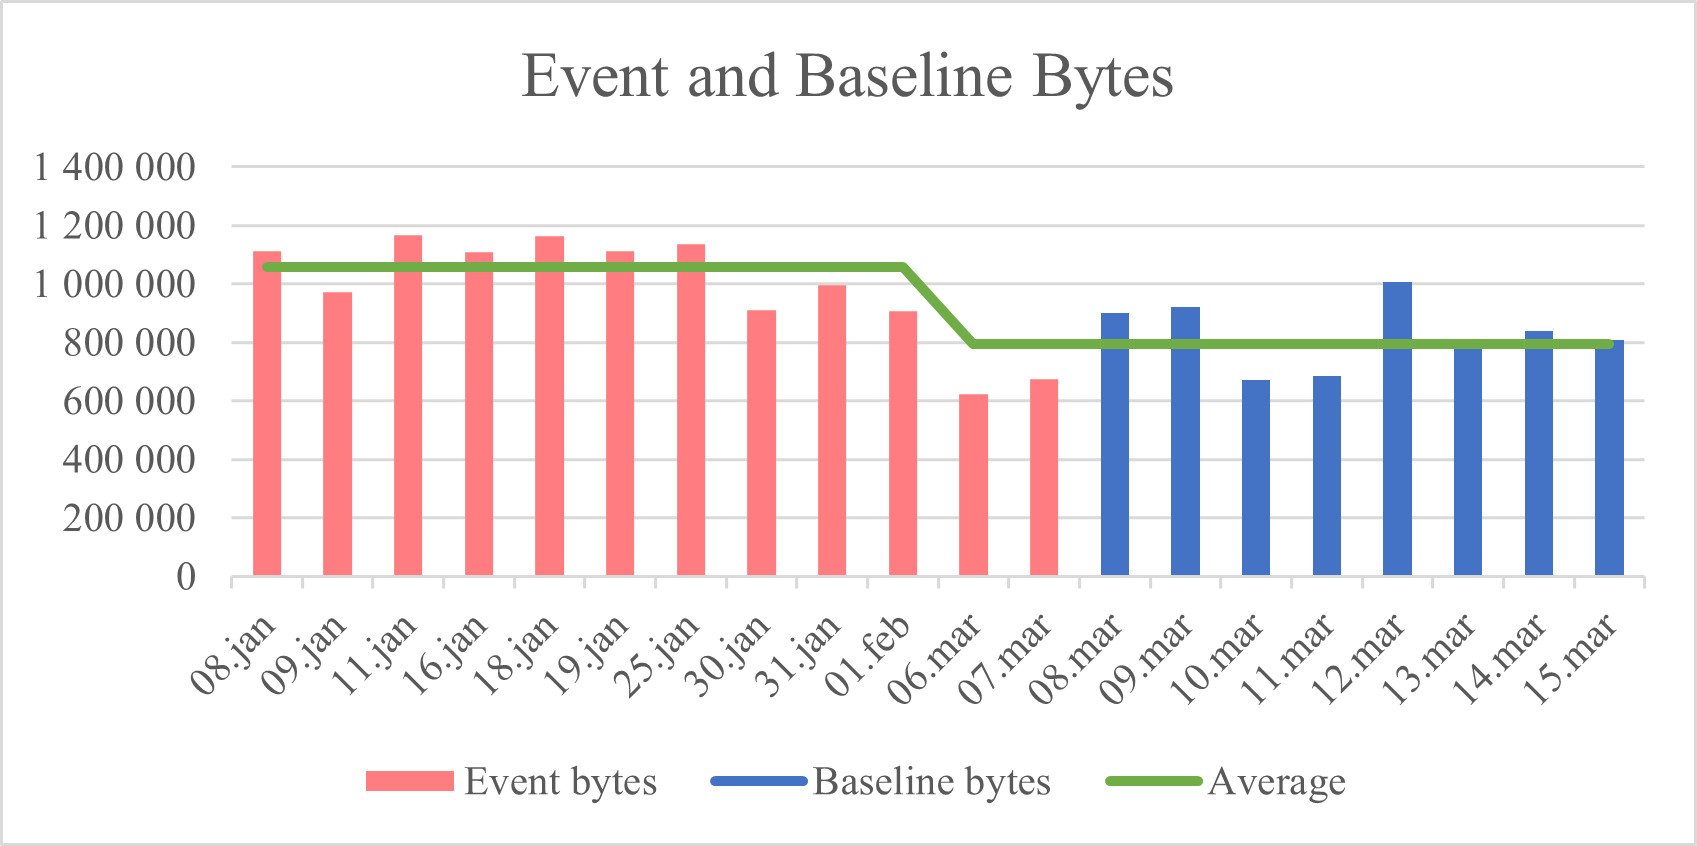
\includegraphics[width=1\hsize]{figures/Mill_Shower_Calculations_Bytes.png} 
    \end{subfigure}
    \begin{subfigure}{0.8\textwidth}
        \centering
        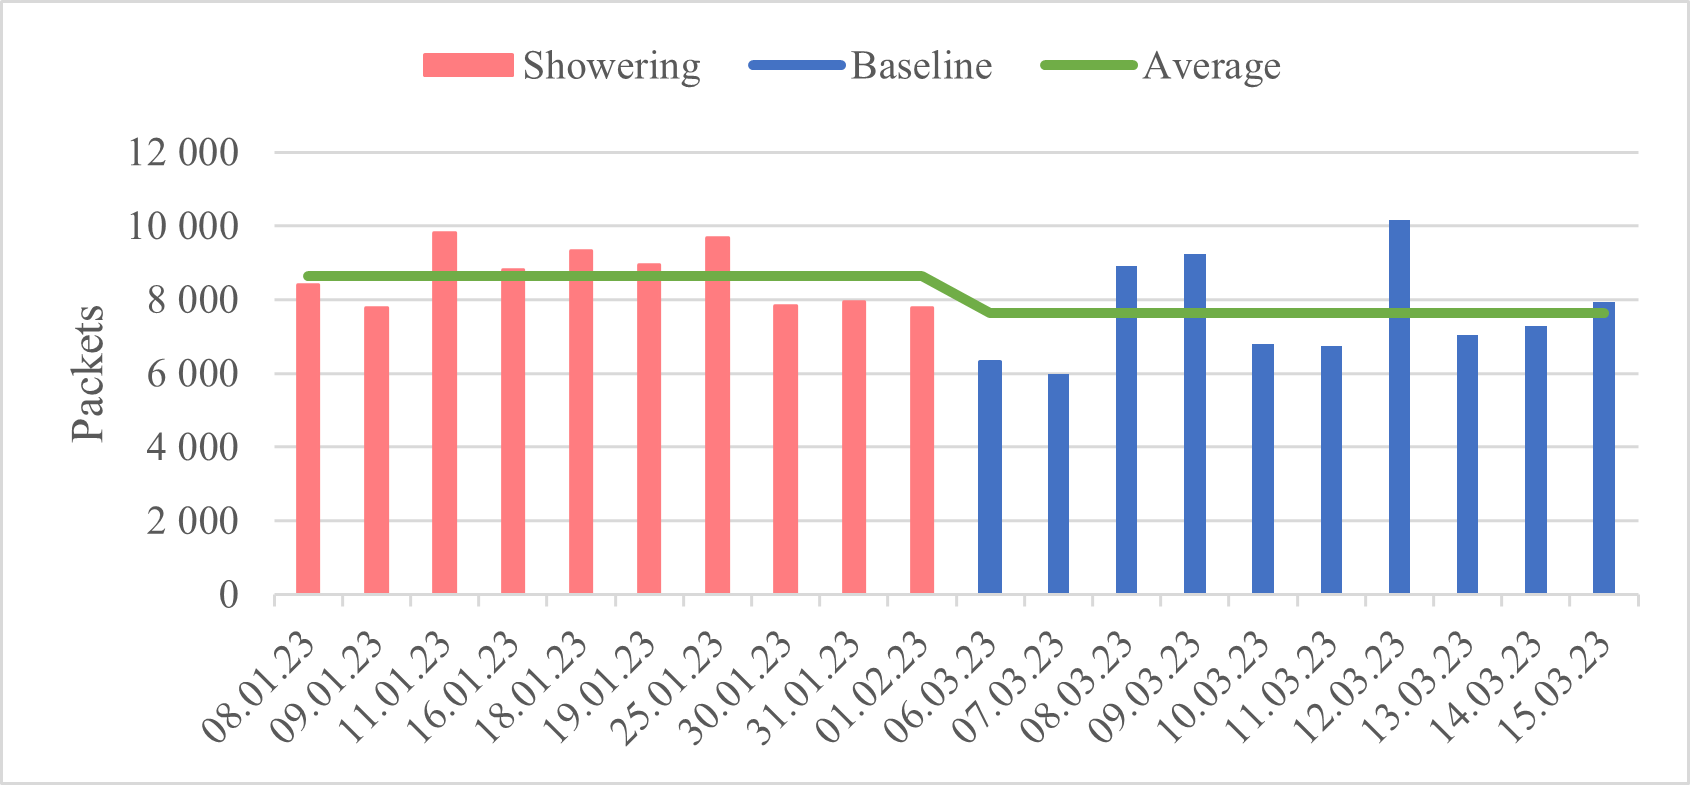
\includegraphics[width=1\hsize]{figures/Mill_Shower_Calculations_Packets.png} 
    \end{subfigure}
    \caption{Mill: Graphical presentation of event and baseline showering calculations with packets and bytes, including average value extracted from Table \ref{tab:NetatmoCookingCalculations}}
    \label{fig:MillShowerCalculations}
\end{figure}

Figure \ref{fig:MillShowerPackets1} and \ref{fig:MillShowerPackets2} shows the traffic flow during the events, placed on the left side of the figure and framed in red, and the baseline, placed on the right side of the figure and framed in blue, measured in number of packets. Figure \ref{fig:MillShowerBytes1} and \ref{fig:MillShowerBytes2} displays the same, but measured in number of bytes. The timings for when the event was ongoing are marked red on the event graphs. All graphs within the same figure have the same minimum and maximum values for the x- and y-axis. 

\begin{figure}[H]
    \begin{subfigure}[b]{0.47\textwidth}
        \centering
        \tcbincludegraphics[size=fbox,width=1.1\hsize,colframe=red]{figures/Mill_Shower_Packets_08.01.png}
    \end{subfigure}
    \begin{subfigure}[b]{0.47\textwidth}
        \centering
        \tcbincludegraphics[size=fbox,width=1.1\hsize, colframe=blue]{figures/Mill_Shower_Baseline_Packets_06.03.png}
    \end{subfigure}
    \begin{subfigure}[b]{0.47\textwidth}
        \centering
        \tcbincludegraphics[size=fbox,width=1.1\hsize,colframe=red]{figures/Mill_Shower_Packets_09.01.png}
    \end{subfigure}
    \begin{subfigure}[b]{0.47\textwidth}
        \centering
        \tcbincludegraphics[size=fbox,width=1.1\hsize,colframe=blue]{figures/Mill_Shower_Baseline_Packets_07.03.png}
    \end{subfigure}
    \begin{subfigure}[b]{0.47\textwidth}
        \centering
        \tcbincludegraphics[size=fbox,width=1.1\hsize,colframe=red]{figures/Mill_Shower_Packets_11.01.png}
    \end{subfigure}
    \begin{subfigure}[b]{0.47\textwidth}
        \centering
        \tcbincludegraphics[size=fbox,width=1.1\hsize,colframe=blue]{figures/Mill_Shower_Baseline_Packets_08.03.png}
    \end{subfigure}
    \begin{subfigure}[b]{0.47\textwidth}
        \centering
        \tcbincludegraphics[size=fbox,width=1.1\hsize,colframe=red]{figures/Mill_Shower_Packets_16.01.png}
    \end{subfigure}
    \begin{subfigure}[b]{0.47\textwidth}
        \centering
        \tcbincludegraphics[size=fbox,width=1.1\hsize,colframe=blue]{figures/Mill_Shower_Baseline_Packets_09.03.png}
    \end{subfigure}
    \begin{subfigure}[b]{0.47\textwidth}
        \centering
        \tcbincludegraphics[size=fbox,width=1.1\hsize,colframe=red]{figures/Mill_Shower_Packets_18.01.png}
    \end{subfigure}
    \begin{subfigure}[b]{0.47\textwidth}
        \centering
        \tcbincludegraphics[size=fbox,width=1.1\hsize,colframe=blue]{figures/Mill_Shower_Baseline_Packets_10.03.png}
    \end{subfigure}
        \begin{subfigure}[b]{0.47\textwidth}
        \centering
        \tcbincludegraphics[size=fbox,width=1.1\hsize,colframe=red]{figures/Mill_Shower_Packets_19.01.png}
    \end{subfigure}
    \begin{subfigure}[b]{0.47\textwidth}
        \centering
        \tcbincludegraphics[size=fbox,width=1.1\hsize,colframe=blue]{figures/Mill_Shower_Baseline_Packets_11.03.png}
    \end{subfigure}
    \begin{subfigure}[b]{0.47\textwidth}
        \centering
        \tcbincludegraphics[size=fbox,width=1.1\hsize,colframe=red]{figures/Mill_Shower_Packets_25.01.png}
    \end{subfigure}
    \hspace{0.6cm}
    \begin{subfigure}[b]{0.47\textwidth}
    \centering
        \tcbincludegraphics[size=fbox,width=1.1\hsize,colframe=blue]{figures/Mill_Shower_Baseline_Packets_12.03.png}
        \end{subfigure}
    \caption{Mill: Graphs of traffic flows in the shower events measured in packets with event graphs framed in red and baseline graphs framed in blue, Event times are marked in red on the event graphs.}
    \label{fig:MillShowerPackets1}
\end{figure}

\begin{figure}[H]
    \begin{subfigure}[b]{0.45\textwidth}
        \centering
        \tcbincludegraphics[size=fbox,width=1.1\hsize,colframe=red]{figures/Mill_Shower_Packets_30.01.png}
    \end{subfigure}
    \begin{subfigure}[b]{0.45\textwidth}
        \centering
        \tcbincludegraphics[size=fbox,width=1.1\hsize, colframe=blue]{figures/Mill_Shower_Baseline_Packets_13.03.png}
    \end{subfigure}
    \begin{subfigure}[b]{0.45\textwidth}
        \centering
        \tcbincludegraphics[size=fbox,width=1.1\hsize,colframe=red]{figures/Mill_Shower_Packets_31.01.png}
    \end{subfigure}
    \begin{subfigure}[b]{0.45\textwidth}
        \centering
        \tcbincludegraphics[size=fbox,width=1.1\hsize,colframe=blue]{figures/Mill_Shower_Baseline_Packets_14.03.png}
    \end{subfigure}
    \begin{subfigure}[b]{0.45\textwidth}
        \centering
        \tcbincludegraphics[size=fbox,width=1.1\hsize,colframe=red]{figures/Mill_Shower_Packets_01.02.png}
    \end{subfigure}
    \hspace{1.1cm}
    \begin{subfigure}[b]{0.45\textwidth}
        \centering
        \tcbincludegraphics[size=fbox,width=1.1\hsize,colframe=blue]{figures/Mill_Shower_Baseline_Packets_15.03.png}
    \end{subfigure}
    \caption{Mill: Continuing from Figure \ref{fig:MillShowerPackets1}}
    \label{fig:MillShowerPackets2}
\end{figure}

\begin{figure}[H]
    \begin{subfigure}[b]{0.45\textwidth}
        \centering
        \tcbincludegraphics[size=fbox,width=1.1\hsize,colframe=red]{figures/Mill_Shower_Bytes_30.01.png}
    \end{subfigure}
    \begin{subfigure}[b]{0.45\textwidth}
        \centering
        \tcbincludegraphics[size=fbox,width=1.1\hsize, colframe=blue]{figures/Mill_Shower_Baseline_Bytes_13.03.png}
    \end{subfigure}
    \begin{subfigure}[b]{0.45\textwidth}
        \centering
        \tcbincludegraphics[size=fbox,width=1.1\hsize,colframe=red]{figures/Mill_Shower_Bytes_31.01.png}
    \end{subfigure}
    \begin{subfigure}[b]{0.45\textwidth}
        \centering
        \tcbincludegraphics[size=fbox,width=1.1\hsize,colframe=blue]{figures/Mill_Shower_Baseline_Bytes_14.03.png}
    \end{subfigure}
    \begin{subfigure}[b]{0.45\textwidth}
        \centering
        \tcbincludegraphics[size=fbox,width=1.1\hsize,colframe=red]{figures/Mill_Shower_Bytes_01.02.png}
    \end{subfigure}
    \hspace{1.1cm}
    \begin{subfigure}[b]{0.45\textwidth}
        \centering
        \tcbincludegraphics[size=fbox,width=1.1\hsize,colframe=blue]{figures/Mill_Shower_Baseline_Bytes_15.03.png}
    \end{subfigure}
    \caption{Mill: Remaining graphs from Figure \ref{fig:MillShowerBytes2}}
    \label{fig:MillShowerBytes1}
\end{figure}

\begin{figure}[H]
    \begin{subfigure}[b]{0.47\textwidth}
        \centering
        \tcbincludegraphics[size=fbox,width=1.1\hsize,colframe=red]{figures/Mill_Shower_Bytes_08.01.png}
    \end{subfigure}
    \begin{subfigure}[b]{0.47\textwidth}
        \centering
        \tcbincludegraphics[size=fbox,width=1.1\hsize,colframe=blue]{figures/Mill_Shower_Baseline_Bytes_06.03.png}
    \end{subfigure}
    \begin{subfigure}[b]{0.47\textwidth}
        \centering
        \tcbincludegraphics[size=fbox,width=1.1\hsize,colframe=red]{figures/Mill_Shower_Bytes_09.01.png}
    \end{subfigure}
    \begin{subfigure}[b]{0.47\textwidth}
        \centering
        \tcbincludegraphics[size=fbox,width=1.1\hsize,colframe=blue]{figures/Mill_Shower_Baseline_Bytes_07.03.png}
    \end{subfigure}
    \begin{subfigure}[b]{0.47\textwidth}
        \centering
        \tcbincludegraphics[size=fbox,width=1.1\hsize,colframe=red]{figures/Mill_Shower_Bytes_11.01.png}
    \end{subfigure}
    \begin{subfigure}[b]{0.47\textwidth}
        \centering
        \tcbincludegraphics[size=fbox,width=1.1\hsize,colframe=blue]{figures/Mill_Shower_Baseline_Bytes_08.03.png}
    \end{subfigure}
    \begin{subfigure}[b]{0.47\textwidth}
        \centering
        \tcbincludegraphics[size=fbox,width=1.1\hsize,colframe=red]{figures/Mill_Shower_Bytes_16.01.png}
    \end{subfigure}
    \begin{subfigure}[b]{0.47\textwidth}
        \centering
        \tcbincludegraphics[size=fbox,width=1.1\hsize,colframe=blue]{figures/Mill_Shower_Baseline_Bytes_09.03.png}
    \end{subfigure}
    \begin{subfigure}[b]{0.47\textwidth}
        \centering
        \tcbincludegraphics[size=fbox,width=1.1\hsize,colframe=red]{figures/Mill_Shower_Bytes_18.01.png}
    \end{subfigure}
    \begin{subfigure}[b]{0.47\textwidth}
        \centering
        \tcbincludegraphics[size=fbox,width=1.1\hsize,colframe=blue]{figures/Mill_Shower_Baseline_Bytes_10.03.png}
    \end{subfigure}
        \begin{subfigure}[b]{0.47\textwidth}
        \centering
        \tcbincludegraphics[size=fbox,width=1.1\hsize,colframe=red]{figures/Mill_Shower_Bytes_19.01.png}
    \end{subfigure}
    \begin{subfigure}[b]{0.47\textwidth}
        \centering
        \tcbincludegraphics[size=fbox,width=1.1\hsize,colframe=blue]{figures/Mill_Shower_Baseline_Bytes_11.03.png}
    \end{subfigure}
    \begin{subfigure}[b]{0.47\textwidth}
        \centering
        \tcbincludegraphics[size=fbox,width=1.1\hsize,colframe=red]{figures/Mill_Shower_Bytes_25.01.png}
    \end{subfigure}
    \hspace{0.6cm}
    \begin{subfigure}[b]{0.47\textwidth}
    \centering
        \tcbincludegraphics[size=fbox,width=1.1\hsize,colframe=blue]{figures/Mill_Shower_Baseline_Bytes_12.03.png}
        \end{subfigure}
    \caption{Mill: Graphs of traffic flows in the shower events measured in bytes with event graphs framed in red and baseline graphs framed in blue, Event times are marked in red on the event graphs.}  
    \label{fig:MillShowerBytes2}
\end{figure}

Table \ref{tab:MillShowerCalculations} shows that the number of packets varies from 7,775 to 9,819 packets during the events compared to the baseline which varies from 5,968 to 10,151 packets shown in Table \ref{tab:MillBaselineShowerCalculations}. The baseline traffic has more variation than the event traffic. This also results in a higher standard deviation for the baseline shown in Table \ref{tab:MillComparingBaselineAndShowerCalculations}. For bytes, the same is shown, but the average value for the baseline is a lot smaller than for the events. As Table \ref{tab:MillBaselineShowerCalculations} shows, the bytes varies from 623,993 to 1,006,385 bytes, and in Table \ref{tab:MillShowerCalculations} the bytes varies from 909,992 to 1,166,768, which means that the average value for events are higher than for the baseline. Although the average value is higher, some of the baseline event days also measure similar amounts of bytes sent and received even tough an event is not ongoing. This is also confirmed in Figure \ref{fig:MillShowerCalculations} where bytes for baseline are much lower than for events, but there are also events that are lower than baseline days. 
\\\\
In the figures with packets, in Figure \ref{fig:MillShowerPackets1} and \ref{fig:MillShowerPackets2}, and bytes, in Figure \ref{fig:MillShowerBytes1} and \ref{fig:MillShowerBytes2} no distinct differences are visible in the graphical representation of the traffic flows. 

\newpage
\subsection{Nedis}
This subsection presents the results and analysis for Nedis during the showering event. The total amount of packets, bytes and the biggest packet during the packet captures are presented in Table \ref{tab:NedisShoweringCalculations} for the events and in Table \ref{tab:NedisBaselineShowerCalculations} for the corresponding baseline captures. Table \ref{tab:NedisComparingBaselineAndShowerCalculations} compares the average and standard deviation values calculated for the events and baseline. Figure \ref{fig:NedisShowerCalculations} shows a graphical presentation of the total number of bytes and packets during the events and baseline in the same figure with average values included.

\begin{table}[H]
\centering
    \caption{Nedis event calculations for the showering events}
\label{tab:NedisShoweringCalculations}
    \begin{tabular}{|l|l|l|l|}
        \hline
        \textbf{Events} & \textbf{Packets} & \textbf{Bytes} & \textbf{Biggest packet} \\ \hline
        08.jan          & 28,069           & 3,720,194      & 485 bytes               \\ \hline
        09.jan          & 23,156           & 3,395,004      & 424 bytes               \\ \hline
        11.jan          & 23,368           & 3,025,569      & 424 bytes               \\ \hline
        16.jan          & 21,026           & 2,598,912      & 485 bytes               \\ \hline
        18.jan          & 18,385           & 2,091,914      & 458 bytes               \\ \hline
        19.jan          & 25,416           & 3,258,851      & 421 bytes               \\ \hline
        25.jan          & 25,092           & 2,459,011      & 458 bytes               \\ \hline
        30.jan          & 22,415           & 3,302,325      & 485 bytes               \\ \hline
        31.jan          & 18,393           & 2,364,979      & 424 bytes               \\ \hline
        01.feb          & 20,306           & 2,461,409      & 485 bytes               \\ \hline
    \end{tabular}
\end{table}

\begin{table}[H]
    \centering
    \caption{Nedis baseline calculations for the corresponding showering event times}
    \begin{tabular}{|l|l|l|l|l|l|}
    \hline
        \textbf{Baseline} & \textbf{Packets} & \textbf{Bytes} & \textbf{Biggest packet} \\ \hline
        06.mar & 12,495 & 1,534,872 & 522 bytes \\ \hline
        07.mar & 18,342 & 2,483,719 & 522 bytes \\ \hline
        08.mar & 18,318 & 2,116,146 & 424 bytes \\ \hline
        09.mar & 14,639 & 1,865,223 & 522 bytes \\ \hline
        10.mar & 9,893  & 1,434,033 & 522 bytes \\ \hline
        11.mar & 6,092  & 779,215   & 426 bytes \\ \hline
        12.mar & 10,736 & 1,273,551 & 426 bytes \\ \hline
        13.mar & 13,478 & 1,649,747 & 424 bytes \\ \hline
        14.mar & 14,239 & 1,668,084 & 522 bytes \\ \hline
        15.mar & 22,383 & 2,710,729 & 522 bytes \\ \hline
    \end{tabular}
    \label{tab:NedisBaselineShowerCalculations}
\end{table}

\begin{table}[H]
    \centering
    \caption{Nedis: Comparing event and baseline calculations for the showering test}
    \begin{tabular}{c|l|l|l|l|}
        \cline{2-5}
        \multicolumn{1}{l|}{}                                              & \textbf{Type} & \textbf{Packets} & \textbf{Bytes} & \textbf{Biggest packet} \\ \hline
        \multicolumn{1}{|c|}{\multirow{2}{*}{\textbf{Average}}}            & Event         & 22,563             & 2,867,817       & 455 bytes               \\ \cline{2-5} 
        \multicolumn{1}{|c|}{}                                             & Baseline      & 14,062             & 1,752,432       & 483 bytes                \\ \hline
        \multicolumn{1}{|c|}{\multirow{2}{*}{\textbf{Standard deviation}}} & Event         & 3,130              & 540,631         & 29 bytes                 \\ \cline{2-5} 
        \multicolumn{1}{|c|}{}                                             & Baseline      & 4,723              & 571,269         & 50 bytes               \\ \hline          
    \end{tabular}
    \label{tab:NedisComparingBaselineAndShowerCalculations}
\end{table}

\begin{figure}[H]
    \centering
    \begin{subfigure}{0.8\textwidth}
        \centering
        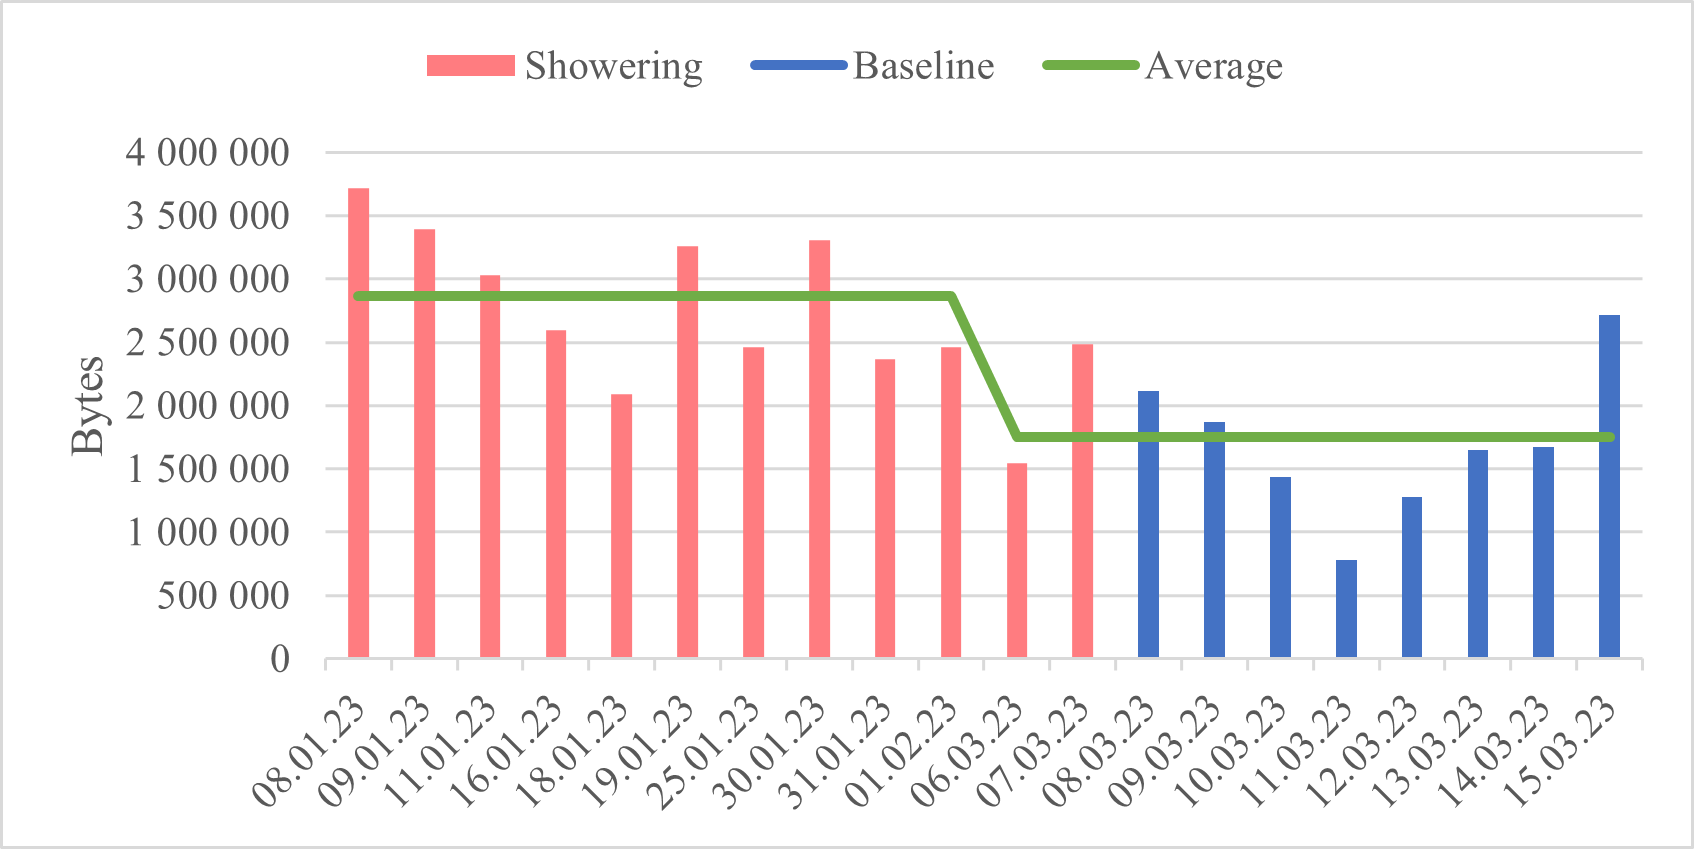
\includegraphics[width=1\hsize]{figures/Nedis_Shower_Calculations_Bytes.png} 
    \end{subfigure}
    \begin{subfigure}{0.8\textwidth}
        \centering
        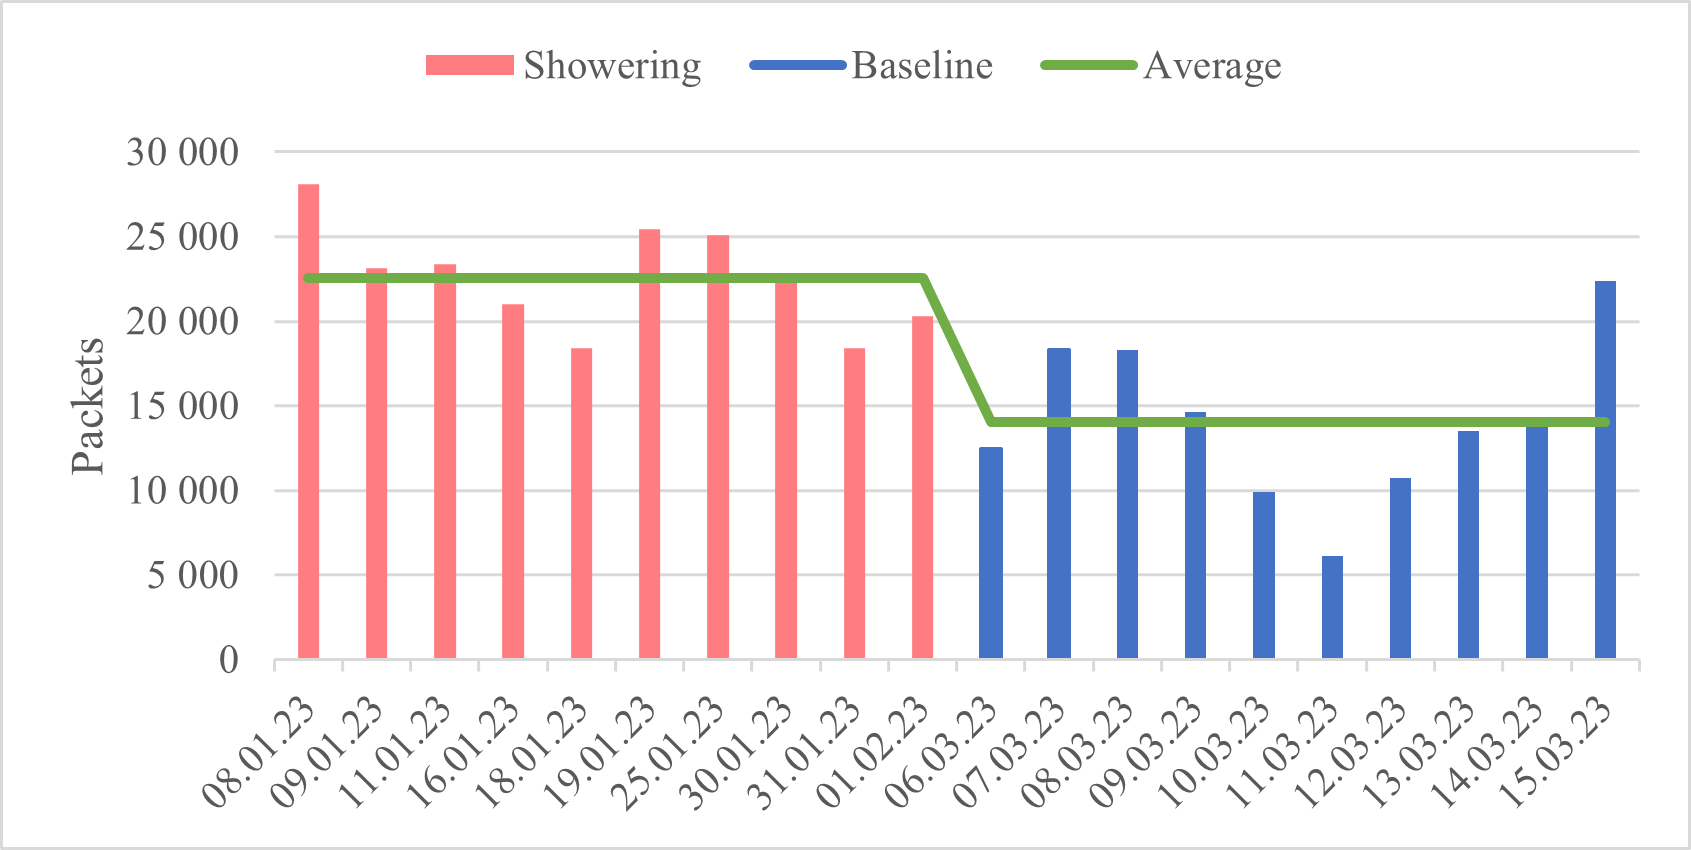
\includegraphics[width=1\hsize]{figures/Nedis_Shower_Calculations_Packets.png} 
    \end{subfigure}
    \caption{Nedis: Graphical presentation of event and baseline showering calculations with packets and bytes, including average value extracted from Table \ref{tab:NetatmoCookingCalculations}}
    \label{fig:NedisShowerCalculations}
\end{figure}

In Figure \ref{fig:NedisShowerPackets1} and \ref{fig:NedisShowerPackets2} a graphical presentation of the traffic flow measured in number of packets are displayed. The same view is presented in Figure \ref{fig:NedisShowerBytes1} and \ref{fig:NedisShowerBytes2} with number of bytes as the y-axis. Both of theses figures have the event graphs placed on the left side of the figure framed in red, while the baseline graphs are placed on the right side of the figure framed in blue to compare to each other. The time of the events are marked red on all of the event graphs. The x- and y-axis have the same minimum and maximum values for all graphs within the same figure. 

\begin{figure}[H]
    \begin{subfigure}[b]{0.47\textwidth}
        \centering
        \tcbincludegraphics[size=fbox,width=1.1\hsize,colframe=red]{figures/Nedis_Shower_Packets_08.01.png}
    \end{subfigure}
    \begin{subfigure}[b]{0.47\textwidth}
        \centering
        \tcbincludegraphics[size=fbox,width=1.1\hsize, colframe=blue]{figures/Nedis_Shower_Baseline_Packets_06.03.png}
    \end{subfigure}
    \begin{subfigure}[b]{0.47\textwidth}
        \centering
        \tcbincludegraphics[size=fbox,width=1.1\hsize,colframe=red]{figures/Nedis_Shower_Packets_09.01.png}
    \end{subfigure}
    \begin{subfigure}[b]{0.47\textwidth}
        \centering
        \tcbincludegraphics[size=fbox,width=1.1\hsize,colframe=blue]{figures/Nedis_Shower_Baseline_Packets_07.03.png}
    \end{subfigure}
    \begin{subfigure}[b]{0.47\textwidth}
        \centering
        \tcbincludegraphics[size=fbox,width=1.1\hsize,colframe=red]{figures/Nedis_Shower_Packets_11.01.png}
    \end{subfigure}
    \begin{subfigure}[b]{0.47\textwidth}
        \centering
        \tcbincludegraphics[size=fbox,width=1.1\hsize,colframe=blue]{figures/Nedis_Shower_Baseline_Packets_08.03.png}
    \end{subfigure}
    \begin{subfigure}[b]{0.47\textwidth}
        \centering
        \tcbincludegraphics[size=fbox,width=1.1\hsize,colframe=red]{figures/Nedis_Shower_Packets_16.01.png}
    \end{subfigure}
    \begin{subfigure}[b]{0.47\textwidth}
        \centering
        \tcbincludegraphics[size=fbox,width=1.1\hsize,colframe=blue]{figures/Nedis_Shower_Baseline_Packets_09.03.png}
    \end{subfigure}
    \begin{subfigure}[b]{0.47\textwidth}
        \centering
        \tcbincludegraphics[size=fbox,width=1.1\hsize,colframe=red]{figures/Nedis_Shower_Packets_18.01.png}
    \end{subfigure}
    \begin{subfigure}[b]{0.47\textwidth}
        \centering
        \tcbincludegraphics[size=fbox,width=1.1\hsize,colframe=blue]{figures/Nedis_Shower_Baseline_Packets_10.03.png}
    \end{subfigure}
        \begin{subfigure}[b]{0.47\textwidth}
        \centering
        \tcbincludegraphics[size=fbox,width=1.1\hsize,colframe=red]{figures/Nedis_Shower_Packets_19.01.png}
    \end{subfigure}
    \begin{subfigure}[b]{0.47\textwidth}
        \centering
        \tcbincludegraphics[size=fbox,width=1.1\hsize,colframe=blue]{figures/Nedis_Shower_Baseline_Packets_11.03.png}
    \end{subfigure}
    \begin{subfigure}[b]{0.47\textwidth}
        \centering
        \tcbincludegraphics[size=fbox,width=1.1\hsize,colframe=red]{figures/Nedis_Shower_Packets_25.01.png}
    \end{subfigure}
    \hspace{0.6cm}
    \begin{subfigure}[b]{0.47\textwidth}
    \centering
        \tcbincludegraphics[size=fbox,width=1.1\hsize,colframe=blue]{figures/Nedis_Shower_Baseline_Packets_12.03.png}
        \end{subfigure}
    \caption{Nedis: Graphs of traffic flows in the shower events measured in packets with event graphs framed in red and baseline graphs framed in blue, Event times are marked in red on the event graphs.}
    \label{fig:NedisShowerPackets1}
\end{figure}

\begin{figure}[H]
    \begin{subfigure}[b]{0.45\textwidth}
        \centering
        \tcbincludegraphics[size=fbox,width=1.1\hsize,colframe=red]{figures/Nedis_Shower_Packets_30.01.png}
    \end{subfigure}
    \begin{subfigure}[b]{0.45\textwidth}
        \centering
        \tcbincludegraphics[size=fbox,width=1.1\hsize, colframe=blue]{figures/Nedis_Shower_Baseline_Packets_13.03.png}
    \end{subfigure}
    \begin{subfigure}[b]{0.45\textwidth}
        \centering
        \tcbincludegraphics[size=fbox,width=1.1\hsize,colframe=red]{figures/Nedis_Shower_Packets_31.01.png}
    \end{subfigure}
    \begin{subfigure}[b]{0.45\textwidth}
        \centering
        \tcbincludegraphics[size=fbox,width=1.1\hsize,colframe=blue]{figures/Nedis_Shower_Baseline_Packets_14.03.png}
    \end{subfigure}
    \begin{subfigure}[b]{0.45\textwidth}
        \centering
        \tcbincludegraphics[size=fbox,width=1.1\hsize,colframe=red]{figures/Nedis_Shower_Packets_01.02.png}
    \end{subfigure}
    \hspace{1.1cm}
    \begin{subfigure}[b]{0.45\textwidth}
        \centering
        \tcbincludegraphics[size=fbox,width=1.1\hsize,colframe=blue]{figures/Nedis_Shower_Baseline_Packets_15.03.png}
    \end{subfigure}
    \caption{Nedis: Continuing from Figure \ref{fig:NedisShowerPackets1}}
    \label{fig:NedisShowerPackets2}
\end{figure}

\begin{figure}[H]
    \begin{subfigure}[b]{0.45\textwidth}
        \centering
        \tcbincludegraphics[size=fbox,width=1.1\hsize,colframe=red]{figures/Nedis_Shower_Bytes_30.01.png}
    \end{subfigure}
    \begin{subfigure}[b]{0.45\textwidth}
        \centering
        \tcbincludegraphics[size=fbox,width=1.1\hsize, colframe=blue]{figures/Nedis_Shower_Baseline_Bytes_13.03.png}
    \end{subfigure}
    \begin{subfigure}[b]{0.45\textwidth}
        \centering
        \tcbincludegraphics[size=fbox,width=1.1\hsize,colframe=red]{figures/Nedis_Shower_Bytes_31.01.png}
    \end{subfigure}
    \begin{subfigure}[b]{0.45\textwidth}
        \centering
        \tcbincludegraphics[size=fbox,width=1.1\hsize,colframe=blue]{figures/Nedis_Shower_Baseline_Bytes_14.03.png}
    \end{subfigure}
    \begin{subfigure}[b]{0.45\textwidth}
        \centering
        \tcbincludegraphics[size=fbox,width=1.1\hsize,colframe=red]{figures/Nedis_Shower_Bytes_01.02.png}
    \end{subfigure}
    \hspace{1.1cm}
    \begin{subfigure}[b]{0.45\textwidth}
        \centering
        \tcbincludegraphics[size=fbox,width=1.1\hsize,colframe=blue]{figures/Nedis_Shower_Baseline_Bytes_15.03.png}
    \end{subfigure}
    \caption{Nedis: Remaining graphs from Figure \ref{fig:NedisShowerBytes2}}
    \label{fig:NedisShowerBytes1}
\end{figure}

\begin{figure}[H]
    \begin{subfigure}[b]{0.47\textwidth}
        \centering
        \tcbincludegraphics[size=fbox,width=1.1\hsize,colframe=red]{figures/Nedis_Shower_Bytes_08.01.png}
    \end{subfigure}
    \begin{subfigure}[b]{0.47\textwidth}
        \centering
        \tcbincludegraphics[size=fbox,width=1.1\hsize,colframe=blue]{figures/Nedis_Shower_Baseline_Bytes_06.03.png}
    \end{subfigure}
    \begin{subfigure}[b]{0.47\textwidth}
        \centering
        \tcbincludegraphics[size=fbox,width=1.1\hsize,colframe=red]{figures/Nedis_Shower_Bytes_09.01.png}
    \end{subfigure}
    \begin{subfigure}[b]{0.47\textwidth}
        \centering
        \tcbincludegraphics[size=fbox,width=1.1\hsize,colframe=blue]{figures/Nedis_Shower_Baseline_Bytes_07.03.png}
    \end{subfigure}
    \begin{subfigure}[b]{0.47\textwidth}
        \centering
        \tcbincludegraphics[size=fbox,width=1.1\hsize,colframe=red]{figures/Nedis_Shower_Bytes_11.01.png}
    \end{subfigure}
    \begin{subfigure}[b]{0.47\textwidth}
        \centering
        \tcbincludegraphics[size=fbox,width=1.1\hsize,colframe=blue]{figures/Nedis_Shower_Baseline_Bytes_08.03.png}
    \end{subfigure}
    \begin{subfigure}[b]{0.47\textwidth}
        \centering
        \tcbincludegraphics[size=fbox,width=1.1\hsize,colframe=red]{figures/Nedis_Shower_Bytes_16.01.png}
    \end{subfigure}
    \begin{subfigure}[b]{0.47\textwidth}
        \centering
        \tcbincludegraphics[size=fbox,width=1.1\hsize,colframe=blue]{figures/Nedis_Shower_Baseline_Bytes_09.03.png}
    \end{subfigure}
    \begin{subfigure}[b]{0.47\textwidth}
        \centering
        \tcbincludegraphics[size=fbox,width=1.1\hsize,colframe=red]{figures/Nedis_Shower_Bytes_18.01.png}
    \end{subfigure}
    \begin{subfigure}[b]{0.47\textwidth}
        \centering
        \tcbincludegraphics[size=fbox,width=1.1\hsize,colframe=blue]{figures/Nedis_Shower_Baseline_Bytes_10.03.png}
    \end{subfigure}
        \begin{subfigure}[b]{0.47\textwidth}
        \centering
        \tcbincludegraphics[size=fbox,width=1.1\hsize,colframe=red]{figures/Nedis_Shower_Bytes_19.01.png}
    \end{subfigure}
    \begin{subfigure}[b]{0.47\textwidth}
        \centering
        \tcbincludegraphics[size=fbox,width=1.1\hsize,colframe=blue]{figures/Nedis_Shower_Baseline_Bytes_11.03.png}
    \end{subfigure}
    \begin{subfigure}[b]{0.47\textwidth}
        \centering
        \tcbincludegraphics[size=fbox,width=1.1\hsize,colframe=red]{figures/Nedis_Shower_Bytes_25.01.png}
    \end{subfigure}
    \hspace{0.6cm}
    \begin{subfigure}[b]{0.47\textwidth}
    \centering
        \tcbincludegraphics[size=fbox,width=1.1\hsize,colframe=blue]{figures/Nedis_Shower_Baseline_Bytes_12.03.png}
        \end{subfigure}
    \caption{Nedis: Graphs of traffic flows in the shower events measured in bytes with event graphs framed in red and baseline graphs framed in blue, Event times are marked in red on the event graphs.}  
    \label{fig:NedisShowerBytes2}
\end{figure}

Comparing the values for both packets and bytes in Figure \ref{tab:NedisShoweringCalculations} and \ref{tab:NedisBaselineShowerCalculations} shows that during the events, most of the values are a lot higher than for the baseline calculations. For event, the packets varies from 18,385 to 28,069 and bytes from 2,091,914 to 3,720,194 bytes. However, there are values from the baseline that matches the range of the event values, such as for 7th, 8th and 15th of March where the values for packets are over 18,000 and 2,000,000 for bytes. For the biggest packet sent, the baseline have a higher overall value compared to the event values, where baseline are mostly around 500 bytes and events are lower than 500 bytes for every day. The average values also shows that the event values are higher than the baseline values for both packets and bytes. The difference in both average values and overall for events and baseline are significantly shown in Figure \ref{fig:NedisShowerCalculations} where both packets and bytes are much lower for baseline than events. 
\\\\
Looking at the graphs in Figure \ref{fig:NedisShowerPackets1} and \ref{fig:NedisShowerPackets2} the difference in number of packets are visible. However, it does not look like the number of packets changes when the shower event starts, but are just higher during several of those days. In these figures, one can also see that some of the baseline days looks similar as the event calculations in the tables. For bytes in Figure \ref{fig:NedisShowerBytes1} and \ref{fig:NedisShowerBytes2}, the results gives the same result as for packets. 

\newpage
\section{Test Case 3: Window Open}
This chapter presents the results and analysis conducted on Test Case 3: Window Open. 
\subsection{General}
Test case 3: Window Open has been conducted 10 times over the course of 10 different days. The days and timings for the events are presented in Table \ref{tab:WindowDates}.

\begin{table}[H]
    \centering
    \caption{Date and time for Test Case 3: Window Open events}
    \begin{adjustbox}{width=1\textwidth} 
            \begin{tabular}{l|l|l|l|l|l|l|l|l|l|l|}
                \cline{2-11}
                & 08.01 & 09.01 & 11.01 & 16.01 & 18.01 & 19.01 & 25.01 & 30.01 & 31.01 & 01.02 \\ \hline
                \multicolumn{1}{|l|}{Started event}  & 23:00 & 23:00 & 22:50 & 23:10 & 23:15 & 23:02 & 22:59 & 23:00 & 22:59 & 22:59 \\ \hline
                \multicolumn{1}{|l|}{Finished event} & 07:00 & 07:00 & 07:00 & 06:56 & 07:09 & 06:59 & 06:55 & 06:56 & 07:00 & 06:59 \\ \hline
            \end{tabular}
    \end{adjustbox}
    \label{tab:WindowDates}
\end{table}

To be able to compare the events to standby traffic, the baseline capture has been used within the same timings as for the actual events. To easier compare the events with each other and against the baseline, all packet captures have been filtered with the same start and finish time. Due to time limitations, the baseline only includes 9 full nights and therefore only 9 corresponding baseline packet captures have been made and used for comparison in this section. To ensure that all events have at least 30 minutes before and after the event was ongoing, the earliest time for starting and the latest time for finishing the event has been used to calculate the start and finish times for the files. Then 30 minutes are added to these times to ensure that each event has at least 30 minutes before and after to see traffic changes. The timings are extracted from Table \ref{tab:WindowDates} and presented in the list beneath: 

\begin{itemize}
    \item Earliest Event Start: 22:50
    \item Latest Event Finished: 07:09
    \item Packet Capture Files Start: 22:20
    \item Packet Capture Files End: 07:39
\end{itemize}

These times results in the following filters added to create the pcaps for each event:
\begin{itemize}
    \item frame.time >= "Month Date, Year 22:20:00" \&\& frame.time <= "Month Date, Year 07:39:00"
\end{itemize}

The next subsections presents the results and analysis for the three different devices, Netatmo, Mill and Nedis. As they are all equal in their setup of presenting the results, an explanation are included here instead of at the beginning of each sub-section for each device. The results are presented both graphically and with calculations. The calculations are presented in three different tables and in one figure, while the graphical presentations are included in the rest of the figures in the sub-sections. The first two tables in each subsection includes the total amount of packet and bytes sent and received to that particular device during the event with the last column including an extract of the biggest packet during the packet captures, regardless of if its sent or received by the device. These tables presents the values for each of the event and baseline dates for the device. The next table, presents the average and standard deviation values from the first two tables with all the columns included to easier compare the two to each other. Then a figure is used to present the total number of bytes and packets sent and received from the device for each of the event and baseline files in the same figure. The average values are also included here. 
\\\\
Each device then has a graphical presentation of the traffic flow presented in four different figures. The first two figures are with the amount of packets as the scale on the y-axis, while the two last are with the amount of bytes as the scale on the y-axis. All figures within the same category, meaning packet or bytes for a specific device has the same minimum and maximum values for bytes or packets on the y-axis and the same start and finish time on the x-axis. To be able to compare events against baseline, both traffic flows are included in the same figure, where events are placed on the left side while baseline are placed on the right side of every figure. The events are framed in a red color and the baseline in a blue color to be able to separate them even further. At the end of each sub-section, a few paragraphs are given to comment on the results and show the analysis. 

\newpage
\subsection{Netatmo}

\begin{table}[H]
    \centering
    \caption{Netatmo event calculations for the window open events}
    \begin{tabular}{|l|l|l|l|l|l|}
    \hline
        \textbf{Event dates} & \textbf{Packets} & \textbf{Bytes} & \textbf{Biggest packet} \\ \hline
        08.jan & 4,716 & 641,245 & 407 bytes\\ \hline
        09.jan & 4,026 & 544,344 & 407 bytes \\ \hline
        11.jan & 5,149 & 697,920 & 407 bytes\\ \hline
        16.jan & 4,493 & 608,029 & 407 bytes\\ \hline
        18.jan & 4,165 & 565,885 & 407 bytes\\ \hline
        19.jan & 3,877 & 527,113 & 407 bytes \\ \hline
        25.jan & 4,460 & 605,296 & 407 bytes \\ \hline
        30.jan & 3,745 & 509,093 & 407 bytes \\ \hline
        31.jan & 3,494 & 468,922 & 407 bytes \\ \hline
        01.feb & 3,858 & 522,632 & 407 bytes \\ \hline
    \end{tabular}
    \label{tab:NetatmoWindowCalculations}
\end{table}

\begin{table}[H]
    \centering
    \caption{Netatmo baseline calculations for the corresponding window open event times}
    \begin{tabular}{|l|l|l|l|}
    \hline
        \textbf{Baseline} & \textbf{Packets} & \textbf{Bytes} & \textbf{Biggest packet} \\ \hline
        06.mar & 3,447 & 460,531 & 387 bytes\\ \hline
        07.mar & 4,356 & 591,234 & 407 bytes\\ \hline
        08.mar & 4,373 & 587,975 & 407 bytes \\ \hline
        09.mar & 4,513 & 609,590 & 407 bytes \\ \hline
        10.mar & 4,637 & 631,232 & 407 bytes \\ \hline
        11.mar & 4,010 & 545,391 & 407 bytes \\ \hline
        12.mar & 3,815 & 520,289 & 407 bytes \\ \hline
        13.mar & 3,571 & 478,194 & 407 bytes \\ \hline
        14.mar & 3,716 & 503,515 & 407 bytes \\ \hline
    \end{tabular}
    \label{tab:NetatmoBaselineWindowCalculations}
\end{table}

\begin{table}[H]
    \centering
    \caption{Netatmo: Comparing event and baseline calculations for the window open test}
    \begin{tabular}{c|l|l|l|l|}
        \cline{2-5}
        \multicolumn{1}{l|}{}                                              & \textbf{Type} & \textbf{Packets} & \textbf{Bytes} & \textbf{Biggest packet} \\ \hline
        \multicolumn{1}{|c|}{\multirow{2}{*}{\textbf{Average}}}            & Event         & 4,198            & 569,048        & 407 bytes               \\ \cline{2-5} 
        \multicolumn{1}{|c|}{}                                             & Baseline      & 4,049            & 547,550        & 405 bytes                \\ \hline
        \multicolumn{1}{|c|}{\multirow{2}{*}{\textbf{Standard deviation}}} & Event         & 503              & 68,966         & 0 bytes                 \\ \cline{2-5} 
        \multicolumn{1}{|c|}{}                                             & Baseline      & 436              & 60,687         & 7 bytes               \\ \hline          
    \end{tabular}
    \label{tab:NetatmoComparingBaselineAndWindowCalculations}
\end{table}

\begin{figure}[H]
    \centering
    \begin{subfigure}{0.8\textwidth}
       \centering
       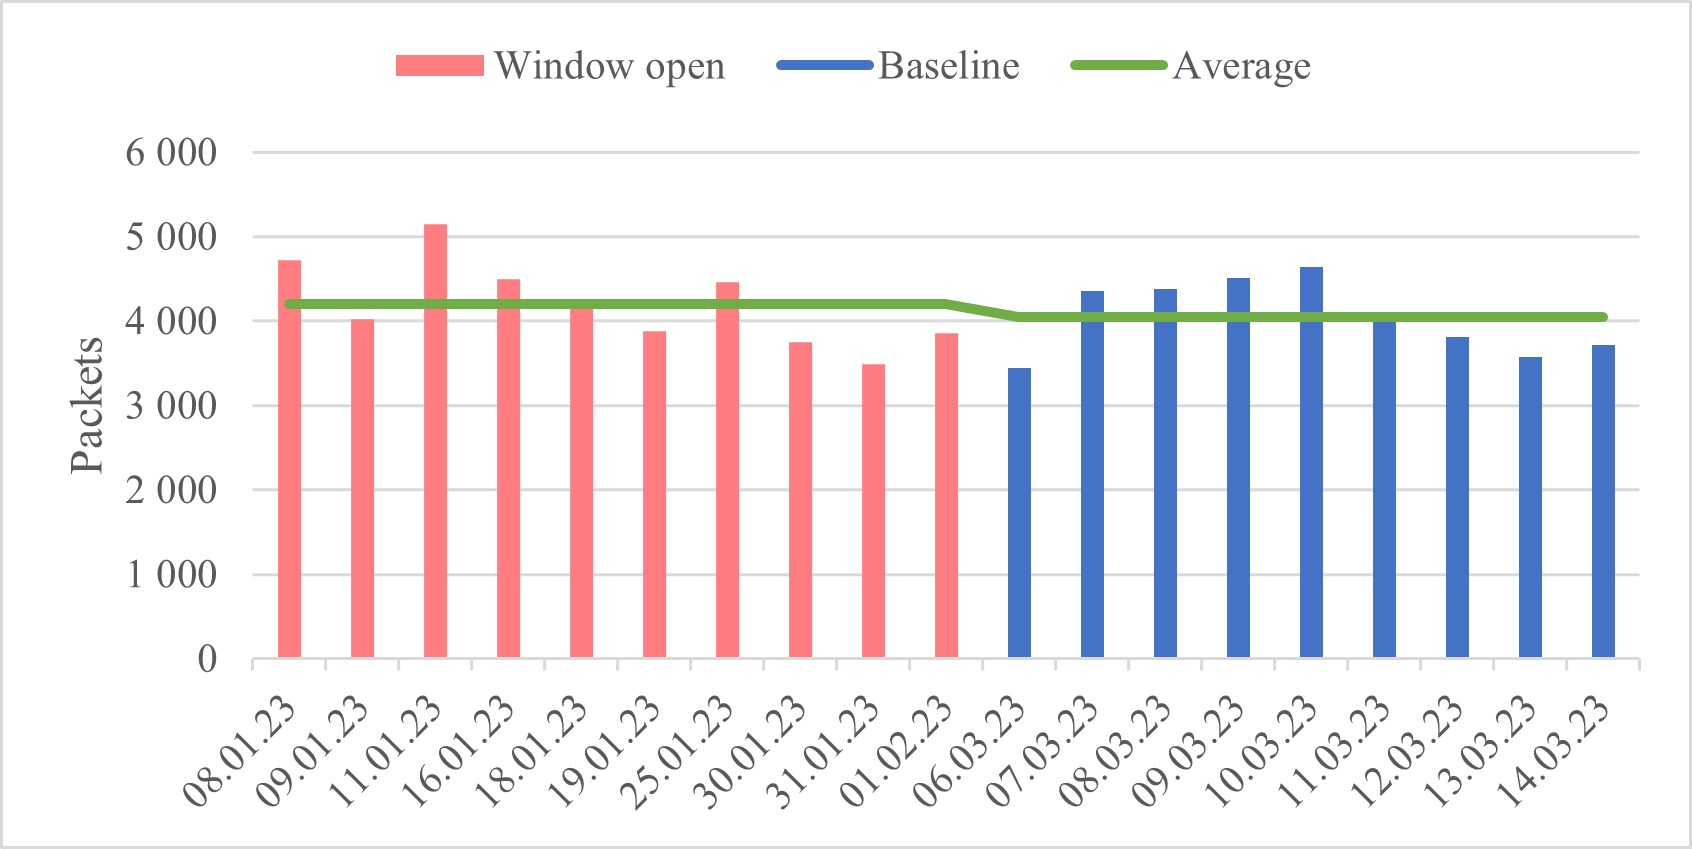
\includegraphics[width=1\hsize]{figures/Netatmo_Window_Calculations_Packets.png} 
    \end{subfigure}
    \begin{subfigure}{0.8\textwidth}
        \centering
        \includegraphics[width=1\hsize]{figures/Netatmo_Window_Calculations_Bytes.png} 
    \end{subfigure}
    \caption{Netatmo: Graphical presentation of event and baseline window open calculations with packets and bytes, including average value extracted from Table \ref{tab:NetatmoCookingCalculations}}
    \label{fig:NetatmoWindowCalculations}
\end{figure}

\begin{figure}[H]
    \begin{subfigure}[b]{0.47\textwidth}
        \centering
        \tcbincludegraphics[size=fbox,width=1.1\hsize,colframe=red]{figures/Netatmo_Window_Packets_08.01-09.01.png}
    \end{subfigure}
    \begin{subfigure}[b]{0.47\textwidth}
        \centering
        \tcbincludegraphics[size=fbox,width=1.1\hsize, colframe=blue]{figures/Netatmo_Window_Baseline_Packets_06.03-07.03.png}
    \end{subfigure}
    \begin{subfigure}[b]{0.47\textwidth}
        \centering
        \tcbincludegraphics[size=fbox,width=1.1\hsize,colframe=red]{figures/Netatmo_Window_Packets_09.01-10.01.png}
    \end{subfigure}
    \begin{subfigure}[b]{0.47\textwidth}
        \centering
        \tcbincludegraphics[size=fbox,width=1.1\hsize,colframe=blue]{figures/Netatmo_Window_Baseline_Packets_07.03-08.03.png}
    \end{subfigure}
    \begin{subfigure}[b]{0.47\textwidth}
        \centering
        \tcbincludegraphics[size=fbox,width=1.1\hsize,colframe=red]{figures/Netatmo_Window_Packets_11.01-12.01.png}
    \end{subfigure}
    \begin{subfigure}[b]{0.47\textwidth}
        \centering
        \tcbincludegraphics[size=fbox,width=1.1\hsize,colframe=blue]{figures/Netatmo_Window_Baseline_Packets_08.03-09.03.png}
    \end{subfigure}
    \begin{subfigure}[b]{0.47\textwidth}
        \centering
        \tcbincludegraphics[size=fbox,width=1.1\hsize,colframe=red]{figures/Netatmo_Window_Packets_16.01-17.01.png}
    \end{subfigure}
    \begin{subfigure}[b]{0.47\textwidth}
        \centering
        \tcbincludegraphics[size=fbox,width=1.1\hsize,colframe=blue]{figures/Netatmo_Window_Baseline_Packets_09.03-10.03.png}
    \end{subfigure}
    \begin{subfigure}[b]{0.47\textwidth}
        \centering
        \tcbincludegraphics[size=fbox,width=1.1\hsize,colframe=red]{figures/Netatmo_Window_Packets_18.01-19.01.png}
    \end{subfigure}
    \begin{subfigure}[b]{0.47\textwidth}
        \centering
        \tcbincludegraphics[size=fbox,width=1.1\hsize,colframe=blue]{figures/Netatmo_Window_Baseline_Packets_10.03-11.03.png}
    \end{subfigure}
        \begin{subfigure}[b]{0.47\textwidth}
        \centering
        \tcbincludegraphics[size=fbox,width=1.1\hsize,colframe=red]{figures/Netatmo_Window_Packets_19.01-20.01.png}
    \end{subfigure}
    \begin{subfigure}[b]{0.47\textwidth}
        \centering
        \tcbincludegraphics[size=fbox,width=1.1\hsize,colframe=blue]{figures/Netatmo_Window_Baseline_Packets_11.03-12.03.png}
    \end{subfigure}
    \begin{subfigure}[b]{0.47\textwidth}
        \centering
        \tcbincludegraphics[size=fbox,width=1.1\hsize,colframe=red]{figures/Netatmo_Window_Packets_25.01-26.01.png}
    \end{subfigure}
    \hspace{0.6cm}
    \begin{subfigure}[b]{0.47\textwidth}
    \centering
        \tcbincludegraphics[size=fbox,width=1.1\hsize,colframe=blue]{figures/Netatmo_Window_Baseline_Packets_12.03-13.03.png}
        \end{subfigure}
    \caption{Netatmo: Graphs of traffic flows in the window open events measured in packets with event graphs framed in red and baseline graphs framed in blue, Event times are marked in red on the event graphs.}
    \label{fig:NetatmoWindowPackets1}
\end{figure}

\begin{figure}[H]
    \begin{subfigure}[b]{0.45\textwidth}
        \centering
        \tcbincludegraphics[size=fbox,width=1.1\hsize,colframe=red]{figures/Netatmo_Window_Packets_30.01-31.01.png}
    \end{subfigure}
    \begin{subfigure}[b]{0.45\textwidth}
        \centering
        \tcbincludegraphics[size=fbox,width=1.1\hsize, colframe=blue]{figures/Netatmo_Window_Baseline_Packets_13.03-14.03.png}
    \end{subfigure}
    \begin{subfigure}[b]{0.45\textwidth}
        \centering
        \tcbincludegraphics[size=fbox,width=1.1\hsize,colframe=red]{figures/Netatmo_Window_Packets_31.01-01.02.png}
    \end{subfigure}
    \begin{subfigure}[b]{0.45\textwidth}
        \centering
        \tcbincludegraphics[size=fbox,width=1.1\hsize,colframe=blue]{figures/Netatmo_Window_Baseline_Packets_14.03-15.03.png}
    \end{subfigure}
    \begin{subfigure}[b]{0.45\textwidth}
        \centering
        \tcbincludegraphics[size=fbox,width=1.1\hsize,colframe=red]{figures/Netatmo_Window_Packets_01.02-02.02.png}
    \end{subfigure}
    \caption{Netatmo: Continuing from Figure \ref{fig:NetatmoWindowPackets1}}
    \label{fig:NetatmoWindowPackets2}
\end{figure}

\begin{figure}[H]
    \begin{subfigure}[b]{0.45\textwidth}
        \centering
        \tcbincludegraphics[size=fbox,width=1.1\hsize,colframe=red]{figures/Netatmo_Window_Bytes_30.01-31.01.png}
    \end{subfigure}
    \begin{subfigure}[b]{0.45\textwidth}
        \centering
        \tcbincludegraphics[size=fbox,width=1.1\hsize, colframe=blue]{figures/Netatmo_Window_Baseline_Bytes_13.03-14.03.png}
    \end{subfigure}
    \begin{subfigure}[b]{0.45\textwidth}
        \centering
        \tcbincludegraphics[size=fbox,width=1.1\hsize,colframe=red]{figures/Netatmo_Window_Bytes_31.01-01.02.png}
    \end{subfigure}
    \begin{subfigure}[b]{0.45\textwidth}
        \centering
        \tcbincludegraphics[size=fbox,width=1.1\hsize,colframe=blue]{figures/Netatmo_Window_Baseline_Bytes_14.03-15.03.png}
    \end{subfigure}
    \begin{subfigure}[b]{0.45\textwidth}
        \centering
        \tcbincludegraphics[size=fbox,width=1.1\hsize,colframe=red]{figures/Netatmo_Window_Bytes_01.02-02.02.png}
    \end{subfigure}
    \caption{Netatmo: Remaining graphs from Figure \ref{fig:NetatmoWindowBytes2}}
    \label{fig:NetatmoWindowBytes1}
\end{figure}

\begin{figure}[H]
    \begin{subfigure}[b]{0.47\textwidth}
        \centering
        \tcbincludegraphics[size=fbox,width=1.1\hsize,colframe=red]{figures/Netatmo_Window_Bytes_08.01-09.01.png}
    \end{subfigure}
    \begin{subfigure}[b]{0.47\textwidth}
        \centering
        \tcbincludegraphics[size=fbox,width=1.1\hsize,colframe=blue]{figures/Netatmo_Window_Baseline_Bytes_06.03-07.03.png}
    \end{subfigure}
    \begin{subfigure}[b]{0.47\textwidth}
        \centering
        \tcbincludegraphics[size=fbox,width=1.1\hsize,colframe=red]{figures/Netatmo_Window_Bytes_09.01-10.01.png}
    \end{subfigure}
    \begin{subfigure}[b]{0.47\textwidth}
        \centering
        \tcbincludegraphics[size=fbox,width=1.1\hsize,colframe=blue]{figures/Netatmo_Window_Baseline_Bytes_07.03-08.03.png}
    \end{subfigure}
    \begin{subfigure}[b]{0.47\textwidth}
        \centering
        \tcbincludegraphics[size=fbox,width=1.1\hsize,colframe=red]{figures/Netatmo_Window_Bytes_11.01-12.01.png}
    \end{subfigure}
    \begin{subfigure}[b]{0.47\textwidth}
        \centering
        \tcbincludegraphics[size=fbox,width=1.1\hsize,colframe=blue]{figures/Netatmo_Window_Baseline_Bytes_08.03-09.03.png}
    \end{subfigure}
    \begin{subfigure}[b]{0.47\textwidth}
        \centering
        \tcbincludegraphics[size=fbox,width=1.1\hsize,colframe=red]{figures/Netatmo_Window_Bytes_16.01-17.01.png}
    \end{subfigure}
    \begin{subfigure}[b]{0.47\textwidth}
        \centering
        \tcbincludegraphics[size=fbox,width=1.1\hsize,colframe=blue]{figures/Netatmo_Window_Baseline_Bytes_09.03-10.03.png}
    \end{subfigure}
    \begin{subfigure}[b]{0.47\textwidth}
        \centering
        \tcbincludegraphics[size=fbox,width=1.1\hsize,colframe=red]{figures/Netatmo_Window_Bytes_18.01-19.01.png}
    \end{subfigure}
    \begin{subfigure}[b]{0.47\textwidth}
        \centering
        \tcbincludegraphics[size=fbox,width=1.1\hsize,colframe=blue]{figures/Netatmo_Window_Baseline_Bytes_10.03-11.03.png}
    \end{subfigure}
        \begin{subfigure}[b]{0.47\textwidth}
        \centering
        \tcbincludegraphics[size=fbox,width=1.1\hsize,colframe=red]{figures/Netatmo_Window_Bytes_19.01-20.01.png}
    \end{subfigure}
    \begin{subfigure}[b]{0.47\textwidth}
        \centering
        \tcbincludegraphics[size=fbox,width=1.1\hsize,colframe=blue]{figures/Netatmo_Window_Baseline_Bytes_11.03-12.03.png}
    \end{subfigure}
    \begin{subfigure}[b]{0.47\textwidth}
        \centering
        \tcbincludegraphics[size=fbox,width=1.1\hsize,colframe=red]{figures/Netatmo_Window_Bytes_25.01-26.01.png}
    \end{subfigure}
    \hspace{0.6cm}
    \begin{subfigure}[b]{0.47\textwidth}
    \centering
        \tcbincludegraphics[size=fbox,width=1.1\hsize,colframe=blue]{figures/Netatmo_Window_Baseline_Bytes_12.03-13.03.png}
        \end{subfigure}
    \caption{Netatmo: Graphs of traffic flows in the window open events measured in bytes with event graphs framed in red and baseline graphs framed in blue, Event times are marked in red on the event graphs.}  
    \label{fig:NetatmoWindowBytes2}
\end{figure}

Comparing Table \ref{tab:NetatmoWindowCalculations} for events and Table \ref{tab:NetatmoBaselineWindowCalculations} for baseline files, shows that the different columns are similar. The total number of packets stays around 4,000 packets for both events and baseline. For bytes, the values ranges from around 500,000 to around 700,000. This is also easily visible in Figure \ref{fig:NetatmoWindowCalculations} where total number of packets and bytes are very similar. For both events and baseline, the number of packets are around 3,000-5,000 packets and for bytes they are around 400,000 to 600,000 bytes. The same is shown in Table \ref{tab:NetatmoComparingBaselineAndWindowCalculations} where the average values for packets, bytes and biggest packets are close to each other. 
\\\\
Looking at the graphs in Figure \ref{fig:NetatmoWindowPackets1} and \ref{fig:NetatmoWindowPackets2}, there are no significant differences in the graphs for the events compared to the baseline on the right side. For both events and baseline graphs, the same traffic pattern is found. For bytes in Figure \ref{fig:NetatmoWindowBytes1} and \ref{fig:NetatmoWindowBytes2}, the events varies with some nights having many and high spikes, and other nights with smaller and fewer spikes. The same pattern is found for the baseline graphs marked in blue.  

\newpage
\subsection{Mill}

\begin{table}[H]
    \centering
    \caption{Mill event calculations for the window open events}
    \begin{tabular}{|l|l|l|l|l|l|}
    \hline
        \textbf{Events} & \textbf{Packets} & \textbf{Bytes} & \textbf{Biggest packet} \\ \hline
        08.jan & 49,204 & 6,159,905 & 1,353 bytes   \\ \hline
        09.jan & 49,515 & 6,055,179 & 1,545 bytes   \\ \hline
        11.jan & 45,680 & 4,998,933 & 1,515 bytes   \\ \hline
        16.jan & 45,559 & 4,881,294 & 1,353 bytes \\ \hline
        18.jan & 56,021 & 7,122,722 & 1,593 bytes   \\ \hline
        19.jan & 40,090 & 4,736,715 & 1,573 bytes \\ \hline
        25.jan & 52,728 & 6,166,428 & 1,421 bytes \\ \hline
        30.jan & 44,015 & 5,089,165 & 1,589 bytes  \\ \hline
        31.jan & 40,616 & 4,501,888 & 1,353 bytes \\ \hline
        01.feb & 37,963 & 4,030,897 & 456 bytes \\ \hline
    \end{tabular}
    \label{tab:MillWindowCalculations}
\end{table}

\begin{table}[H]
    \centering
    \caption{Mill baseline calculations for the corresponding window open event times}
    \begin{tabular}{|l|l|l|l|l|l|}
    \hline
        \textbf{Baseline} & \textbf{Packets} & \textbf{Bytes} & \textbf{Biggest packet} \\ \hline
        06.mar & 42,541 & 4,463,880 & 456 bytes \\ \hline
        07.mar & 44,018 & 4,634,112 & 800 bytes \\ \hline
        08.mar & 51,730 & 5,307,249 & 1,583 bytes \\ \hline
        09.mar & 56,022 & 5,568,551 & 1,343 bytes \\ \hline
        10.mar & 57,262 & 6,237,897 & 1,593 bytes \\ \hline
        11.mar & 49,145 & 4,959,292 & 1,593 bytes \\ \hline
        12.mar & 44,181 & 4,523,140 & 1,583 bytes \\ \hline
        13.mar & 49,628 & 5,238,854 & 456 bytes \\ \hline
        14.mar & 42,318 & 4,449,260 & 1,589 bytes \\ \hline
    \end{tabular}
    \label{tab:MillBaselineWindowCalculations}
\end{table}

\begin{table}[H]
    \centering
    \caption{Mill: Comparing event and baseline calculations for the window open test}
    \begin{tabular}{c|l|l|l|l|}
        \cline{2-5}
        \multicolumn{1}{l|}{}                                              & \textbf{Type} & \textbf{Packets} & \textbf{Bytes} & \textbf{Biggest packet} \\ \hline
        \multicolumn{1}{|c|}{\multirow{2}{*}{\textbf{Average}}}            & Event         & 46,139           & 5,374,313      & 1,353 bytes             \\ \cline{2-5} 
        \multicolumn{1}{|c|}{}                                             & Baseline      & 48,538           & 5,042,471      & 1,222 bytes              \\ \hline
        \multicolumn{1}{|c|}{\multirow{2}{*}{\textbf{Standard deviation}}} & Event         & 5,782            & 954,686        & 338 bytes              \\ \cline{2-5} 
        \multicolumn{1}{|c|}{}                                             & Baseline      & 5,678            & 606,684        & 505 bytes             \\ \hline          
    \end{tabular}
    \label{tab:MillComparingBaselineAndWindowCalculations}
\end{table}

\begin{figure}[H]
    \centering
    \begin{subfigure}{0.8\textwidth}
        \centering
        \includegraphics[width=1\hsize]{figures/Mill_Window_Calculations_Bytes.png} 
    \end{subfigure}
    \begin{subfigure}{0.8\textwidth}
        \centering
        \includegraphics[width=1\hsize]{figures/Mill_Window_Calculations_Packets.png} 
    \end{subfigure}
    \caption{Mill: Graphical presentation of event and baseline window open calculations with packets and bytes, including average value extracted from Table \ref{tab:NetatmoCookingCalculations}}
    \label{fig:MillWindowCalculations}
\end{figure}

\begin{figure}[H]
    \begin{subfigure}[b]{0.47\textwidth}
        \centering
        \tcbincludegraphics[size=fbox,width=1.1\hsize,colframe=red]{figures/Mill_Window_Packets_08.01-09.01.png}
    \end{subfigure}
    \begin{subfigure}[b]{0.47\textwidth}
        \centering
        \tcbincludegraphics[size=fbox,width=1.1\hsize, colframe=blue]{figures/Mill_Window_Baseline_Packets_06.03-07.03.png}
    \end{subfigure}
    \begin{subfigure}[b]{0.47\textwidth}
        \centering
        \tcbincludegraphics[size=fbox,width=1.1\hsize,colframe=red]{figures/Mill_Window_Packets_09.01-10.01.png}
    \end{subfigure}
    \begin{subfigure}[b]{0.47\textwidth}
        \centering
        \tcbincludegraphics[size=fbox,width=1.1\hsize,colframe=blue]{figures/Mill_Window_Baseline_Packets_07.03-08.03.png}
    \end{subfigure}
    \begin{subfigure}[b]{0.47\textwidth}
        \centering
        \tcbincludegraphics[size=fbox,width=1.1\hsize,colframe=red]{figures/Mill_Window_Packets_11.01-12.01.png}
    \end{subfigure}
    \begin{subfigure}[b]{0.47\textwidth}
        \centering
        \tcbincludegraphics[size=fbox,width=1.1\hsize,colframe=blue]{figures/Mill_Window_Baseline_Packets_08.03-09.03.png}
    \end{subfigure}
    \begin{subfigure}[b]{0.47\textwidth}
        \centering
        \tcbincludegraphics[size=fbox,width=1.1\hsize,colframe=red]{figures/Mill_Window_Packets_16.01-17.01.png}
    \end{subfigure}
    \begin{subfigure}[b]{0.47\textwidth}
        \centering
        \tcbincludegraphics[size=fbox,width=1.1\hsize,colframe=blue]{figures/Mill_Window_Baseline_Packets_09.03-10.03.png}
    \end{subfigure}
    \begin{subfigure}[b]{0.47\textwidth}
        \centering
        \tcbincludegraphics[size=fbox,width=1.1\hsize,colframe=red]{figures/Mill_Window_Packets_18.01-19.01.png}
    \end{subfigure}
    \begin{subfigure}[b]{0.47\textwidth}
        \centering
        \tcbincludegraphics[size=fbox,width=1.1\hsize,colframe=blue]{figures/Mill_Window_Baseline_Packets_10.03-11.03.png}
    \end{subfigure}
        \begin{subfigure}[b]{0.47\textwidth}
        \centering
        \tcbincludegraphics[size=fbox,width=1.1\hsize,colframe=red]{figures/Mill_Window_Packets_19.01-20.01.png}
    \end{subfigure}
    \begin{subfigure}[b]{0.47\textwidth}
        \centering
        \tcbincludegraphics[size=fbox,width=1.1\hsize,colframe=blue]{figures/Mill_Window_Baseline_Packets_11.03-12.03.png}
    \end{subfigure}
    \begin{subfigure}[b]{0.47\textwidth}
        \centering
        \tcbincludegraphics[size=fbox,width=1.1\hsize,colframe=red]{figures/Mill_Window_Packets_25.01-26.01.png}
    \end{subfigure}
    \hspace{0.6cm}
    \begin{subfigure}[b]{0.47\textwidth}
    \centering
        \tcbincludegraphics[size=fbox,width=1.1\hsize,colframe=blue]{figures/Mill_Window_Baseline_Packets_12.03-13.03.png}
        \end{subfigure}
    \caption{Mill: Graphs of traffic flows in the window open events measured in packets with event graphs framed in red and baseline graphs framed in blue, Event times are marked in red on the event graphs.}
    \label{fig:MillWindowPackets1}
\end{figure}

\begin{figure}[H]
    \begin{subfigure}[b]{0.45\textwidth}
        \centering
        \tcbincludegraphics[size=fbox,width=1.1\hsize,colframe=red]{figures/Mill_Window_Packets_30.01-31.01.png}
    \end{subfigure}
    \begin{subfigure}[b]{0.45\textwidth}
        \centering
        \tcbincludegraphics[size=fbox,width=1.1\hsize, colframe=blue]{figures/Mill_Window_Baseline_Packets_13.03-14.03.png}
    \end{subfigure}
    \begin{subfigure}[b]{0.45\textwidth}
        \centering
        \tcbincludegraphics[size=fbox,width=1.1\hsize,colframe=red]{figures/Mill_Window_Packets_31.01-01.02.png}
    \end{subfigure}
    \begin{subfigure}[b]{0.45\textwidth}
        \centering
        \tcbincludegraphics[size=fbox,width=1.1\hsize,colframe=blue]{figures/Mill_Window_Baseline_Packets_14.03-15.03.png}
    \end{subfigure}
    \begin{subfigure}[b]{0.45\textwidth}
        \centering
        \tcbincludegraphics[size=fbox,width=1.1\hsize,colframe=red]{figures/Mill_Window_Packets_01.02-02.02.png}
    \end{subfigure}
    \caption{Mill: Continuing from Figure \ref{fig:MillWindowPackets1}}
    \label{fig:MillWindowPackets2}
\end{figure}

\begin{figure}[H]
    \begin{subfigure}[b]{0.45\textwidth}
        \centering
        \tcbincludegraphics[size=fbox,width=1.1\hsize,colframe=red]{figures/Mill_Window_Bytes_30.01-31.01.png}
    \end{subfigure}
    \begin{subfigure}[b]{0.45\textwidth}
        \centering
        \tcbincludegraphics[size=fbox,width=1.1\hsize, colframe=blue]{figures/Mill_Window_Baseline_Bytes_13.03-14.03.png}
    \end{subfigure}
    \begin{subfigure}[b]{0.45\textwidth}
        \centering
        \tcbincludegraphics[size=fbox,width=1.1\hsize,colframe=red]{figures/Mill_Window_Bytes_31.01-01.02.png}
    \end{subfigure}
    \begin{subfigure}[b]{0.45\textwidth}
        \centering
        \tcbincludegraphics[size=fbox,width=1.1\hsize,colframe=blue]{figures/Mill_Window_Baseline_Bytes_14.03-15.03.png}
    \end{subfigure}
    \begin{subfigure}[b]{0.45\textwidth}
        \centering
        \tcbincludegraphics[size=fbox,width=1.1\hsize,colframe=red]{figures/Mill_Window_Bytes_01.02-02.02.png}
    \end{subfigure}
    \caption{Mill: Remaining graphs from Figure \ref{fig:MillWindowBytes2}}
    \label{fig:MillWindowBytes1}
\end{figure}

\begin{figure}[H]
    \begin{subfigure}[b]{0.47\textwidth}
        \centering
        \tcbincludegraphics[size=fbox,width=1.1\hsize,colframe=red]{figures/Mill_Window_Bytes_08.01-09.01.png}
    \end{subfigure}
    \begin{subfigure}[b]{0.47\textwidth}
        \centering
        \tcbincludegraphics[size=fbox,width=1.1\hsize,colframe=blue]{figures/Mill_Window_Baseline_Bytes_06.03-07.03.png}
    \end{subfigure}
    \begin{subfigure}[b]{0.47\textwidth}
        \centering
        \tcbincludegraphics[size=fbox,width=1.1\hsize,colframe=red]{figures/Mill_Window_Bytes_09.01-10.01.png}
    \end{subfigure}
    \begin{subfigure}[b]{0.47\textwidth}
        \centering
        \tcbincludegraphics[size=fbox,width=1.1\hsize,colframe=blue]{figures/Mill_Window_Baseline_Bytes_07.03-08.03.png}
    \end{subfigure}
    \begin{subfigure}[b]{0.47\textwidth}
        \centering
        \tcbincludegraphics[size=fbox,width=1.1\hsize,colframe=red]{figures/Mill_Window_Bytes_11.01-12.01.png}
    \end{subfigure}
    \begin{subfigure}[b]{0.47\textwidth}
        \centering
        \tcbincludegraphics[size=fbox,width=1.1\hsize,colframe=blue]{figures/Mill_Window_Baseline_Bytes_08.03-09.03.png}
    \end{subfigure}
    \begin{subfigure}[b]{0.47\textwidth}
        \centering
        \tcbincludegraphics[size=fbox,width=1.1\hsize,colframe=red]{figures/Mill_Window_Bytes_16.01-17.01.png}
    \end{subfigure}
    \begin{subfigure}[b]{0.47\textwidth}
        \centering
        \tcbincludegraphics[size=fbox,width=1.1\hsize,colframe=blue]{figures/Mill_Window_Baseline_Bytes_09.03-10.03.png}
    \end{subfigure}
    \begin{subfigure}[b]{0.47\textwidth}
        \centering
        \tcbincludegraphics[size=fbox,width=1.1\hsize,colframe=red]{figures/Mill_Window_Bytes_18.01-19.01.png}
    \end{subfigure}
    \begin{subfigure}[b]{0.47\textwidth}
        \centering
        \tcbincludegraphics[size=fbox,width=1.1\hsize,colframe=blue]{figures/Mill_Window_Baseline_Bytes_10.03-11.03.png}
    \end{subfigure}
        \begin{subfigure}[b]{0.47\textwidth}
        \centering
        \tcbincludegraphics[size=fbox,width=1.1\hsize,colframe=red]{figures/Mill_Window_Bytes_19.01-20.01.png}
    \end{subfigure}
    \begin{subfigure}[b]{0.47\textwidth}
        \centering
        \tcbincludegraphics[size=fbox,width=1.1\hsize,colframe=blue]{figures/Mill_Window_Baseline_Bytes_11.03-12.03.png}
    \end{subfigure}
    \begin{subfigure}[b]{0.47\textwidth}
        \centering
        \tcbincludegraphics[size=fbox,width=1.1\hsize,colframe=red]{figures/Mill_Window_Bytes_25.01-26.01.png}
    \end{subfigure}
    \hspace{0.6cm}
    \begin{subfigure}[b]{0.47\textwidth}
    \centering
        \tcbincludegraphics[size=fbox,width=1.1\hsize,colframe=blue]{figures/Mill_Window_Baseline_Bytes_12.03-13.03.png}
        \end{subfigure}
    \caption{Mill: Graphs of traffic flows in the window open events measured in bytes with event graphs framed in red and baseline graphs framed in blue, Event times are marked in red on the event graphs.}  
    \label{fig:MillWindowBytes2}
\end{figure}

Comparing Table \ref{tab:MillWindowCalculations} and \ref{tab:MillBaselineWindowCalculations} shows that the number of packets sent during the events and baseline do not show a significant difference. The packets both varies from around 40,000 to 60,000 when an event is ongoing, in Table \ref{tab:MillWindowCalculations}, or not, in Table \ref{tab:MillBaselineWindowCalculations}. The same is shown in bytes as it varies from 4,000,000 to 7,000,000. The biggest packet sent are also similar in the event and baseline files where most of the biggest packets are over 1,000 bytes, but both cases have packets that are also under that, such as 456 bytes for events and 456 and 800 bytes for the baseline. This is also shown in overall for average values in Table \ref{tab:MillComparingBaselineAndWindowCalculations} where packets, bytes and biggest packet are similar for events and baseline. The graphs in Figure \ref{fig:MillWindowCalculations} gives the same result where packets and bytes varies, and how equal the average values for the two cases are. 
\\\\
The traffic flows with packets in Figure \ref{fig:MillWindowPackets1} and \ref{fig:MillWindowPackets2} do not show a significant difference between the events on the left side, compared to the baseline packets on the right side of the figure. Both cases displays graphs with variations that reaches the approximately the same level of packets. It is not possible to see changes in the traffic from the red marked area under the events compared to the timings when events are not ongoing. The same result are found for bytes in Figure \ref{fig:MillWindowBytes1} and \ref{fig:MillWindowBytes2}. 

\newpage
\subsection{Nedis}

\begin{table}[H]
\centering
    \caption{Nedis event calculations for the window open events}
\label{tab:NedisWindowCalculations}
    \begin{tabular}{|l|l|l|l|}
        \hline
        \textbf{Events} & \textbf{Packets} & \textbf{Bytes} & \textbf{Biggest packet} \\ \hline
        08.jan          & 131,961          & 18,088,388     & 424 bytes               \\ \hline
        09.jan          & 121,273          & 15,204,877     & 424 bytes               \\ \hline
        11.jan          & 94,682           & 9,432,611      & 421 bytes               \\ \hline
        16.jan          & 83,344           & 8,875,795      & 424 bytes               \\ \hline
        18.jan          & 94,106           & 10,706,230     & 458 bytes               \\ \hline
        19.jan          & 97,324           & 12,565,538     & 485 bytes               \\ \hline
        25.jan          & 88,413           & 9,470,205      & 421 bytes               \\ \hline
        30.jan          & 59,874           & 6,939,737      & 424 bytes               \\ \hline
        31.jan          & 96,309           & 13,204,218     & 424 bytes               \\ \hline
        01.feb          & 101,872          & 12,988,077     & 485 bytes               \\ \hline
    \end{tabular}
\end{table}

\begin{table}[H]
    \centering
    \caption{Nedis baseline calculations for the corresponding window open event times}
    \begin{tabular}{|l|l|l|l|l|l|}
    \hline
        \textbf{Baseline} & \textbf{Packets} & \textbf{Bytes} & \textbf{Biggest packet} \\ \hline
        06.mar & 77,759  & 8,062,010  & 426 bytes \\ \hline
        07.mar & 105,395 & 12,437,964 & 426 bytes \\ \hline
        08.mar & 109,084 & 13,759,303 & 424 bytes \\ \hline
        09.mar & 111,832 & 15,941,453 & 458 bytes \\ \hline
        10.mar & 115,626 & 15,852,737 & 485 bytes \\ \hline
        11.mar & 58,325  & 7,096,260  & 426 bytes \\ \hline
        12.mar & 89,493  & 11,740,679 & 485 bytes \\ \hline
        13.mar & 89,958  & 11,137,820 & 424 bytes \\ \hline
        14.mar & 91,427  & 11,865,346 & 485 bytes \\ \hline
    \end{tabular}
    \label{tab:NedisBaselineWindowCalculations}
\end{table}

\begin{table}[H]
    \centering
    \caption{Nedis: Comparing event and baseline calculations for the window open test}
    \begin{tabular}{c|l|l|l|l|}
        \cline{2-5}
        \multicolumn{1}{l|}{}                                              & \textbf{Type} & \textbf{Packets} & \textbf{Bytes} & \textbf{Biggest packet} \\ \hline
        \multicolumn{1}{|c|}{\multirow{2}{*}{\textbf{Average}}}            & Event         & 96,916             & 11,767,368      & 439 bytes               \\ \cline{2-5} 
        \multicolumn{1}{|c|}{}                                             & Baseline      & 94,322             & 11,988,175      & 449 bytes                \\ \hline
        \multicolumn{1}{|c|}{\multirow{2}{*}{\textbf{Standard deviation}}} & Event         & 19,686             & 3,334,883       & 27 bytes                 \\ \cline{2-5} 
        \multicolumn{1}{|c|}{}                                             & Baseline      & 18,445             & 3,042,357       & 29 bytes               \\ \hline          
    \end{tabular}
    \label{tab:NedisComparingBaselineAndWindowCalculations}
\end{table}

\begin{figure}[H]
    \centering
    \begin{subfigure}{0.8\textwidth}
        \centering
        \includegraphics[width=1\hsize]{figures/Nedis_Window_Calculations_Bytes.png} 
    \end{subfigure}
    \begin{subfigure}{0.8\textwidth}
        \centering
        \includegraphics[width=1\hsize]{figures/Nedis_Window_Calculations_Packets.png} 
    \end{subfigure}
    \caption{Nedis: Graphical presentation of event and baseline window open calculations with packets and bytes, including average value extracted from Table \ref{tab:NetatmoCookingCalculations}}
    \label{fig:NedisWindowCalculations}
\end{figure}

\begin{figure}[H]
    \begin{subfigure}[b]{0.47\textwidth}
        \centering
        \tcbincludegraphics[size=fbox,width=1.1\hsize,colframe=red]{figures/Nedis_Window_Packets_08.01-09.01.png}
    \end{subfigure}
    \begin{subfigure}[b]{0.47\textwidth}
        \centering
        \tcbincludegraphics[size=fbox,width=1.1\hsize, colframe=blue]{figures/Nedis_Window_Baseline_Packets_06.03-07.03.png}
    \end{subfigure}
    \begin{subfigure}[b]{0.47\textwidth}
        \centering
        \tcbincludegraphics[size=fbox,width=1.1\hsize,colframe=red]{figures/Nedis_Window_Packets_09.01-10.01.png}
    \end{subfigure}
    \begin{subfigure}[b]{0.47\textwidth}
        \centering
        \tcbincludegraphics[size=fbox,width=1.1\hsize,colframe=blue]{figures/Nedis_Window_Baseline_Packets_07.03-08.03.png}
    \end{subfigure}
    \begin{subfigure}[b]{0.47\textwidth}
        \centering
        \tcbincludegraphics[size=fbox,width=1.1\hsize,colframe=red]{figures/Nedis_Window_Packets_11.01-12.01.png}
    \end{subfigure}
    \begin{subfigure}[b]{0.47\textwidth}
        \centering
        \tcbincludegraphics[size=fbox,width=1.1\hsize,colframe=blue]{figures/Nedis_Window_Baseline_Packets_08.03-09.03.png}
    \end{subfigure}
    \begin{subfigure}[b]{0.47\textwidth}
        \centering
        \tcbincludegraphics[size=fbox,width=1.1\hsize,colframe=red]{figures/Nedis_Window_Packets_16.01-17.01.png}
    \end{subfigure}
    \begin{subfigure}[b]{0.47\textwidth}
        \centering
        \tcbincludegraphics[size=fbox,width=1.1\hsize,colframe=blue]{figures/Nedis_Window_Baseline_Packets_09.03-10.03.png}
    \end{subfigure}
    \begin{subfigure}[b]{0.47\textwidth}
        \centering
        \tcbincludegraphics[size=fbox,width=1.1\hsize,colframe=red]{figures/Nedis_Window_Packets_18.01-19.01.png}
    \end{subfigure}
    \begin{subfigure}[b]{0.47\textwidth}
        \centering
        \tcbincludegraphics[size=fbox,width=1.1\hsize,colframe=blue]{figures/Nedis_Window_Baseline_Packets_10.03-11.03.png}
    \end{subfigure}
        \begin{subfigure}[b]{0.47\textwidth}
        \centering
        \tcbincludegraphics[size=fbox,width=1.1\hsize,colframe=red]{figures/Nedis_Window_Packets_19.01-20.01.png}
    \end{subfigure}
    \begin{subfigure}[b]{0.47\textwidth}
        \centering
        \tcbincludegraphics[size=fbox,width=1.1\hsize,colframe=blue]{figures/Nedis_Window_Baseline_Packets_11.03-12.03.png}
    \end{subfigure}
    \begin{subfigure}[b]{0.47\textwidth}
        \centering
        \tcbincludegraphics[size=fbox,width=1.1\hsize,colframe=red]{figures/Nedis_Window_Packets_25.01-26.01.png}
    \end{subfigure}
    \hspace{0.6cm}
    \begin{subfigure}[b]{0.47\textwidth}
    \centering
        \tcbincludegraphics[size=fbox,width=1.1\hsize,colframe=blue]{figures/Nedis_Window_Baseline_Packets_12.03-13.03.png}
        \end{subfigure}
    \caption{Nedis: Graphs of traffic flows in the window open events measured in packets with event graphs framed in red and baseline graphs framed in blue, Event times are marked in red on the event graphs.}
    \label{fig:NedisWindowPackets1}
\end{figure}

\begin{figure}[H]
    \begin{subfigure}[b]{0.45\textwidth}
        \centering
        \tcbincludegraphics[size=fbox,width=1.1\hsize,colframe=red]{figures/Nedis_Window_Packets_30.01-31.01.png}
    \end{subfigure}
    \begin{subfigure}[b]{0.45\textwidth}
        \centering
        \tcbincludegraphics[size=fbox,width=1.1\hsize, colframe=blue]{figures/Nedis_Window_Baseline_Packets_13.03-14.03.png}
    \end{subfigure}
    \begin{subfigure}[b]{0.45\textwidth}
        \centering
        \tcbincludegraphics[size=fbox,width=1.1\hsize,colframe=red]{figures/Nedis_Window_Packets_31.01-01.02.png}
    \end{subfigure}
    \begin{subfigure}[b]{0.45\textwidth}
        \centering
        \tcbincludegraphics[size=fbox,width=1.1\hsize,colframe=blue]{figures/Nedis_Window_Baseline_Packets_14.03-15.03.png}
    \end{subfigure}
    \begin{subfigure}[b]{0.45\textwidth}
        \centering
        \tcbincludegraphics[size=fbox,width=1.1\hsize,colframe=red]{figures/Nedis_Window_Packets_01.02-02.02.png}
    \end{subfigure}
    \caption{Nedis: Continuing from Figure \ref{fig:NedisWindowPackets1}}
    \label{fig:NedisWindowPackets2}
\end{figure}

\begin{figure}[H]
    \begin{subfigure}[b]{0.45\textwidth}
        \centering
        \tcbincludegraphics[size=fbox,width=1.1\hsize,colframe=red]{figures/Nedis_Window_Bytes_30.01-31.01.png}
    \end{subfigure}
    \begin{subfigure}[b]{0.45\textwidth}
        \centering
        \tcbincludegraphics[size=fbox,width=1.1\hsize, colframe=blue]{figures/Nedis_Window_Baseline_Bytes_13.03-14.03.png}
    \end{subfigure}
    \begin{subfigure}[b]{0.45\textwidth}
        \centering
        \tcbincludegraphics[size=fbox,width=1.1\hsize,colframe=red]{figures/Nedis_Window_Bytes_31.01-01.02.png}
    \end{subfigure}
    \begin{subfigure}[b]{0.45\textwidth}
        \centering
        \tcbincludegraphics[size=fbox,width=1.1\hsize,colframe=blue]{figures/Nedis_Window_Baseline_Bytes_14.03-15.03.png}
    \end{subfigure}
    \begin{subfigure}[b]{0.45\textwidth}
        \centering
        \tcbincludegraphics[size=fbox,width=1.1\hsize,colframe=red]{figures/Nedis_Window_Bytes_01.02-02.02.png}
    \end{subfigure}
    \caption{Nedis: Remaining graphs from Figure \ref{fig:NedisWindowBytes2}}
    \label{fig:NedisWindowBytes1}
\end{figure}

\begin{figure}[H]
    \begin{subfigure}[b]{0.47\textwidth}
        \centering
        \tcbincludegraphics[size=fbox,width=1.1\hsize,colframe=red]{figures/Nedis_Window_Bytes_08.01-09.01.png}
    \end{subfigure}
    \begin{subfigure}[b]{0.47\textwidth}
        \centering
        \tcbincludegraphics[size=fbox,width=1.1\hsize,colframe=blue]{figures/Nedis_Window_Baseline_Bytes_06.03-07.03.png}
    \end{subfigure}
    \begin{subfigure}[b]{0.47\textwidth}
        \centering
        \tcbincludegraphics[size=fbox,width=1.1\hsize,colframe=red]{figures/Nedis_Window_Bytes_09.01-10.01.png}
    \end{subfigure}
    \begin{subfigure}[b]{0.47\textwidth}
        \centering
        \tcbincludegraphics[size=fbox,width=1.1\hsize,colframe=blue]{figures/Nedis_Window_Baseline_Bytes_07.03-08.03.png}
    \end{subfigure}
    \begin{subfigure}[b]{0.47\textwidth}
        \centering
        \tcbincludegraphics[size=fbox,width=1.1\hsize,colframe=red]{figures/Nedis_Window_Bytes_11.01-12.01.png}
    \end{subfigure}
    \begin{subfigure}[b]{0.47\textwidth}
        \centering
        \tcbincludegraphics[size=fbox,width=1.1\hsize,colframe=blue]{figures/Nedis_Window_Baseline_Bytes_08.03-09.03.png}
    \end{subfigure}
    \begin{subfigure}[b]{0.47\textwidth}
        \centering
        \tcbincludegraphics[size=fbox,width=1.1\hsize,colframe=red]{figures/Nedis_Window_Bytes_16.01-17.01.png}
    \end{subfigure}
    \begin{subfigure}[b]{0.47\textwidth}
        \centering
        \tcbincludegraphics[size=fbox,width=1.1\hsize,colframe=blue]{figures/Nedis_Window_Baseline_Bytes_09.03-10.03.png}
    \end{subfigure}
    \begin{subfigure}[b]{0.47\textwidth}
        \centering
        \tcbincludegraphics[size=fbox,width=1.1\hsize,colframe=red]{figures/Nedis_Window_Bytes_18.01-19.01.png}
    \end{subfigure}
    \begin{subfigure}[b]{0.47\textwidth}
        \centering
        \tcbincludegraphics[size=fbox,width=1.1\hsize,colframe=blue]{figures/Nedis_Window_Baseline_Bytes_10.03-11.03.png}
    \end{subfigure}
        \begin{subfigure}[b]{0.47\textwidth}
        \centering
        \tcbincludegraphics[size=fbox,width=1.1\hsize,colframe=red]{figures/Nedis_Window_Bytes_19.01-20.01.png}
    \end{subfigure}
    \begin{subfigure}[b]{0.47\textwidth}
        \centering
        \tcbincludegraphics[size=fbox,width=1.1\hsize,colframe=blue]{figures/Nedis_Window_Baseline_Bytes_11.03-12.03.png}
    \end{subfigure}
    \begin{subfigure}[b]{0.47\textwidth}
        \centering
        \tcbincludegraphics[size=fbox,width=1.1\hsize,colframe=red]{figures/Nedis_Window_Bytes_25.01-26.01.png}
    \end{subfigure}
    \hspace{0.6cm}
    \begin{subfigure}[b]{0.47\textwidth}
    \centering
        \tcbincludegraphics[size=fbox,width=1.1\hsize,colframe=blue]{figures/Nedis_Window_Baseline_Bytes_12.03-13.03.png}
        \end{subfigure}
    \caption{Nedis: Graphs of traffic flows in the window open events measured in bytes with event graphs framed in red and baseline graphs framed in blue, Event times are marked in red on the event graphs.}  
    \label{fig:NedisWindowBytes2}
\end{figure}

Comparing Table \ref{tab:NedisWindowCalculations} for events and \ref{tab:NedisBaselineWindowCalculations} for baseline calculations shows that both cases varies a lot in number of packets and bytes during the traffic capture. For both events and baseline, the number of packets varies from around 50,000 to over 100,000 packets, which is a big difference. The same applies to bytes where both varies from around 7,000,000 to over 15,000,000 bytes. There are no significant differences in the biggest packet sent during the capture, where all days within both the cases are between 400 and 500 bytes. Even tough the number of packets and bytes varies much for each event and baseline day, they vary almost equally as the average value shown in Table \ref{tab:NedisComparingBaselineAndWindowCalculations} are almost the same. The graphs in Figure \ref{fig:NedisWindowCalculations} also demonstrates how much the packets vary, but still the average values are very close to each other. 
\\\\
For the packet traffic flows presented in Figure \ref{fig:NedisWindowPackets1} and \ref{fig:NedisWindowPackets2} the event graphs do have some more spikes overall compared to the baseline graphs. However, 4 out of 9 of the baseline days do also have spikes that are similar to the event days where there are only one spike included. The bytes traffic flows presented in Figure \ref{fig:NedisWindowBytes1} and \ref{fig:NedisWindowBytes2} shows well the variations that were visible in the calculations presented. Both on the left side with events and on the right side of the figure with the baseline traffic there are variations with a lot of bytes and fewer bytes sent and received easily visible. Therefore, there are no significant differences in events and baseline traffic as the variations are shown in both cases. 


\newpage
\section{Test Case 4: Weekends}
This chapter presents the results and analysis conducted on Test Case 4: Weekends. 
\subsection{General}
Test Case 4: Weekends are tested over the course of 14 different weekends. 7 weekends when the environment was occupied, meaning that the user was at home, and 7 when the environment were not occupied, meaning that user was not home during this time.. The different dates are described in Table \ref{tab:WeekendDates}. 
\begin{table}[H]
    \centering
    \caption{Dates for Test Case 4: Weekends}
    \begin{adjustbox}{width=0.5\textwidth} 
        \begin{tabular}{l|l|}
            \cline{2-2} & \textbf{Dates}\\ \hline
            \multicolumn{1}{|l|}{\textbf{Occupied/Weekends at home}} & \begin{tabular}[c]{@{}l@{}}13.01.2023-15.01.2023\\ 27.01.2023-29.01.2023\\ 03.02.2023-05.02.2023\\ 17.02.2023-19.02.2023\\ 10.03.2023-12.03.2023\\ 28.03.2023-30.03.2023\\ 31.03.2023-01.04.2023\end{tabular} \\ \hline
            \multicolumn{1}{|l|}{\textbf{Not occupied/Weekends gone}} & \begin{tabular}[c]{@{}l@{}}23.12.2022-25.12.2022\\ 30.12.2022-01.01.2023\\ 20.01.2023-22.01.2023\\ 10.02.2023-12.02.2023\\ 24.02.2023-26.02.2023\\ 03.03.2023-05.03.2023\\ 17.03.2023-19.03.2023\end{tabular} \\ \hline
        \end{tabular}
    \end{adjustbox}
    \label{tab:WeekendDates}
\end{table}

The times for weekends at home and gone were from 16:00 at Friday to 22:00 at Sunday, which means that when a weekend gone were tested, the home was empty in those times. However, in a weekend were the home was occupied, it was variably occupied. Some weekends a lot of time were spent in the home and other weekends it was just occupied during evenings or daytime, but every occupied weekend were spent sleeping at night in the home. One weekend, 28.03.2023-30.03.2023, are actually Tuesday to Thursday, but are treated as Tuesday=Friday and Thursday=Sunday. 

This results in the following filter used on the pcaps to created the files: 

\begin{itemize}
    \item frame.time >= "Month Date, Year 16:00:00" \&\& frame.time <= "Month Date, Year 22:00:00"
\end{itemize}

\newpage
\subsection{Netatmo}
For the weekend test for Netatmo, both calculations and graphs of the traffic are presented. The calculations for the weekends are listed in Table \ref{tab:NetatmoHomeWeekends}, for weekends at home, and \ref{tab:NetatmoGoneWeekends}, for weekends gone. The different values included are total number of packets (pkt) and bytes sent and received to the device during the packet capturing and the biggest packet sent in bytes, biggest src, and the biggest packet size in bytes received, biggest dst. Table \ref{tab:NetatmoWeekends} compares the average and standard deviation (SD) for the weekends at home and gone. 

\begin{table}[H]
    \centering
    \caption{Netatmo: Calculations for weekends at home}
    \begin{tabular}{|l|l|l|l|l|l|}
    \hline
        \textbf{Date} & \textbf{Packets} & \textbf{Bytes}  & \textbf{Biggest src} & \textbf{Biggest dst} \\ \hline
        13.01-15.01   & 31,640           & 4,285,664       & 407 bytes            & 418 bytes            \\ \hline
        27.01-29.01   & 25,465           & 3,436,632       & 407 bytes            & 154 bytes            \\ \hline
        03.02-05.02   & 24,887           & 3,379,806       & 444 bytes            & 396 bytes            \\ \hline
        17.02-19.02   & 23,654           & 3,202,102       & 1,130 bytes          & 154 bytes            \\ \hline
        10.03-12.03   & 24,881           & 3,372,230       & 407 bytes            & 136 bytes            \\ \hline
        28.03-30.03   & 27,555           & 3,743,121       & 407 bytes            & 154 bytes            \\ \hline
        31.03-02.04   & 28,445           & 3,852,003       & 407 bytes            & 418 bytes            \\ \hline
    \end{tabular}
    \label{tab:NetatmoHomeWeekends}
\end{table}

\begin{table}[H]
    \centering
    \caption{Netatmo: Calculations for weekends gone}
    \begin{tabular}{|l|l|l|l|l|l|}
    \hline
        \textbf{Date} & \textbf{Packets} & \textbf{Bytes} & \textbf{Biggest src} & \textbf{Biggest dst} \\ \hline
        23.12-25.12   & 22,367           & 2,987,324      & 134 bytes            & 136 bytes            \\ \hline
        30.12-01.01   & 22,553           & 3,012,868      & 134 bytes            & 136 bytes            \\ \hline
        20.01-22.01   & 24,631           & 3,288,842      & 134 bytes            & 154 bytes            \\ \hline
        10.02-12.02   & 20,320           & 2,715,486      & 134 bytes            & 136 bytes            \\ \hline
        24.02-26.02   & 21,332           & 2,849,186      & 134 bytes            & 136 bytes            \\ \hline
        03.03-05.03   & 19,023           & 2,538,937      & 134 bytes            & 136 bytes            \\ \hline
        17.03-19.03   & 23,905           & 3,191,924      & 134 bytes            & 136 bytes            \\ \hline
    \end{tabular}
    \label{tab:NetatmoGoneWeekends}
\end{table}

\begin{table}[H]
    \centering
    \caption{Netatmo: Comparing weekend values from Table \ref{tab:NetatmoHomeWeekends} and \ref{tab:NetatmoGoneWeekends}}
    \begin{tabular}{ll|l|l|l|l|l|}
        \cline{3-6}
        &      & \textbf{Packets} & \textbf{Bytes} & \textbf{Biggest src} & \textbf{Biggest dst} \\ \hline
    \multicolumn{1}{|l|}{\multirow{2}{*}{\textbf{Average}}} & Home & 26,647          & 3,610,223    & 516 bytes                 & 261 bytes                 \\ \cline{2-6} 
    \multicolumn{1}{|l|}{}                              & Gone & 22,019          & 2,940,652    & 134 bytes                    & 139 bytes                 \\ \hline
    \multicolumn{1}{|l|}{\multirow{2}{*}{\textbf{SD}}} & Home & 2,756            & 373,892      & 271 bytes                 & 140 bytes                 \\ \cline{2-6} 
    \multicolumn{1}{|l|}{}                             & Gone & 1,963            & 262,109      & 0 bytes                   & 7 bytes                   \\ \hline
    \end{tabular}
    \label{tab:NetatmoWeekends}
\end{table}

Graphs of packets are presented in Figure \ref{fig:NetatmoWeekendPackets} and bytes in Figure \ref{fig:NetatmoWeekendBytes}. In these two figures, the weekends at home are framed with green and placed on the left side of the figure and the weekends gone are framed with orange and placed on the right side of the figure. All graphs in the same figure have the same maximum value on the y-axis and have the same amount of time on the x-axis to be easily comparable. 

\begin{figure} [H]
    \begin{subfigure}[b]{0.47\textwidth}
    \centering
        \tcbincludegraphics[size=fbox,width=1.1\hsize,colframe=green]{figures/Netatmo_Weekend_Packets_13.01-15.01.png}
    \end{subfigure}
    \begin{subfigure}[b]{0.47\textwidth}
    \centering
        \tcbincludegraphics[size=fbox,width=1.1\hsize,colframe=orange]{figures/Netatmo_Weekend_Packets_23.12-25.12.png}
    \end{subfigure}
    \begin{subfigure}[b]{0.47\textwidth}
        \tcbincludegraphics[size=fbox,width=1.1\hsize,colframe=green]{figures/Netatmo_Weekend_Packets_27.01-29.01.png}
    \end{subfigure}
    \begin{subfigure}[b]{0.47\textwidth}
        \tcbincludegraphics[size=fbox,width=1.1\hsize,colframe=orange]{figures/Netatmo_Weekend_Packets_30.12-01.01.png}
    \end{subfigure}
    \begin{subfigure}[b]{0.47\textwidth}
        \tcbincludegraphics[size=fbox,width=1.1\hsize,colframe=green]{figures/Netatmo_Weekend_Packets_03.02-05.02.png}
    \end{subfigure}    
    \begin{subfigure}[b]{0.47\textwidth}
        \tcbincludegraphics[size=fbox,width=1.1\hsize,colframe=orange]{figures/Netatmo_Weekend_Packets_20.01-22.01.png}
    \end{subfigure}
    \begin{subfigure}[b]{0.47\textwidth}
        \tcbincludegraphics[size=fbox,width=1.1\hsize,colframe=green]{figures/Netatmo_Weekend_Packets_17.02-19.02.png}
    \end{subfigure}    
    \begin{subfigure}[b]{0.47\textwidth}
        \tcbincludegraphics[size=fbox,width=1.1\hsize,colframe=orange]{figures/Netatmo_Weekend_Packets_10.02-12.02.png}
    \end{subfigure}
    \begin{subfigure}[b]{0.47\textwidth}
        \tcbincludegraphics[size=fbox,width=1.1\hsize,colframe=green]{figures/Netatmo_Weekend_Packets_10.03-12.03.png}
    \end{subfigure}    
    \begin{subfigure}[b]{0.47\textwidth}
        \tcbincludegraphics[size=fbox,width=1.1\hsize,colframe=orange]{figures/Netatmo_Weekend_Packets_24.02-26.02.png}
    \end{subfigure}
    \begin{subfigure}[b]{0.47\textwidth}
        \tcbincludegraphics[size=fbox,width=1.1\hsize,colframe=green]{figures/Netatmo_Weekend_Packets_28.03-30.03.png}
    \end{subfigure}
    \begin{subfigure}[b]{0.47\textwidth}
        \tcbincludegraphics[size=fbox,width=1.1\hsize,colframe=orange]{figures/Netatmo_Weekend_Packets_03.03-05.03.png}
    \end{subfigure}
    \begin{subfigure}[b]{0.47\textwidth}
        \tcbincludegraphics[size=fbox,width=1.1\hsize,colframe=green]{figures/Netatmo_Weekend_Packets_31.03-02.04.png}
    \end{subfigure}
    \hspace{0.6cm}
    \begin{subfigure}[b]{0.47\textwidth}
        \tcbincludegraphics[size=fbox,width=1.1\hsize,colframe=orange]{figures/Netatmo_Weekend_Packets_17.03-19.03.png}
    \end{subfigure}
    \caption{Netatmo: Weekends at home, marked in green, and gone, marked in orange, measured in total amount of packets sent and received during the weekends}
    \label{fig:NetatmoWeekendPackets}
\end{figure}

\begin{figure}[H]
    \begin{subfigure}[b]{0.47\textwidth}
    \centering
        \tcbincludegraphics[size=fbox,width=1.1\hsize,colframe=green]{figures/Netatmo_Weekend_Bytes_13.01-15.01.png}
    \end{subfigure}
    \begin{subfigure}[b]{0.47\textwidth}
    \centering
        \tcbincludegraphics[size=fbox,width=1.1\hsize,colframe=orange]{figures/Netatmo_Weekend_Bytes_23.12-25.12.png}
    \end{subfigure}
    \begin{subfigure}[b]{0.47\textwidth}
        \tcbincludegraphics[size=fbox,width=1.1\hsize,colframe=green]{figures/Netatmo_Weekend_Bytes_27.01-29.01.png}
    \end{subfigure}
    \begin{subfigure}[b]{0.47\textwidth}
        \tcbincludegraphics[size=fbox,width=1.1\hsize,colframe=orange]{figures/Netatmo_Weekend_Bytes_30.12-01.01.png}
    \end{subfigure}
    \begin{subfigure}[b]{0.47\textwidth}
        \tcbincludegraphics[size=fbox,width=1.1\hsize,colframe=green]{figures/Netatmo_Weekend_Bytes_03.02-05.02.png}
    \end{subfigure}
    \begin{subfigure}[b]{0.47\textwidth}
        \tcbincludegraphics[size=fbox,width=1.1\hsize,colframe=orange]{figures/Netatmo_Weekend_Bytes_20.01-22.01.png}
    \end{subfigure}
    \begin{subfigure}[b]{0.47\textwidth}
        \tcbincludegraphics[size=fbox,width=1.1\hsize,colframe=green]{figures/Netatmo_Weekend_Bytes_17.02-19.02.png}
    \end{subfigure}
    \begin{subfigure}[b]{0.47\textwidth}
        \tcbincludegraphics[size=fbox,width=1.1\hsize,colframe=orange]{figures/Netatmo_Weekend_Bytes_10.02-12.02.png}
    \end{subfigure}
    \begin{subfigure}[b]{0.47\textwidth}
        \tcbincludegraphics[size=fbox,width=1.1\hsize,colframe=green]{figures/Netatmo_Weekend_Bytes_10.03-12.03.png}
    \end{subfigure}
    \begin{subfigure}[b]{0.47\textwidth}
        \tcbincludegraphics[size=fbox,width=1.1\hsize,colframe=orange]{figures/Netatmo_Weekend_Bytes_24.02-26.02.png}
    \end{subfigure}
    \begin{subfigure}[b]{0.47\textwidth}
        \tcbincludegraphics[size=fbox,width=1.1\hsize,colframe=green]{figures/Netatmo_Weekend_Bytes_28.03-30.03.png}
    \end{subfigure}
    \begin{subfigure}[b]{0.47\textwidth}
        \tcbincludegraphics[size=fbox,width=1.1\hsize,colframe=orange]{figures/Netatmo_Weekend_Bytes_03.03-05.03.png}
    \end{subfigure}
   \begin{subfigure}[b]{0.47\textwidth}
        \tcbincludegraphics[size=fbox,width=1.1\hsize,colframe=green]{figures/Netatmo_Weekend_Bytes_31.03-02.04.png}
    \end{subfigure}
    \hspace{0.6cm}
    \begin{subfigure}[b]{0.47\textwidth}
        \tcbincludegraphics[size=fbox,width=1.1\hsize,colframe=orange]{figures/Netatmo_Weekend_Bytes_17.03-19.03.png}
    \end{subfigure}
    \caption{Netatmo: Weekends at home, marked in green, and gone, marked in orange, measured in total amount of bytes sent and received during the weekends}
    \label{fig:NetatmoWeekendBytes}
\end{figure}

Firstly, the calculations for weekends shows a significant difference from when the home is occupied to when its not. Comparing the total packets between Table \ref{tab:NetatmoHomeWeekends} and \ref{tab:NetatmoGoneWeekends} does not show a big difference with 26,647 packets at home to 22,019 packets when gone in average. However, in bytes the difference is more significant. The difference of the average value for weekends at home compared to gone is nearly 500,000 bytes, as shown in Table \ref{tab:NetatmoWeekends}. Another difference is in the biggest packet sent in the "biggest src" column. For the weekends gone, in Table \ref{tab:NetatmoGoneWeekends}, the biggest packet sent is only 134 bytes, while for the weekends at home in Table \ref{tab:NetatmoHomeWeekends}, the biggest packet sent is always much larger than 136 bytes with a variation from 407 bytes to 1,130 bytes.
\\\\
The graphs in Figure \ref{fig:NetatmoWeekendPackets} with packets shows small differences in home and gone activity. The home graphs have more spikes, but there are also some graphs in gone that have small spikes and look similar to the home graphs. However, the graphs in Figure \ref{fig:NetatmoWeekendBytes} with bytes shows a clear difference to when the home is occupied or not. All the graphs for weekends at home, marked in green, shows a very different traffic pattern than the graphs for the weekends gone, marked in orange. This corresponds to the findings from the calculations in Table \ref{tab:NetatmoGoneWeekends} and \ref{tab:NetatmoHomeWeekends}.
\\\\
Since it is possible to see a difference in biggest packet during weekends at home and gone, it is also interesting to see if these bigger packets only occur a few times during the weekend or if it is sending larger packets during the whole weekend. Therefore, a new filter have been applied to the pcaps to see how many packets during a weekend at home is actually bigger than the traffic sent on a weekend gone. A filter filtering on only packets larger then 154 bytes have been applied to the pcaps, and have the following format:

\begin{itemize}
    \item frame.len > 154
\end{itemize}

Table \ref{tab:NetatmoBigPackets} shows the results from the filtering. 

\begin{table}[H]
    \centering
    \caption{Netatmo: Amount of packets bigger than 154 bytes sent on weekends at home}
    \begin{tabular}{|l|l|l|}
        \hline
        \textbf{Dates}   & \textbf{Packets} & \textbf{Percentage} \\ \hline
        13.01-15.01      & 251              & 0.8\%               \\ \hline
        27.01-29.01      & 194              & 0.8\%               \\ \hline
        03.02-05.02      & 271              & 1.1\%               \\ \hline
        17.02-19.02      & 171              & 0.7\%               \\ \hline
        10.03-12.03      & 224              & 0.9\%               \\ \hline
        28.03-30.03      & 446              & 1.6\%               \\ \hline
        31.03-02.04      & 275              & 1\%                 \\ \hline
        \textbf{Average} & \textbf{262}     & \textbf{0.99\%}     \\ \hline
        \textbf{SD} & \textbf{90}      & \textbf{0.30\%}     \\ \hline
    \end{tabular}
    \label{tab:NetatmoBigPackets}
\end{table}

The percentage of packets that are over 154 bytes in Table \ref{tab:NetatmoBigPackets} are very small. A graphical view is therefore presented in Figure \ref{fig:NetatmoBigPackets} to see if the amount is enough to see differences from the weekends gone which does not have any packets over 154 bytes.

\begin{figure}[H]
    \begin{subfigure}[b]{0.47\textwidth}
    \centering
        \includegraphics[width=1.1\hsize]{figures/Netatmo_Weekend_BigBytes_13.01-15.01.png}
    \end{subfigure}
    \begin{subfigure}[b]{0.47\textwidth}
        \includegraphics[width=1.1\hsize]{figures/Netatmo_Weekend_BigBytes_27.01-29.01.png}
    \end{subfigure}
    \begin{subfigure}[b]{0.47\textwidth}
        \includegraphics[width=1.1\hsize]{figures/Netatmo_Weekend_BigBytes_03.02-05.02.png}
    \end{subfigure}
    \begin{subfigure}[b]{0.47\textwidth}
        \includegraphics[width=1.1\hsize]{figures/Netatmo_Weekend_BigBytes_17.02-19.02.png}
    \end{subfigure}
    \begin{subfigure}[b]{0.47\textwidth}
        \includegraphics[width=1.1\hsize]{figures/Netatmo_Weekend_BigBytes_10.03-12.03.png}
    \end{subfigure}
    \begin{subfigure}[b]{0.47\textwidth}
        \includegraphics[width=1.1\hsize]{figures/Netatmo_Weekend_BigBytes_28.03-30.03.png}
    \end{subfigure}
    \begin{subfigure}[b]{0.47\textwidth}
        \includegraphics[width=1.1\hsize]{figures/Netatmo_Weekend_BigBytes_31.03-02.04.png}
    \end{subfigure}
    \caption{Netatmo: Weekends at home with filtered with packets over 154 bytes}
    \label{fig:NetatmoBigPackets}
\end{figure}

The graphs in Figure \ref{fig:NetatmoBigPackets} shows that it is possible to see if a home is occupied by looking at the packet sizes that are sent. The last evaluation on Netatmo weekend events are comparing the graphs for bytes in Figure \ref{fig:NetatmoWeekendBytes} against values from the application of the device, this figure displays the difference best. This is presented in Figure \ref{fig:NetatmoWeekendBytesandApp1} and \ref{fig:NetatmoWeekendBytesandApp2}. The graphs extracted from the app, Healthy Home Coach, and the sensor values are in \(CO_2\). The y-axis, which are measured in ppm are not equal for each of the graphs from the app, as this is not possible to change manually in the app. The x-axis is given in time. 
\\\\
The Figures in \ref{fig:NetatmoWeekendBytesandApp1} and \ref{fig:NetatmoWeekendBytesandApp2} shows the same pattern as for the bytes from the traffic captures on the left side of the figure. When the home is not occupied, the \(CO_2\) value does not change much which the corresponding traffic flow in the byte-graphs shows, and when the home is occupied, the \(CO_2\) levels varies a lot and the corresponding traffic flow also varies a lot. 

\begin{figure}[H]
    \begin{subfigure}[b]{0.47\textwidth}
    \centering
        \tcbincludegraphics[size=fbox,width=1.1\hsize,height=0.15\vsize,colframe=green]{figures/Netatmo_Weekend_Bytes_13.01-15.01.png}
    \end{subfigure}
    \begin{subfigure}[b]{0.47\textwidth}
    \centering
        \tcbincludegraphics[size=fbox,width=1.1\hsize,height=0.15\vsize,colframe=green]{figures/Netatmo_Weekend_App_13.01-15.01.png}
    \end{subfigure}
    \begin{subfigure}[b]{0.47\textwidth}
    \centering
        \tcbincludegraphics[size=fbox,width=1.1\hsize,height=0.15\vsize,colframe=orange]{figures/Netatmo_Weekend_Bytes_23.12-25.12.png}
    \end{subfigure}
    \begin{subfigure}[b]{0.47\textwidth}
    \centering
        \tcbincludegraphics[size=fbox,width=1.1\hsize,height=0.15\vsize,colframe=orange]{figures/Netatmo_Weekend_App_23.12-25.12.png}
    \end{subfigure}
    \begin{subfigure}[b]{0.47\textwidth}
        \tcbincludegraphics[size=fbox,width=1.1\hsize,height=0.15\vsize,colframe=green]{figures/Netatmo_Weekend_Bytes_27.01-29.01.png}
    \end{subfigure}
    \begin{subfigure}[b]{0.47\textwidth}
        \tcbincludegraphics[size=fbox,width=1.1\hsize,height=0.15\vsize,colframe=green]{figures/Netatmo_Weekend_App_27.01-29.01.png}
    \end{subfigure}
    \begin{subfigure}[b]{0.47\textwidth}
        \tcbincludegraphics[size=fbox,width=1.1\hsize,height=0.15\vsize,colframe=orange]{figures/Netatmo_Weekend_Bytes_30.12-01.01.png}
    \end{subfigure}
    \begin{subfigure}[b]{0.47\textwidth}
        \tcbincludegraphics[size=fbox,width=1.1\hsize,height=0.15\vsize,colframe=orange]{figures/Netatmo_Weekend_App_30.12-01.01.png}
    \end{subfigure}    
    \begin{subfigure}[b]{0.47\textwidth}
        \tcbincludegraphics[size=fbox,width=1.1\hsize,height=0.15\vsize,colframe=green]{figures/Netatmo_Weekend_Bytes_03.02-05.02.png}
    \end{subfigure}
    \begin{subfigure}[b]{0.47\textwidth}
        \tcbincludegraphics[size=fbox,width=1.1\hsize,height=0.15\vsize,colframe=green]{figures/Netatmo_Weekend_App_03.02-05.02.png}
    \end{subfigure}
    \begin{subfigure}[b]{0.47\textwidth}
        \tcbincludegraphics[size=fbox,width=1.1\hsize,height=0.15\vsize,colframe=orange]{figures/Netatmo_Weekend_Bytes_20.01-22.01.png}
    \end{subfigure}
    \begin{subfigure}[b]{0.47\textwidth}
        \tcbincludegraphics[size=fbox,width=1.1\hsize,height=0.15\vsize,colframe=orange]{figures/Netatmo_Weekend_App_20.01-22.01.png}
    \end{subfigure}    
    \begin{subfigure}[b]{0.47\textwidth}
        \tcbincludegraphics[size=fbox,width=1.1\hsize,height=0.15\vsize,colframe=green]{figures/Netatmo_Weekend_Bytes_17.02-19.02.png}
    \end{subfigure}
    \hspace{0.6cm}
    \begin{subfigure}[b]{0.47\textwidth}
        \tcbincludegraphics[size=fbox,width=1.1\hsize,height=0.15\vsize,colframe=green]{figures/Netatmo_Weekend_App_17.02-19.02.png}
    \end{subfigure}
    \caption{Netatmo: Weekends at home, framed in green, and gone, framed in orange, presented with the traffic flow in bytes compared to CO2 values from the corresponding dates in the app}
    \label{fig:NetatmoWeekendBytesandApp1}
\end{figure} 
\begin{figure}[H]
    \begin{subfigure}[b]{0.47\textwidth}
        \tcbincludegraphics[size=fbox,width=1.1\hsize,height=0.15\vsize,colframe=orange]{figures/Netatmo_Weekend_Bytes_10.02-12.02.png}
    \end{subfigure}
    \begin{subfigure}[b]{0.47\textwidth}
        \tcbincludegraphics[size=fbox,width=1.1\hsize,height=0.15\vsize,colframe=orange]{figures/Netatmo_Weekend_App_10.02-12.02.png}
    \end{subfigure}
    \begin{subfigure}[b]{0.47\textwidth}
        \tcbincludegraphics[size=fbox,width=1.1\hsize,height=0.15\vsize,colframe=green]{figures/Netatmo_Weekend_Bytes_10.03-12.03.png}
    \end{subfigure}
    \begin{subfigure}[b]{0.47\textwidth}
        \tcbincludegraphics[size=fbox,width=1.1\hsize,height=0.15\vsize,colframe=green]{figures/Netatmo_Weekend_App_10.03-12.03.png}
    \end{subfigure}
    \begin{subfigure}[b]{0.47\textwidth}
        \tcbincludegraphics[size=fbox,width=1.1\hsize,height=0.15\vsize,colframe=orange]{figures/Netatmo_Weekend_Bytes_24.02-26.02.png}
    \end{subfigure}
    \begin{subfigure}[b]{0.47\textwidth}
        \tcbincludegraphics[size=fbox,width=1.1\hsize,height=0.15\vsize,colframe=orange]{figures/Netatmo_Weekend_App_24.02-26.02.png}
    \end{subfigure}
    \begin{subfigure}[b]{0.47\textwidth}
        \tcbincludegraphics[size=fbox,width=1.1\hsize,height=0.15\vsize,colframe=green]{figures/Netatmo_Weekend_Bytes_28.03-30.03.png}
    \end{subfigure}
    \begin{subfigure}[b]{0.47\textwidth}
        \tcbincludegraphics[size=fbox,width=1.1\hsize,height=0.15\vsize,colframe=green]{figures/Netatmo_Weekend_App_28.03-30.03.png}
    \end{subfigure}
    \begin{subfigure}[b]{0.47\textwidth}
        \tcbincludegraphics[size=fbox,width=1.1\hsize,height=0.15\vsize,colframe=orange]{figures/Netatmo_Weekend_Bytes_03.03-05.03.png}
    \end{subfigure}
    \begin{subfigure}[b]{0.47\textwidth}
        \tcbincludegraphics[size=fbox,width=1.1\hsize,height=0.15\vsize,colframe=orange]{figures/Netatmo_Weekend_App_03.03-05.03.png}
    \end{subfigure}
   \begin{subfigure}[b]{0.47\textwidth}
        \tcbincludegraphics[size=fbox,width=1.1\hsize,height=0.15\vsize,colframe=green]{figures/Netatmo_Weekend_Bytes_31.03-02.04.png}
    \end{subfigure}
    \begin{subfigure}[b]{0.47\textwidth}
        \tcbincludegraphics[size=fbox,width=1.1\hsize,height=0.15\vsize,colframe=green]{figures/Netatmo_Weekend_App_31.03-02.04.png}
    \end{subfigure}
    \begin{subfigure}[b]{0.47\textwidth}
        \tcbincludegraphics[size=fbox,width=1.1\hsize,height=0.15\vsize,colframe=orange]{figures/Netatmo_Weekend_Bytes_17.03-19.03.png}
    \end{subfigure}
    \hspace{0.6cm}
    \begin{subfigure}[b]{0.47\textwidth}
        \tcbincludegraphics[size=fbox,width=1.1\hsize,height=0.15\vsize,colframe=orange]{figures/Netatmo_Weekend_App_17.03-19.03.png}
    \end{subfigure}
    \caption{Netatmo: Remaining graphs from Figure \ref{fig:NetatmoWeekendBytesandApp1}}
    \label{fig:NetatmoWeekendBytesandApp2}
\end{figure}

\subsection{Mill}
For weekend testing with the device, Mill, Table \ref{tab:MillHomeWeekends} and \ref{tab:MillGoneWeekends} presents the calculations on the pcaps for respectively the weekends at home and gone. The values presented are total number of packets and bytes sent and received by the device during the packet capture and the biggest packet sent, biggest src, and received, biggest dst. Average and standard deviation values from the tables are combined and compared in Table \ref{tab:MillWeekends}. 

\begin{table}[H]
    \centering
    \caption{Mill: Calculations for weekends at home}
    \begin{tabular}{|l|l|l|l|l|}
        \hline
        \textbf{Date}    & \textbf{Total pkt} & \textbf{Total bytes} & \textbf{Biggest src} & \textbf{Biggest dst} \\ \hline
        13.01-15.01      & 285,543            & 33,269,620           & 456 bytes            & 1,593 bytes          \\ \hline
        27.01-29.01      & 240,434            & 29,179,764           & 456 bytes            & 1,593 bytes          \\ \hline
        03.02-05.02      & 223,095            & 28,543,539           & 456 bytes            & 1,593 bytes          \\ \hline
        17.02-19.02      & 237,964            & 25,637,948           & 456 bytes            & 1,583 bytes          \\ \hline
        10.03-12.03      & 295,395            & 31,161,679           & 456 bytes            & 1,593 bytes          \\ \hline
        28.03-30.03      & 342,001            & 39,951,155           & 456 bytes            & 421 bytes            \\ \hline
        31.03-02.04      & 275,456            & 30,155,191           & 456 bytes            & 421 bytes            \\ \hline
    \end{tabular}
    \label{tab:MillHomeWeekends}
\end{table}

\begin{table}[H]
    \centering
    \caption{Mill: Calculations for weekends gone}
    \begin{tabular}{|l|l|l|l|l|}
        \hline
        \textbf{Date}    & \textbf{Total pkt} & \textbf{Total bytes} & \textbf{Biggest src} & \textbf{Biggest dst} \\ \hline
        23.12-25.12      & 259,516            & 34,066,162           & 456 bytes            & 421 bytes            \\ \hline
        30.12-01.01      & 255,487            & 32,809,172           & 456 bytes            & 421 bytes            \\ \hline
        20.01-22.01      & 256,455            & 29,417,721           & 456 bytes            & 421 bytes            \\ \hline
        10.02-12.02      & 270,718            & 30,482,741           & 456 bytes            & 421 bytes            \\ \hline
        24.02-26.02      & 218,536            & 25,525,312           & 456 bytes            & 421 bytes            \\ \hline
        03.03-05.03      & 236,655            & 23,064,715           & 456 bytes            & 421 bytes            \\ \hline
        17.03-19.03      & 278,146            & 28,612,487           & 456 bytes            & 421 bytes            \\ \hline
    \end{tabular}
    \label{tab:MillGoneWeekends}
\end{table}

\begin{table}[H]
    \centering
    \caption{Mill: Comparing weekend values from Table \ref{tab:MillHomeWeekends} and \ref{tab:MillGoneWeekends}}
    \begin{tabular}{ll|l|l|l|l|}
        \cline{3-6}
        \textbf{}                                           & \textbf{} & \textbf{Packets} & \textbf{Bytes} & \textbf{Biggest src} & \textbf{Biggest dst} \\ \hline
        \multicolumn{1}{|l|}{\multirow{2}{*}{\textbf{Average}}} & Home      & 271,413          & 31,128,414      & 456 bytes            & 1,257 bytes          \\ \cline{2-6} 
        \multicolumn{1}{|l|}{}                              & Gone      & 253,645          & 29,139,759      & 456 bytes            & 421 bytes            \\ \hline
        \multicolumn{1}{|l|}{\multirow{2}{*}{\textbf{SD}}}  & Home      & 41,205           & 4,546,021      & 0 bytes              & 571 bytes            \\ \cline{2-6} 
        \multicolumn{1}{|l|}{}                              & Gone      & 20,224           & 3,870,041       & 0 bytes              & 0 bytes              \\ \hline
    \end{tabular}
    \label{tab:MillWeekends}
\end{table}

Graphs of traffic flow are presented in Figure \ref{fig:MillWeekendBytes} for bytes and in Figure \ref{fig:MillWeekendPackets} for packets. The graphs marked in green on the figures are weekends at home and are placed on the left side of the figures, while the graphs marked in orange on the figures are weekends gone and placed on the right side of the figures. The graphs in the same figure all have the same maximum values for the y-axis to be easily comparable.

\begin{figure} [H]
    \begin{subfigure}[b]{0.47\textwidth}
    \centering
        \tcbincludegraphics[size=fbox,width=1.1\hsize,colframe=green]{figures/Mill_Weekend_Packets_13.01-15.01.png}    
    \end{subfigure}
    \begin{subfigure}[b]{0.47\textwidth}
    \centering
        \tcbincludegraphics[size=fbox,width=1.1\hsize,colframe=orange]{figures/Mill_Weekend_Packets_23.12-25.12.png}
    \end{subfigure}
    \begin{subfigure}[b]{0.47\textwidth}
        \tcbincludegraphics[size=fbox,width=1.1\hsize,colframe=green]{figures/Mill_Weekend_Packets_27.01-29.01.png}
    \end{subfigure}
    \begin{subfigure}[b]{0.47\textwidth}
        \tcbincludegraphics[size=fbox,width=1.1\hsize,colframe=orange]{figures/Mill_Weekend_Packets_30.12-01.01.png}
    \end{subfigure}
    \begin{subfigure}[b]{0.47\textwidth}
        \tcbincludegraphics[size=fbox,width=1.1\hsize,colframe=green]{figures/Mill_Weekend_Packets_03.02-05.02.png}
    \end{subfigure}    
    \begin{subfigure}[b]{0.47\textwidth}
        \tcbincludegraphics[size=fbox,width=1.1\hsize,colframe=orange]{figures/Mill_Weekend_Packets_20.01-22.01.png}
    \end{subfigure}
    \begin{subfigure}[b]{0.47\textwidth}
        \tcbincludegraphics[size=fbox,width=1.1\hsize,colframe=green]{figures/Mill_Weekend_Packets_17.02-19.02.png}
    \end{subfigure}    
    \begin{subfigure}[b]{0.47\textwidth}
        \tcbincludegraphics[size=fbox,width=1.1\hsize,colframe=orange]{figures/Mill_Weekend_Packets_10.02-12.02.png}
    \end{subfigure}
    \begin{subfigure}[b]{0.47\textwidth}
        \tcbincludegraphics[size=fbox,width=1.1\hsize,colframe=green]{figures/Mill_Weekend_Packets_10.03-12.03.png}
    \end{subfigure}    
    \begin{subfigure}[b]{0.47\textwidth}
        \tcbincludegraphics[size=fbox,width=1.1\hsize,colframe=orange]{figures/Mill_Weekend_Packets_24.02-26.02.png}
    \end{subfigure}
    \begin{subfigure}[b]{0.47\textwidth}
        \tcbincludegraphics[size=fbox,width=1.1\hsize,colframe=green]{figures/Mill_Weekend_Packets_28.03-30.03.png}
    \end{subfigure}
    \begin{subfigure}[b]{0.47\textwidth}
        \tcbincludegraphics[size=fbox,width=1.1\hsize,colframe=orange]{figures/Mill_Weekend_Packets_03.03-05.03.png}
    \end{subfigure}
    \begin{subfigure}[b]{0.47\textwidth}
        \tcbincludegraphics[size=fbox,width=1.1\hsize,colframe=green]{figures/Mill_Weekend_Packets_31.03-02.04.png}
    \end{subfigure}
    \hspace{0.6cm}
    \begin{subfigure}[b]{0.47\textwidth}
        \tcbincludegraphics[size=fbox,width=1.1\hsize,colframe=orange]{figures/Mill_Weekend_Packets_17.03-19.03.png}
    \end{subfigure}
    \caption{Mill: Weekends at home, marked in green, and gone, marked in orange, measured in total amount of packets sent and received during the weekends}
    \label{fig:MillWeekendPackets}
\end{figure}

\begin{figure}[H]
    \begin{subfigure}[b]{0.47\textwidth}
    \centering
        \tcbincludegraphics[size=fbox,width=1.1\hsize,colframe=green]{figures/Mill_Weekend_Bytes_13.01-15.01.png}
    \end{subfigure}
    \begin{subfigure}[b]{0.47\textwidth}
    \centering
        \tcbincludegraphics[size=fbox,width=1.1\hsize,colframe=orange]{figures/Mill_Weekend_Bytes_23.12-25.12.png}
    \end{subfigure}
    \begin{subfigure}[b]{0.47\textwidth}
        \tcbincludegraphics[size=fbox,width=1.1\hsize,colframe=green]{figures/Mill_Weekend_Bytes_27.01-29.01.png}
    \end{subfigure}
    \begin{subfigure}[b]{0.47\textwidth}
        \tcbincludegraphics[size=fbox,width=1.1\hsize,colframe=orange]{figures/Mill_Weekend_Bytes_30.12-01.01.png}
    \end{subfigure}
    \begin{subfigure}[b]{0.47\textwidth}
        \tcbincludegraphics[size=fbox,width=1.1\hsize,colframe=green]{figures/Mill_Weekend_Bytes_03.02-05.02.png}
    \end{subfigure}
    \begin{subfigure}[b]{0.47\textwidth}
        \tcbincludegraphics[size=fbox,width=1.1\hsize,colframe=orange]{figures/Mill_Weekend_Bytes_20.01-22.01.png}
    \end{subfigure}
    \begin{subfigure}[b]{0.47\textwidth}
        \tcbincludegraphics[size=fbox,width=1.1\hsize,colframe=green]{figures/Mill_Weekend_Bytes_17.02-19.02.png}
    \end{subfigure}
    \begin{subfigure}[b]{0.47\textwidth}
        \tcbincludegraphics[size=fbox,width=1.1\hsize,colframe=orange]{figures/Mill_Weekend_Bytes_10.02-12.02.png}
    \end{subfigure}
    \begin{subfigure}[b]{0.47\textwidth}
        \tcbincludegraphics[size=fbox,width=1.1\hsize,colframe=green]{figures/Mill_Weekend_Bytes_10.03-12.03.png}
    \end{subfigure}
    \begin{subfigure}[b]{0.47\textwidth}
        \tcbincludegraphics[size=fbox,width=1.1\hsize,colframe=orange]{figures/Mill_Weekend_Bytes_24.02-26.02.png}
    \end{subfigure}
    \begin{subfigure}[b]{0.47\textwidth}
        \tcbincludegraphics[size=fbox,width=1.1\hsize,colframe=green]{figures/Mill_Weekend_Bytes_28.03-30.03.png}
    \end{subfigure}
    \begin{subfigure}[b]{0.47\textwidth}
        \tcbincludegraphics[size=fbox,width=1.1\hsize,colframe=orange]{figures/Mill_Weekend_Bytes_03.03-05.03.png}
    \end{subfigure}
   \begin{subfigure}[b]{0.47\textwidth}
        \tcbincludegraphics[size=fbox,width=1.1\hsize,colframe=green]{figures/Mill_Weekend_Bytes_31.03-02.04.png}
    \end{subfigure}
    \hspace{0.6cm}
    \begin{subfigure}[b]{0.47\textwidth}
        \tcbincludegraphics[size=fbox,width=1.1\hsize,colframe=orange]{figures/Mill_Weekend_Bytes_17.03-19.03.png}
    \end{subfigure}
    \caption{Mill: Weekends at home, marked in green, and gone, marked in orange, measured in total amount of bytes sent and received during the weekends}    \label{fig:MillWeekendBytes}
\end{figure}

Looking at the values in Table \ref{tab:MillHomeWeekends} and \ref{tab:MillGoneWeekends}, the total packets and bytes in the pcaps remains the same whether or not it's a weekend at home or gone. In regards of the largest packets, all the weekends gone have the same size; 456 bytes for packets sent from the device and 421 bytes for packets sent to the device. For the first 5 weekends at home it looks like there's a pattern change that the device receives much bigger packets than during a weekend gone with a size 1,583 and 1,593 bytes, but as the last two weekends at home shows their biggest packet is actually the same as for a weekend gone. The graphs in Figure \ref{fig:MillWeekendPackets} and \ref{fig:MillWeekendBytes} shows that the traffic pattern for weekend at home or gone look the same. There are variations in the both weekend at home or gone, but not a constant same variation for all weekends in the same category. 

\newpage
\subsection{Nedis}
For Weekend testing on the device Nedis, both tables for calculations and figures for graphs are presented to analyze the traffic patterns during the tests. In Table \ref{tab:NedisHomeWeekends} and \ref{tab:NedisGoneWeekends} the calculations for weekends at home or gone are presented. The values included are total amount of packets, the total number of bytes, the biggest packet sent in bytes, biggest src, and the biggest packet received in bytes, biggest dst. Table \ref{tab:NedisWeekends} compares the average and standard deviation (SD) values for respectively all the weekends at home and weekends gone.

\begin{table}[H]
    \centering
    \caption{Nedis: Calculations for weekends at home}
    \begin{tabular}{|l|l|l|l|l|l|}
        \hline
        \textbf{Date}    & \textbf{Total pkt} & \textbf{Total bytes} & \textbf{Biggest src} & \textbf{Biggest dst} \\ \hline
        13.01-15.01      & 565,380            & 66,062,682           & 485 bytes            & 522 bytes            \\ \hline
        27.01-29.01      & 546,269            & 58,677,501           & 424 bytes            & 522 bytes            \\ \hline
        03.02-05.02      & 501,936            & 62,219,835           & 485 bytes            &    522 bytes            \\ \hline
        17.02-19.02      & 501,747            & 64,037,197           & 485 bytes            & 522 bytes            \\ \hline
        10.03-12.03      & 482,205            & 60,333,999           & 485 bytes            & 522 bytes            \\ \hline
        28.03-30.03      & 578,033            & 65,159,251           & 424 bytes            & 426 bytes            \\ \hline
        31.03-02.04      & 621,200            & 81,810,849           & 485 bytes            & 458 bytes            \\ \hline
    \end{tabular}
    \label{tab:NedisHomeWeekends}
\end{table}

\begin{table}[H]
    \centering
    \caption{Nedis: Calculations for weekends gone}
    \begin{tabular}{|l|l|l|l|l|l|}
        \hline
        \textbf{Date} & \textbf{Total pkt} & \textbf{Total bytes} & \textbf{Biggest src} & \textbf{Biggest dst} \\ \hline
        13.01-15.01   & 678,979            & 98,642,277           & 485 bytes            & 522 bytes            \\ \hline
        27.01-29.01   & 655,417            & 91,850,956           & 485 bytes            & 650 bytes            \\ \hline
        03.02-05.02   & 518,316            & 66,069,105           & 485 bytes            & 522 bytes            \\ \hline
        17.02-19.02   & 426,157            & 53,137,691           & 424 bytes            & 522 bytes            \\ \hline
        10.03-12.03   & 357,715            & 42,390,770           & 424 bytes            & 522 bytes            \\ \hline
        28.03-30.03   & 507,506            & 65,163,914           & 485 bytes            & 522 bytes            \\ \hline
        31.03-02.04   & 634,018            & 87,175,396           & 554 bytes            & 522 bytes            \\ \hline
    \end{tabular}
    \label{tab:NedisGoneWeekends}
\end{table}

\begin{table}[H]
    \centering
    \caption{Nedis: Comparing weekend values from Table \ref{tab:NedisGoneWeekends} and \ref{tab:NedisHomeWeekends}}
    \begin{tabular}{ll|l|l|l|l|}
        \cline{3-6}
        \textbf{}                                           & \textbf{} & \textbf{Packets} & \textbf{Bytes} & \textbf{Biggest src} & \textbf{Biggest dst} \\ \hline
        \multicolumn{1}{|l|}{\multirow{2}{*}{\textbf{Average}}} & Home      & 542,396          & 65,471,616     & 470 bytes            & 522 bytes            \\ \cline{2-6} 
        \multicolumn{1}{|l|}{}                              & Gone      & 539,730          & 72,061,444     & 477 bytes            & 540 bytes            \\ \hline
        \multicolumn{1}{|l|}{\multirow{2}{*}{\textbf{SD}}}  & Home      & 49,893           & 7,665,988      & 30 bytes             & 40 bytes             \\ \cline{2-6} 
        \multicolumn{1}{|l|}{}                              & Gone      & 121,922          & 21,010,071     & 44 bytes             & 48 bytes             \\ \hline
    \end{tabular}
    \label{tab:NedisWeekends}
\end{table}

 Figure \ref{fig:NedisWeekendPackets} presents the graphs for weekend traffic measured in packets and Figure \ref{fig:NedisWeekendBytes} presents the graphs for weekend traffic measured in bytes. Both figures have the weekends at home placed on the left side of the figure framed in green and the weekends gone placed on the right side of the figure framed in orange.  

\begin{figure} [H]
    \begin{subfigure}[b]{0.47\textwidth}
    \centering
        \tcbincludegraphics[size=fbox,width=1.1\hsize,colframe=green]{figures/Nedis_Weekend_Packets_13.01-15.01.png}  
    \end{subfigure}
    \begin{subfigure}[b]{0.47\textwidth}
    \centering
        \tcbincludegraphics[size=fbox,width=1.1\hsize,colframe=orange]{figures/Nedis_Weekend_Packets_23.12-25.12.png}
    \end{subfigure}
    \begin{subfigure}[b]{0.47\textwidth}
        \tcbincludegraphics[size=fbox,width=1.1\hsize,colframe=green]{figures/Nedis_Weekend_Packets_27.01-29.01.png}
    \end{subfigure}
    \begin{subfigure}[b]{0.47\textwidth}
        \tcbincludegraphics[size=fbox,width=1.1\hsize,colframe=orange]{figures/Nedis_Weekend_Packets_30.12-01.01.png}
    \end{subfigure}
    \begin{subfigure}[b]{0.47\textwidth}
        \tcbincludegraphics[size=fbox,width=1.1\hsize,colframe=green]{figures/Nedis_Weekend_Packets_03.02-05.02.png}
    \end{subfigure}    
    \begin{subfigure}[b]{0.47\textwidth}
        \tcbincludegraphics[size=fbox,width=1.1\hsize,colframe=orange]{figures/Nedis_Weekend_Packets_20.01-22.01.png}
    \end{subfigure}
    \begin{subfigure}[b]{0.47\textwidth}
        \tcbincludegraphics[size=fbox,width=1.1\hsize,colframe=green]{figures/Nedis_Weekend_Packets_17.02-19.02.png}
    \end{subfigure}    
    \begin{subfigure}[b]{0.47\textwidth}
        \tcbincludegraphics[size=fbox,width=1.1\hsize,colframe=orange]{figures/Nedis_Weekend_Packets_10.02-12.02.png}
    \end{subfigure}
    \begin{subfigure}[b]{0.47\textwidth}
        \tcbincludegraphics[size=fbox,width=1.1\hsize,colframe=green]{figures/Nedis_Weekend_Packets_10.03-12.03.png}
    \end{subfigure}    
    \begin{subfigure}[b]{0.47\textwidth}
        \tcbincludegraphics[size=fbox,width=1.1\hsize,colframe=orange]{figures/Nedis_Weekend_Packets_24.02-26.02.png}
    \end{subfigure}
    \begin{subfigure}[b]{0.47\textwidth}
        \tcbincludegraphics[size=fbox,width=1.1\hsize,colframe=green]{figures/Nedis_Weekend_Packets_28.03-30.03.png}
    \end{subfigure}
    \begin{subfigure}[b]{0.47\textwidth}
        \tcbincludegraphics[size=fbox,width=1.1\hsize,colframe=orange]{figures/Nedis_Weekend_Packets_03.03-05.03.png}
    \end{subfigure}
    \begin{subfigure}[b]{0.47\textwidth}
        \tcbincludegraphics[size=fbox,width=1.1\hsize,colframe=green]{figures/Nedis_Weekend_Packets_31.03-02.04.png}
    \end{subfigure}
    \hspace{0.6cm}
    \begin{subfigure}[b]{0.47\textwidth}
        \tcbincludegraphics[size=fbox,width=1.1\hsize,colframe=orange]{figures/Nedis_Weekend_Packets_17.03-19.03.png}
    \end{subfigure}
  \caption{Nedis: Weekends at home, marked in green, and gone, marked in orange, measured in total amount of packets sent and received during the weekends}    \label{fig:NedisWeekendPackets}
\end{figure}

\begin{figure}[H]
    \begin{subfigure}[b]{0.47\textwidth}
    \centering
        \tcbincludegraphics[size=fbox,width=1.1\hsize,colframe=green]{figures/Nedis_Weekend_Bytes_13.01-15.01.png}
    \end{subfigure}
    \begin{subfigure}[b]{0.47\textwidth}
    \centering
        \tcbincludegraphics[size=fbox,width=1.1\hsize,colframe=orange]{figures/Nedis_Weekend_Bytes_23.12-25.12.png}
    \end{subfigure}
    \begin{subfigure}[b]{0.47\textwidth}
        \tcbincludegraphics[size=fbox,width=1.1\hsize,colframe=green]{figures/Nedis_Weekend_Bytes_27.01-29.01.png}
    \end{subfigure}
    \begin{subfigure}[b]{0.47\textwidth}
        \tcbincludegraphics[size=fbox,width=1.1\hsize,colframe=orange]{figures/Nedis_Weekend_Bytes_30.12-01.01.png}
    \end{subfigure}
    \begin{subfigure}[b]{0.47\textwidth}
        \tcbincludegraphics[size=fbox,width=1.1\hsize,colframe=green]{figures/Nedis_Weekend_Bytes_03.02-05.02.png}
    \end{subfigure}
    \begin{subfigure}[b]{0.47\textwidth}
        \tcbincludegraphics[size=fbox,width=1.1\hsize,colframe=orange]{figures/Nedis_Weekend_Bytes_20.01-22.01.png}
    \end{subfigure}
    \begin{subfigure}[b]{0.47\textwidth}
        \tcbincludegraphics[size=fbox,width=1.1\hsize,colframe=green]{figures/Nedis_Weekend_Bytes_17.02-19.02.png}
    \end{subfigure}
    \begin{subfigure}[b]{0.47\textwidth}
        \tcbincludegraphics[size=fbox,width=1.1\hsize,colframe=orange]{figures/Nedis_Weekend_Bytes_10.02-12.02.png}
    \end{subfigure}
    \begin{subfigure}[b]{0.47\textwidth}
        \tcbincludegraphics[size=fbox,width=1.1\hsize,colframe=green]{figures/Nedis_Weekend_Bytes_10.03-12.03.png}
    \end{subfigure}
    \begin{subfigure}[b]{0.47\textwidth}
        \tcbincludegraphics[size=fbox,width=1.1\hsize,colframe=orange]{figures/Nedis_Weekend_Bytes_24.02-26.02.png}
    \end{subfigure}
    \begin{subfigure}[b]{0.47\textwidth}
        \tcbincludegraphics[size=fbox,width=1.1\hsize,colframe=green]{figures/Nedis_Weekend_Bytes_28.03-30.03.png}
    \end{subfigure}
    \begin{subfigure}[b]{0.47\textwidth}
        \tcbincludegraphics[size=fbox,width=1.1\hsize,colframe=orange]{figures/Nedis_Weekend_Bytes_03.03-05.03.png}
    \end{subfigure}
   \begin{subfigure}[b]{0.47\textwidth}
        \tcbincludegraphics[size=fbox,width=1.1\hsize,colframe=green]{figures/Nedis_Weekend_Bytes_31.03-02.04.png}
    \end{subfigure}
    \hspace{0.6cm}
    \begin{subfigure}[b]{0.47\textwidth}
        \tcbincludegraphics[size=fbox,width=1.1\hsize,colframe=orange]{figures/Nedis_Weekend_Bytes_17.03-19.03.png}
    \end{subfigure}
  \caption{Nedis: Weekends at home, marked in green, and gone, marked in orange, measured in total amount of bytes sent and received during the weekends}    \label{fig:NedisWeekendBytes}
\end{figure}

The results in Table \ref{tab:NedisHomeWeekends} and \ref{tab:NedisGoneWeekends} shows that the amount of packets does not change whether its a weekend at home or gone. Both tables shows that there are sent and received around 500,000 to 600,000 packets regardless if the user is home or not. The amount of bytes varies a lot in both tables from 58,677,501 bytes to 81,810,849 bytes for the weekends at home and from 42,390,770 bytes to 98,642,277 bytes for the weekends gone. Looking at the biggest packet received and sent shows very similar values for both weekends at home and gone. Table \ref{tab:NedisWeekends} also gives the same results. Neither average values for packets, bytes or biggest packets received or sent differs significantly between a weekend at home or gone. The standard deviation for weekends gone are some higher than for weekends at home which means that the values differ more from each other, but since the average is similar and the values differ both higher and lower than the average, it is still not possible to see any significant differences here. 

\section{Evaluating the results against the research questions}
This section will discuss the research questions by using the results found in the four test cases stated in the section above. The questions will be answered sequentially. The research questions to be answered in this thesis are:

\begin{enumerate}
    \item What kind of information can be gathered from air quality monitors when carrying out a network eavesdropping attack?
    \item What are the differences in level of inference from different air quality monitors from different vendors?
    \item How can the private information gathered be misused by an adversary?
\end{enumerate}

In this research, four different test cases have been used to test if it is possible see traffic changes from when an event is triggered in the environment the device is. The baseline capturings showed that all the devices communicates with a layer of security as the packets sent on Wi-Fi is encrypted and not readable while carrying out a passive network eavesdropping attack. Therefore it is not possible to gather private information sent in the payloads to and from the devices. 
\\\\
For the routine behavioural events such as cooking, showering and window open, none of the devices showed a significant difference from when an event was triggered at a specific time compared to the traffic sent before and after the event or compared to the baseline capturings. By comparing the baseline traffic to the event traffic, the devices Nedis SmartLife and Mill Sense showed that there are visible differences in standby traffic and that the traffic can be affected by smaller indoor changes such as a season can change the indoor air quality. For example, during summer windows can be more open than during winter were ovens can be more used. 
\\\\
However, for the weekend test, one of the devices shows a clear difference from when a user is home or gone during the time period of a weekend. The AQM Netatmo Smart Indoor Air Quality Monitor shows that is is possible to distinguish whether a user is home or gone looking graphically at the total number of bytes sent and received to that device during the weekend and looking at size of the packets sent by the device which is never higher than 134 bytes when the user is gone for the weekend. For Mill Sense and Nedis SmartLife, no similar findings were discovered during the tests. This kind of information will expose private information about a user were it is possible to see whether the user is home or not for a longer period of time. 
\\\\
The baseline capturings shows that the devices communicates differently. For Netatmo and Nedis, 
most of the packets are outbound bytes meaning that these devices sends a lot more traffic than it receives. For Mill, inbound traffic was higher than outbound traffic. Also comparing the traffic from the three devices, as shown in Figure \ref{fig:ComparingBaselines}, shows that the traffic is different from the three devices. Netatmo has a more continuous line of the packets, while Mill sends traffic periodically and have more spikes and Nedis shows many spikes that are a lot higher than for the rest of the baseline period. These differences can be used to distinguish the traffic between the three air quality monitor from different vendors. 
\\\\
The differences in level of inference from the three different air quality monitors are only distinguishable when it comes to Test Case 4: Weekends. For the routine behavioural test cases, neither of the devices expose private information regarding when the event is ongoing or what kind of event is triggered. However, the results from the weekend test shows that Nedis and Mill is a more secure choice than Netatmo when it comes to selecting air quality monitor to install in your home. Also when it comes to identifying changes in traffic, Nedis and Mill shows that the baseline traffic can change on other factors than a triggered event and will therefore be harder for an attacker to understand normal traffic. It is good for users to know that one should consider more factors than just the appearance or functionality of the air quality monitor when selecting what device to install in their home. Knowing that the network traffic of an air quality monitor is not the same regardless of the manufacture, is important when selecting the right one. 
\\\\
In the weekend testing, it looked like there were differences for both Mill and Netatmo for the first 5 weekends at home, but only Netatmo had the same significantly different pattern for weekends at home and gone. For Mill, the pattern changed for the two last weekends at home where the packet size were the same as for the weekends gone. This also shows the importance of including enough executions for each of the test cases. For Nedis, no significant differences were possible to see during the weekend testing and therefore private information about whether a user is at home or gone during the weekend was not possible to discover during these tests. 
\\\\
As only the weekend test for Netatmo exposed private information, only this specific test case can be used to evaluate how this information can be misused by an adversary. If an adversary have conducted a passive network eavesdropping attack against a user whom has installed the Netatmo Smart Indoor Air Quality Monitor, it is possible to know if a user is gone for a longer period of time. Even tough weekends were used in this test, the results will also be applicable for longer periods of time such as a week or several weeks. An adversary could use this private information to carry out actions against the users home such as a burglary. Another aspect is that an attacker could learn about your habits for being home or not, such as every Easter or Christmas, the user is gone or every weekend during winter the user is not home. 